\documentclass[fontsize=11pt,paper=a4,headsepline,chapterprefix,numbers=noenddot,BCOR=5mm]{scrbook}

\usepackage[english]{babel}
\usepackage[T1]{fontenc}
\usepackage{lmodern}
\usepackage[utf8]{inputenc}

\usepackage{amsmath, amssymb, amsthm}
\usepackage{hyperref}
\usepackage[algoruled,linesnumbered]{algorithm2e}
\usepackage{bm}
\usepackage{bbm}
\usepackage{subcaption}
\usepackage{graphicx}

\usepackage{cleveref}
\usepackage{csquotes}
\usepackage{fixme}

\fxsetup{draft}

\hypersetup{
 pdfauthor={Martin Sperr},
 pdftitle={Optimal Integration of Autonomous Cars in Car Sharing},
 pdfsubject={Subject},
 pdfkeywords={Master's Thesis, Car Sharing, Autonomous Vehicles, Decomposition Approach},
 colorlinks=true,
}

\setlength{\parindent}{0pt}

\newcommand{\parfill}{\hfill \\} %decides whether paragraphs cause a new line
\newcommand{\proofparfill}{\hfill \\} %decides whether paragraphs cause a new line in a proof

\newcommand{\fd}{f^{\operatorname{d}}} %deadhead fuel
\newcommand{\ft}{f^{\operatorname{t}}} %trip fuel
\newcommand{\pstart}{p^{\operatorname{start}}}
\newcommand{\pend}{p^{\operatorname{end}}}
\newcommand{\zstart}{z^{\operatorname{start}}}
\newcommand{\zend}{z^{\operatorname{end}}}
\newcommand{\zstarto}{\hat{z}^{\operatorname{start}}}
\newcommand{\zendo}{\hat{z}^{\operatorname{end}}}
\newcommand{\cv}{c^{\operatorname{v}}} %vehicle cost
\newcommand{\cd}{c^{\operatorname{d}}} %deadhead cost
\newcommand{\croute}{c^{\operatorname{r}}} %route cost
\newcommand{\ct}{c^{\operatorname{t}}} %trip cost
\newcommand{\Rst}{\mathcal{R}_{s,t}}
\newcommand{\Nout}{\operatorname{N}_G^+}
\newcommand{\Nin}{\operatorname{N}_G^-}
\newcommand{\Nouto}{\operatorname{N}_{\overline{G}}^+}
\newcommand{\Nino}{\operatorname{N}_{\overline{G}}^-}
\newcommand{\Noutoi}{\operatorname{N}_{\overline{G}_i}^+}
\newcommand{\Ninoi}{\operatorname{N}_{\overline{G}_i}^-}
\newcommand{\Tcar}{\mathcal{T}_{\operatorname{car}}}
\newcommand{\Tpub}{\mathcal{T}_{\operatorname{public}}}
\newcommand{\cupdot}{\mathop{\mathaccent\cdot\cup}}
\newcommand{\Cupdot}{\bigcup}
\newcommand{\ds}{d^{\operatorname{s}}}
\newcommand{\de}{d^{\operatorname{e}}}
\newcommand{\Ti}{\mathcal{T}_i}
\newcommand{\Vi}{\mathcal{V}_i}
\newcommand{\Vhat}{\hat{\mathcal{V}}}
\newcommand{\Phat}{\hat{\mathcal{P}}}
\newcommand{\SPjs}{\operatorname{SP}_j(s)}
\newcommand{\Iv}{\mathcal{I}_v}
\newcommand{\Jv}{\mathcal{J}_v}
\newcommand{\Ihat}{\hat{\mathcal{I}}}
\newcommand{\SPv}{\operatorname{SP}^{\operatorname{v}}}
\newcommand{\SPm}{\operatorname{SP}^{\operatorname{m}}}
\newcommand{\vinV}{v\in\mathcal{V}}
\newcommand{\CR}{\mathcal{C}^{\operatorname{R}}}
\newcommand{\MR}{\mathcal{M}^{\operatorname{R}}}
\newcommand{\LC}{L_{\operatorname{C}}}
\newcommand{\LS}{L_{\operatorname{S}}}
\newcommand{\REF}{\operatorname{REF}}
\newcommand{\MC}{M^{\operatorname{C}}}
\newcommand{\MRoute}{M^{\operatorname{R}}}

\DeclareMathOperator*{\argmin}{arg\,min}
\DeclareMathOperator*{\argmax}{arg\,max}

\theoremstyle{plain}
\newtheorem{theorem}{Theorem}
\newtheorem{corollary}{Corollary}
\newtheorem{lemma}{Lemma}

\theoremstyle{definition}
\newtheorem{definition}{Definition}

\theoremstyle{remark}
\newtheorem{example}{Example}
\newtheorem{question}{Question}
\newtheorem{remark}{Remark}

\providecommand{\wlog}{w.\,l.\,o.\,g.\xspace}
\providecommand{\ie}{i.\,e.\xspace}
\providecommand{\eg}{e.\,g.\xspace}
\providecommand{\st}{s.\,t.\xspace}
\providecommand{\wrt}{w.\,r.\,t.\xspace}
\providecommand{\ai}{a.\,i.\xspace}
\providecommand{\li}{l.\,i.\xspace}
\providecommand{\cf}{cf.\xspace}

\author{Martin Sperr}
\title{Optimal Integration of Autonomous Vehicles in Car Sharing}
\subtitle{Development of a Heuristic considering Multimodal Transport and Integration in an Optimal Framework}
\date{\today}

\begin{document}

\pagestyle{empty}
\frontmatter
\maketitle

\tableofcontents

\mainmatter
\pagestyle{headings}

\chapter{Introduction}
\label{ch:introduction}

\fxnote{Check customer and costumer}
\fxnote{Check linebreak for in-text formulas}
\fxnote{Lagrange Heuristic for customer-dependent splitting as outlook}
\fxnote{Minimize duty cost in heuristical solution}
\fxnote{CMILPi: FuelLinkage, wo. ds}

In this thesis, we extend an already developed heuristic for the routing of autonomous vehicles. The thesis is based on two master's theses \cite{Kaiser} and \cite{Knoll} which were created earlier at the same department. The routing can be used for introducing autonomous vehicles into car sharing.

In commercial car sharing, a customer rents a car for a limited period of time. In the classic version, the customer gets the car on a fixed location and returns it to this location after usage. In contrast to this, free-floating car sharing allows the customer to pick up any car where this is available and to park it somewhere in the operation area. The customer usually books the car beforehand, typically via a smartphone application. He pays a certain amount per minute of car usage. This method is obviously more customer-friendly since the customer has no effort in getting to and from the renting location. But this means significantly more effort for the car sharing supplier. He has to provide a comprehensive offer of available cars, such that there is always a car where the customer needs it. Further he is responsible for refueling and servicing the cars, wherever they are. Customers may park their car where it suits them and simultaneously only rent a car if it is within a small walking distance to their current position. Therefore, the distribution of the cars heavily depends on the customer behavior. This might lead to an imbalance of supply and demand.

A possible solution for this is the usage of autonomous vehicles. Although they are not available on present day, this topic is highly researched. Autonomous vehicles may be available within the next ten to twenty years (cf. \cite{Hauser}). The obvious advantage of autonomous cars is that they do not need a driver. An autonomous car is able to change the position after satisfying a customer on its own. The car can drive to a refuel station or to a position where it is needed next. For the customer, this behavior is similar to calling a taxi. The car picks him up on his present location and takes him to his destination. The supplier profits since he does not need employees for refueling or relocating the cars.

Besides cars, it is often advantageous for the customer to use public transport. For suitable trips, the usage of public transport is often faster and particularly cheaper. It is further more efficient in a city with many cars. On the other hand, the usage of public transport yields some inconveniences for the customer. The next station may be too far away for walking or unfavorable changing times increase the total travel time. In these cases it is often a good idea to combine car sharing and public transport in one journey. The customer uses the car for driving to a station with a good connection and continues with using public transport. Therefore, the complete journey is divided into parts which we call \enquote{leg}. In each leg, the customer drives a certain distance without changing means of transport. The combination of different types of transport in one journey is called \enquote{multi-leg}.

The introduction of autonomous cars bears great potential for improvement for the car sharing supply. It involves huge changes for the maintenance of the vehicle fleet. The fleet means the number of vehicles that a car sharing supplier provides in a certain operation area. In order to estimate the profitability of introducing autonomous cars, the supplier is highly interested in the size of a vehicle fleet that is sufficient to maintain the car sharing supply. Therefore, we aim to find an optimal fleet size for the car sharing provider in this thesis. For this a small number of vehicles and a small driven distance in total is aspired, while still a good service shall be provided to the customer. Since the introduction of autonomous vehicles involves a great alteration in the service provided to the customer, it is hard to predict the change of the customer behavior. Therefore, we use current renting data in order to model the customer demand. With this we can estimate the improvement of autonomous vehicles compared to the current situation.

As mentioned at the beginning, the problem setting of this thesis is based on two previous theses. \cite{Kaiser} and \cite{Knoll} examine simplified versions of autonomous vehicle routing. The routes are restricted to have only a single leg there. While \cite{Knoll} provide fast heuristical solution methods via a time-dependent splitting of the trip set, \cite{Kaiser} develop an approach to solve this problem to optimality via a branch-and-price process. In this thesis, the heuristical methods are extended in order to cope with multi-leg routes. The goal is the determination of a good initial solution. With adapting the optimal approach and using the computed initial solution, an optimal solution for autonomous vehicle routing is determined.

\chapter{Problem Description and Classification}
\label{ch:problem_description}

In this chapter, the problem is stated in detail and the notation is introduced. The problem is classified by relating it to known problems in literature and its complexity is determined. Finally, known approaches to similar problems are regarded. Most of the following considerations are already part of the underlying theses \cite{Kaiser} and \cite{Knoll}, except for the fact that multiple legs are allowed. All crucial results are repeated here for clarity.

\section{Situation and Issue}

We regard the situation of free-floating car sharing as it exists today in combination with autonomous vehicles. Free-floating car sharing means that a customer can rent an available car wherever and whenever one is available and use it as long as he needs. After usage, he parks the car somewhere in the operation area. We assume the existence of autonomous vehicles which behave the same as if a human were driving, but without a human being necessarily present. Instead of looking for a car, a customer books a car via a smartphone application and gets picked up by the car at the desired start location at the desired start time. For the customer, this would be similar to a taxi service. 

The car sharing issue is combined with public transport as it is known today. There is a fixed schedule, according to which the bus or train visits public transport stations in a row at certain time points. A possible route for a customer may look as follows: The customer is picked up at his start position by a car and is brought to a station where he gets on a train. After finishing the train trip, he is picked up again by another car and is brought to his destination. It is also possible to change trains during this public transport trip. This behavior is very advantageous for the customer. While a partial train trip is cheaper than a pure car trip, the combination of cars and trains is faster than pure public transport since it does not require walking and transfer time.

\newpage

\paragraph{Assumption of Perfect Information} \parfill

As mentioned in \Cref{ch:introduction}, the introduction of autonomous vehicles probably involves a huge change in the customer behavior. The estimation of this is not part of the thesis, the focus lies rather in the potential of autonomous cars. Therefore, we use renting data from present time in order to model the customer behavior. The determined results for the optimal fleet size with autonomous vehicles can then be used to compare it to the current fleet size with conventional vehicles in order to estimate the possible enhancements. Further, we do not try to model an online behavior for the routing where the customer requests arise during during runtime. We rather assume to have perfect information of the customer behavior. This means we know all the travel requests in advance and create a vehicle schedule for the complete instance.

%----------------------------------------------------------------------------------------------------------------------------------------

\section{Problem Description and Notation}
\label{sec:problem_description}

We aim to state the problem for the routing of autonomous vehicles such that it suits to the situation as described before. In order to realize this, we introduce a formal notation. We are given a set of customers where we know the travel requests for each of them. Each of these travel requests can be realized by one of a set of alternative multimodal routes that is also given in advance. Each multimodal route consists of a sequence of trips. In this context, a trip is either a car trip or a public transport trip and has a fixed start and end position as well as a fixed start and end time and is completed without interruption and with the same means of transport for the whole duration. Fulfilling a route means that the customer takes all the trips of this route in a row, this means he starts at the start point of the first trip and is finished at the end point of the last trip. The transition between two subsequent trips is the changing from a car to a train or the other way round. Each customer has to be satisfied, this means it is possible that he fulfills one of his alternative routes. We call the constraints ensuring the customer satisfaction \enquote{cover constraints}.

Our goal is to create a schedule for the vehicles of the car sharing supplier. For this we assume that there is already a schedule for public transport fixed. The car trips are created in such a way that they suit to the public transport schedule which we describe in \Cref{ch:instance_creation}. Therefore we assume the given routes to be feasible. Since we are interested in a schedule for the cars and the car trips are chosen appropriately, the public transport trips are not part of the input. 

For fulfilling the trips, we have a set of vehicles. For each vehicle, we have a position where it starts and a time from when it is available. A vehicle can drive from its start point to a trip's start point, executing this trip, and then drive from the trip's end point to the next trip's start point. After fulfilling its last trip, the car stays at the end point of the last trip. The sequence, in which the vehicle executes the trips, is called the duty of the vehicle. 

A further restriction to the problem is that the vehicles have a maximal range. They can drive only a certain distance without refueling. We are given a set of refuel points where each car is able to refuel between serving trips. We call the constraints ensuring feasible fuel states for the vehicles \enquote{fuel constraints}.

\paragraph{Choice of the Multimodal Routes} \parfill

As mentioned before, each customer has a set of multimodal routes one of which has to be fulfilled. In real life could be assumed that the customer chooses his alternative on its own, for example according to time reasons, costs or his personal preferences. In contrast, we assume in this context that the choice of the route is made by the system. This means each customer takes exactly this route which is necessary for the overall schedule to be optimal. This behavior can be interpreted in two ways: Either this problem setting aims to find the best possible schedule under assumption of ideal customer decisions or the car sharing supplier presents only one alternative to the customer for his travel request.

As described later more formally, we introduce costs for the route choice into the model. With these route costs we can model the customer preferences. The customer preferences contain for example the total travel time, the number of changes or the cost for the customer. They work as penalty costs for inconvenient route choices. This means a route that is disadvantageous for the customer is penalized. Then either the for the customer less favorable route is chosen if it fits better into the schedule and is penalized. Or the more favorable route is chosen although it suits not so good in the schedule.

We can further add the costs for public transport to the route costs. Although we regard the problem solely from the supplier's point of view, we motivate this approach as follows: If we assume that each customer chooses a pure public transport route, this schedule would be optimal since there arise no costs for the supplier. Obviously, this is not optimal in reality since the supplier achieves no profit. If we try to maximize the profit, the optimal schedule would contain long car distances, although a customer would not pay for this in reality. Thus we include the customer costs in the model.

In summary, we try to model additional customer costs and customer inconveniences as penalty terms in order to receive a more realistic customer behavior.

\paragraph{Customers, Trips and Vehicles} \parfill

We first define the car trips, the multimodal routes, the customers and the connections between them. 

\begin{definition}[Trips, routes and customers]

\begin{enumerate}
	\item
We are given a set of car trips $\mathcal{T}$. Each trip $t\in\mathcal{T}$ has a start and end location $\pstart_t, \pend_t$ and a start and end time $\zstart_t, \zend_t$.

	\item
Further, we are given a set of multimodal routes $\mathcal{M}$. A route${m=\left(t_1,\dots,t_{k_m}\right)\in\mathcal{M}}$ is a finite sequence of trips with the following properties:
\begin{align*}
	\pend_{t_i} = \pstart_{t_{i+1}} && \zend_{t_i} \leq \zstart_{t_{i+1}} && \text{for all } i\in[k_m-1].
\end{align*}	
We define the route start and end locations and times for $m\in\mathcal{M}$ as
\begin{align*}
	\pstart_m := \pstart_{t_1} & &  \pend_m := \pend_{t_{k_m}} & & \zstart_m := \zstart_{t_1} & & \zend_m := \zend_{t_{k_m}}.
\end{align*}

	\item
We are given a set of customers $\mathcal{C}$. Each customer $c\in\mathcal{C}$ has a finite set of alternative multimodal routes.

	\item
Each trips belongs to exactly one route and each route belongs to exactly one customer. The mapping $M:\mathcal{T}\to\mathcal{M}$ indicates to which route a trip belongs and the mapping $C:\mathcal{M}\to\mathcal{C}$ shows to which customer a route belongs.	

	\item
For each route of the same customer $m\in C^{-1}(c)$, the start and end positions are the same, but the start and end times may differ. We define the customer start and end times for $c\in\mathcal{C}$
\begin{align*}
	\zstart_c := \min_{m\in C^{-1}(c)}\zstart_m & & \zend_c := \max_{m\in C^{-1}(c)}\zend_m .
\end{align*}
\end{enumerate}

\end{definition}

We use the following notation in order to describe the preimages of the mappings $M$ and $C$
\begin{align*}
	C^{-1}(c) & := C^{-1}\left(\{c\}\right) = \left\{m\in\mathcal{M}\mid C(m)=c\right\} && \text{for } c\in\mathcal{C} \\
	M^{-1}(m) & := M^{-1}\left(\{m\}\right) = \left\{t\in\mathcal{T}\mid M(t)=m\right\} && \text{for } m\in\mathcal{M} \\
	\left(M\circ C\right)^{-1}(c) & := M^{-1}\left(C^{-1}(c)\right) = \left\{t\in\mathcal{T}\mid C\left(M(t)\right)=c\right\} && \text{for } c\in\mathcal{C}
\end{align*}

for all routes of a customer, all trips of a route and all trips of a customer, respectively.

The vehicles that are needed for fulfilling the trips are introduced as follows:

\begin{definition}[Vehicles]

We are given a set of vehicles $\mathcal{V}$. For each vehicle $\vinV$ we are given a start position $p_v$ and a start time $z_v$.

\end{definition}

\paragraph{Fuel and Refueling} \parfill

We have to consider fuel restrictions. Fuel can be any form of energy with which the considered vehicle is powered. For each vehicle, the fuel level is in the interval $[0,1]$, where~$1$ means full capacity and~$0$ is empty. We call a drive without a customer, \ie a drive between two trips, a deadhead trip. A car may visit a refuel station only during a deadhead trip. For simplicity of the model, each car is allowed to refuel at most once between two trips. On a refuel station, there are no capacity constraints, \ie two or more vehicles may refuel at the same time at the same station. We define the refuel points and the fuel consumption as follows:

\begin{definition}[Fuel and refuel points]

\begin{enumerate}
	\item
We are given a set of refuel stations $\mathcal{R}$. Each refuel station $r\in\mathcal{R}$ has a location $p_r$.

	\item
We define $\fd_{s,t}$ for ${s\in\mathcal{V}\cupdot\mathcal{T}\cupdot\mathcal{R}}, {t\in\mathcal{T}\cupdot\mathcal{R}}$ as the amount the fuel level decreases along the deadhead trip between $s$ and $t$. We define $\ft_t$ for ${t\in\mathcal{T}}$ as the amount of fuel a vehicle needs for a trip and $f^0_v$ for $\vinV$ as the initial fuel state of a vehicle.
\end{enumerate}

\end{definition}

The amount of fuel that is charged at a refuel point between two trips can be determined from the time the vehicle stays at the refuel point between these trips. \fxnote{ft for r in chapter 3}

\paragraph{Ordering of the Trips} \parfill

We define the time a vehicle needs to get from position $p_1$ to $p_2$ as $t_{p_1,p_2}$. We define
\begin{equation*}
	t_{s,t} = 
	\begin{cases}
		t_{\pend_s,\pstart_t} & \text{if } s,t\in\mathcal{T} \\
		t_{p_s,\pstart_t} & \text{if } s\in\mathcal{V}\cupdot\mathcal{R}, t\in\mathcal{T} \\
		t_{\pend_s,p_t} & \text{if } s\in\mathcal{T}, t\in\mathcal{R} \\
		t_{p_s,p_t} & \text{if } s\in\mathcal{V},t\in\mathcal{R}
	\end{cases}
\end{equation*}
as the time a vehicle needs from one trip to another.

In order to decide whether a vehicle is able to fulfill two trips in a row, we define a partial ordering on the set of vehicles and trips. The set of public transport trips is left out in this definition.

\begin{definition}[Order of trips]
\label{def:partial_order}

The binary relation $\prec$ on $\mathcal{V}\cupdot\mathcal{T}$ is defined as follows:
\begin{align*}
	& s\prec t \quad :\Leftrightarrow \quad z_s + t_{s,t} \leq \zstart_t && \text{for all } s\in\mathcal{V}, t\in\mathcal{T} \\	
	& \omit\rlap{$\displaystyle{s\prec t \quad :\Leftrightarrow \quad \left(\zend_s + t_{s,t} \leq \zstart_t\right)\land\left((M\circ C)(s)\neq (M\circ C)(t)\lor M(s)=M(t)\right)}$} \\
	&&& \text{for all } s\in\mathcal{T}, t\in\mathcal{T} \\
	& s\not\prec t && \text{for all } s\in\mathcal{V}\cupdot\mathcal{T}, t\in\mathcal{V}
\end{align*}

The binary relation $\preceq$ on $\mathcal{V}\cupdot\mathcal{T}$ is defined as:
\begin{align*}
	s\preceq t \quad :\Leftrightarrow \quad s=t \lor s\prec t && \text{for all } s,t\in\mathcal{V}\cupdot\mathcal{T}
\end{align*}

\end{definition}

The expression $s\prec t$ means that one car is able to fulfill both trips, first $s$ and then $t$. A car must not cover two trips of the same customer, except when they belong to the same route. This results from the problem description, where for each customer exactly one route is fulfilled. 

\begin{remark}

Note that $\preceq$ is not a partial order on $\mathcal{V}\cupdot\mathcal{T}$ since the transitivity is missing. Let $t_1,t_2,t_3\in\mathcal{T}$ with 
\begin{align*}
	\zend_{t_1} + t_{t_1,t_2} \leq \zstart_{t_2} && \zend_{t_2} + t_{t_2,t_3} \leq \zstart_{t_3}
\end{align*}
\begin{align*}
	(M\circ C)\left(t_1\right) = (M\circ C)\left(t_3\right) && (M\circ C)\left(t_1\right) \neq (M\circ C)\left(t_2\right) && M\left(t_1\right)\neq M\left(t_3\right)
\end{align*}

Then we have
\begin{align*}
	t_1 \preceq t_2 \preceq t_3 && t_1 \not\preceq t_3
\end{align*}

\end{remark}

\paragraph{Problem Description and Cost} \parfill

Using the previously introduced notation, we can formally define the problem of routing autonomous vehicles with fuel constraints and multi-leg cover constraints:

\begin{definition}[Feasible schedule]
\label{def:feasible_schedule}

A feasible schedule is an assignment of vehicles~$\mathcal{V}$ to trips~$\mathcal{T}$ including refuel points~$\mathcal{R}$ with the following properties:

\begin{enumerate}
	\item
Each vehicle $\vinV$ has a feasible duty ${d_v := \left(t_1,\dots,t_{k_v}\right)}$ with ${t_i\in\mathcal{T}}$ and
\begin{align*}
	v\prec t_1 && t_i\prec t_{i+1} && \text{for all } i\in[k_v]
\end{align*}

Before each trip a refuel point can be visited. The fuel state of $v$ considering $f^0, \ft, \fd$ and the respective refueling is always in the range~$[0,1]$. The empty duty is feasible.

	\item
For each customer $c\in\mathcal{C}$ exactly one route ${m\in C^{-1}(c)}$ is fulfilled. A route ${m\in\mathcal{M}}$ is fulfilled if all its trips are fulfilled, \ie
\begin{align*}
	t\in\Cupdot_{v\in\mathcal{V}} d_v && \text{for all } t\in M^{-1}(m)
\end{align*}
\end{enumerate}

\end{definition}

After defining feasible schedules we state the costs that arise for it.

\begin{definition}[Costs of a schedule]
\label{def:costs}

Consider a feasible schedule according to \Cref{def:feasible_schedule}. We define the following types of costs:

\begin{enumerate}
	\item{Vehicle cost $\cv$: unit cost for each vehicle used}
	\item{Deadhead cost $\cd_{s,t}$ for $s\in\mathcal{V}\cupdot\mathcal{T}\cupdot\mathcal{R}, t\in\mathcal{T}\cupdot\mathcal{R}$:\\
	cost if a vehicle drives to a trip or a refuel station without a customer using it}
	\item{Trip cost $\ct_t$ for $t\in\mathcal{T}$: cost for fulfilling a trip}
	\item{Route cost $\croute_m$ for $m\in\mathcal{M}$: cost for fulfilling a route}
\end{enumerate}

\end{definition}

The vehicle costs are unit costs for each vehicle that is used to fulfill trips. If a vehicle does not serve any trips, \ie its duty is empty, then no vehicle costs occur for this vehicle. The deadhead costs arise for all the deadhead trips that some vehicle takes. The trip costs and route costs arise if this trip or route is fulfilled.

In summary, we formalize our problem as follows: Find a feasible schedule according to \Cref{def:feasible_schedule} such that the overall cost of the schedule as defined in \Cref{def:costs} is minimized.

\paragraph{Additional Assumptions} \parfill

In the following, we summarize all the assumptions we made on the input data.

All costs are non-negative.
\begin{align}
\label{eq:nonnegativ_cost}
	\cv\geq 0 && \cd_{s,t}\geq 0 && \ct_t\geq 0 && c^{\operatorname{r}}_m\geq 0 && \text{for all } s,t\in\mathcal{T}, m\in\mathcal{M}.
\end{align}

The fuel consumption is non-negative, except for refueling.
\begin{align}
	& \ft_t\geq 0 && \ft_r\leq 0 && \text{for all } t\in\mathcal{T}, r\in\mathcal{R} \\
	& \fd_{s_1,s_2} \geq 0 &&&& \text{for all } s_1\in\mathcal{V}\cupdot\mathcal{T}\cupdot\mathcal{R},s_2\in\mathcal{T}\cupdot\mathcal{R}
\end{align}

There are no zero-time rentals.
\begin{align}
\label{eq:notime_trip}
	\zstart_t < \zend_t && \text{for all } t\in\mathcal{T}
\end{align}

We assume the Triangle Inequalities for time, fuel consumption and cost. For $s\in\mathcal{V}\cupdot\mathcal{T}\cupdot\mathcal{R}$ and $r,t\in\mathcal{T}\cupdot\mathcal{R}$ holds:
\begin{align}
\label{eq:triangle_inequality}
	t_{s,t} \leq t_{s,r} + t_{r,t} && \cd_{s,t} \leq \cd_{s,r} + \cd_{r,t} && \fd_{s,t} \leq \fd_{s,r} + \fd_{r,t}
\end{align}

From $\eqref{eq:nonnegativ_cost}$ - $\eqref{eq:triangle_inequality}$ we get for all $s,r,t\in\mathcal{T}$:
\begin{align}
	t_{s,t} & \leq t_{s,r} + \left(\zend_r - \zstart_r\right) + t_{r,t} \label{eq:triangle_inequality_time} \\
	\fd_{s,t} & \leq \fd_{s,r} + \ft_{r} + \fd_{r,t} \label{eq:triangle_inequality_fuel} \\
	\cd_{s,t} & \leq \cd_{s,r} + \ct_{r} + \cd_{r,t} \label{eq:triangle_inequality_cost}
\end{align}

%----------------------------------------------------------------------------------------------------------------------------------------

\section{Classification}
\label{sec:classification}

We aim to classify our problem in relation to other known problems in the literature and state the difficulty of these problems.

\paragraph{Vehicle Scheduling Problems} \parfill

According to the structure of the problem stated in \Cref{sec:problem_description}, we regard the field of vehicle scheduling problems (VSP). \cite{Bunte_Kliewer} define the VSP as follows: \enquote{Given a set of timetabled trips with fixed travel (departure and arrival) times and start and end locations as well as traveling times between all pairs of end stations, the objective is to find an assignment of trips to vehicles such that each trip is covered exactly once, each vehicle performs a feasible sequence of trips and the overall costs are minimized.} The complexity of some variants of the VSP is regarded by \cite{Lenstra_Kan}.

A similar problem formulation is the dial-a-ride problem (DARP). \cite{Cordeau_Laporte} discuss the differences of the DARP to other vehicle routing problems and write: \enquote{What makes the DARP different from most such routing problems is the human perspective. When transporting passengers, reducing user inconvenience must be balanced against minimizing operating costs.} The basic formulations of VSP and DARP are the same, therefore we use the formulation of VSP as it is more common.

\paragraph{Depot Variants} \parfill 

In \cite{Bunte_Kliewer}, there are two main variants for the VSP with respect to where vehicles start and return to. In the single depot case (SD-VSP), there is one depot from where all vehicles start. After usage, all vehicles return to this depot. The multiple depot case (MD-VSP) means that there is more than one depot and from each depot a certain number of vehicles starts. After usage, each vehicle returns to the depot from where it has started. 

In order to make our problem more realistic, we model more than one depot. There are more than one vehicle where each vehicle starts at its specific start position. The vehicles do not have a certain point where they have to return to after usage, \ie they can stay wherever the last trip of their duty ends. \cite{Daduna_Paixao} claim that \enquote{if the vehicle[s] are allowed to return to a depot different from its origin depot, [...] the problem can be solved as a single depot instance.} We see that our problem is in the single depot case SD-VSP concerning the depot variant.

In \cite{Dantzig_Fulkerson}, it is proven that SD-VSP can be solved in polynomial time, \ie SD-VSP is in $\mathcal{P}$. In contrast, the multiple depot case MD-VSP is $\mathcal{NP}$-hard as shown in \cite{Bertossi_Carraresi}.

\newpage

\paragraph{Fuel Constraints} \parfill

We further consider fuel constraints in our problem. The literature (cf. \cite{Bunte_Kliewer}, \cite{Raff}) names general resources like time, mileage or fuel, summarized in the general term \enquote{route constraints}. The respective problems with route constraints are called SD-VSP-RC and MD-VSP-RC. \cite{Freling_Paixao} describe  the VSP with time constraints, \cite{Raff} present the VSP with path constraints, which is a more general formulation. In these models, a vehicle returns to the depot after the respective resource is exhausted, while the vehicle has the possibility to refuel at certain locations in our model. The problem with not refilling the resource is a special case of the problem with the possibility to refill the resource. We see in \Cref{sec:complexity} that SD-VSP-RC is already $\mathcal{NP}$-hard.

There are two approaches of the VSP including refueling stations in the literature, namely the Alternative Fuel VSP (AF-VSP) introduced by \cite{Adler} and the Electric VSP (E-VSP) introduced by \cite{Wen}. The E-VSP is defined as a \enquote{Multi-Depot VSP with distance constraints and charging possibilities. [...] Each vehicle can be recharged fully or partially at any given recharging station.} \cite[p.~73]{Wen}. If we identify the distance constraints with the fuel constraints, this formulation comes close to our problem setting. The differences to the E-VSP are that we regard the single-depot case and add cover constraints. The AF-VSP further only allows full recharging and assumes a constant charging time, where partial recharging is possible in our problem and the charging time depends on the remaining fuel state.

\paragraph{Cover Constraints} \parfill

In the basic SD-VSP, all existing trips have to be fulfilled. In the underlying master theses, only a selection of the trips has to be fulfilled which provides a more general setting. Namely, there are \enquote{customers with sets of alternative trips out of which exactly one trip shall be fulfilled, respectively.} (\cite[p.~10]{Kaiser}, \cite[p.~10]{Knoll}) In our problem, even more general cover constraints are required. There are customers with sets of alternative routes, consisting of trips; for each customer, exactly one route has to be fulfilled, \ie each of its trips is fulfilled. We call these constraints \enquote{multi-leg} cover constraints and write the problem VSP-MC. This is a generalization to the previous cover constraints, as can be seen easily by rewriting them: There are customers with sets of alternative routes, where each route consists of exactly one trip. According to this reformulation, we call the primary constraints \enquote{single-leg} cover constraints and write the problem VSP-SC. We see in \Cref{sec:complexity} that VSP-SC is already $\mathcal{NP}$-hard.

\newpage

\paragraph{Conclusion} \parfill

In summary, we have a problem with two types of constraints which individually make the problem $\mathcal{NP}$-hard, namely the multi-leg cover constraint and the fuel constraint. The only difference to \cite{Kaiser} and \cite{Knoll} is that the single-leg cover constraint is replaced by the multi-leg cover constraint. Their solution methods are extended to our requirements in this thesis. To the knowledge of the author, these cover constraints have not been treated in the literature. Further, there is no appearance of cover constraints in general in combination with vehicle scheduling in the literature, besides the underlying theses. 

%----------------------------------------------------------------------------------------------------------------------------------------

\section{Complexity}
\label{sec:complexity}

We regard the complexity of our problem. As we have seen in \Cref{sec:classification}, the problem can be modeled as a single depot vehicle scheduling problem SD-VSP with resource constraints, the possibility of refueling and multi-leg cover constraints. The SD-VSP itself can be solved in polynomial time, which is proven by \cite{Dantzig_Fulkerson}. It can be formulated as a minimum-cost flow problem. If we extend the basic formulation with one of the additional constraints, it becomes $\mathcal{NP}$-hard.

\begin{theorem}[VSP with resource constraints]
\label{th:complexity_VSPRC}

The vehicle scheduling problem with resource constraints and the special objective of minimizing the number of used vehicles is $\mathcal{NP}$-hard.

\end{theorem}

This theorem is proven in \cite[p.~11]{Kaiser} and\cite[p.~11]{Knoll} by a polynomial reduction of the bin packing problem. This theorem holds for the case of resource constraints without the possibility of refilling the resources. Since this is a special case of resource constraints with refueling, this problem is also $\mathcal{NP}$-hard. 

\begin{theorem}[VSP with cover constraints]
\label{th:complexity_VSPSC}

The vehicle scheduling problem with cover constraints and the special objective of minimizing the number of used vehicles is $\mathcal{NP}$-hard.

\end{theorem}

This theorem is proven in \cite[p.~12]{Kaiser} and \cite[p.~12]{Knoll} by a polynomial reduction of the set cover problem. This theorem treats the case of single-leg cover constraints.

\begin{theorem}[VSP with multi-leg cover constraints]
\label{th:complexity_VSPMC}

The vehicle scheduling problem with multi-leg cover constraints and the special objective of minimizing the number of used vehicles is $\mathcal{NP}$-hard.

\end{theorem}

\begin{proof}

We prove this statement by a polynomial reduction of the VSP-SC. Consider a VSP-SC with vehicles $\hat{\mathcal{V}}$, customers $\hat{\mathcal{C}}$, trips $\hat{\mathcal{T}}$ and the function $\hat{C}:\hat{\mathcal{T}}\to\hat{\mathcal{C}}$ that maps trips to their respective customers. The problem is defined in detail in \cite{Kaiser} and \cite{Knoll}. We create the corresponding VSP-MC as follows: $\mathcal{V}:=\hat{\mathcal{V}}$, $\mathcal{C}:=\hat{\mathcal{C}}$, $\mathcal{T}:=\hat{\mathcal{T}}$ stay the same. We define the multimodal routes as one-element sequences for each trip
\begin{align*}
	\mathcal{M}:=\left\{(t)\mid t\in\hat{\mathcal{T}}\right\}
\end{align*}
and the mappings
\begin{align*}
	M:\mathcal{T}\to\mathcal{M} \text{, } M(t) = (t), && C:\mathcal{M}\to\mathcal{C} \text{, } C(m) = \hat{C}(t) && \text{for } t\in m \text{ unique.}
\end{align*}

The solution of VSP-SC can easily be mapped to a solution of the corresponding VSP-MC and vice versa. If a trip is chosen in VSP-SC, the respective route is chosen in VSP-MC. Then, every trip of this route is fulfilled and the customer is satisfied. The other way round, if a route is chosen in VSP-MC, the trip contained in this route is chosen in VSP-SC and the customer is satisfied. The feasibility of the vehicle duties is not affected by this procedure.

This is a polynomial reduction, VSP-SC is $\mathcal{NP}$-hard by \Cref{th:complexity_VSPSC} and hence VSP-MC is $\mathcal{NP}$-hard.

\end{proof}

With \Cref{th:complexity_VSPRC} and \Cref{th:complexity_VSPMC} we can see that our problem gets $\mathcal{NP}$-hard only with cover constraints or with resource constraints and considering the number of vehicles.

The problem becomes even harder, as we do not only consider the number of vehicles but include the operational cost and penalty terms for customer preferences. Further, we want to have the possibility to refuel during the process, \ie we have negative resource cost. Finally, we aim to apply both of these constraints simultaneously. 

We will model our problem as a mixed-integer linear program in a size polynomial in the input size. Therefore, it is possible to verify a solution in polynomial time. This means our problem is $\mathcal{NP}$-complete.

%----------------------------------------------------------------------------------------------------------------------------------------

\section{Approaches in the Literature}

In the previous sections we have seen that the problem we are dealing with is very hard. We cannot expect to find an algorithm that solves the problem optimally running in polynomial time. Therefore we focus on the field of heuristical solution methods. Using them it is possible to find a good solution for realistic instances in reasonable time. The field of the vehicle scheduling problems is highly researched and there are many solution approaches available in the literature. \cite{Bunte_Kliewer} provide an extensive overview of the solution approaches for both problems SD-VSP and MD-VSP. We classify our problem as a SD-VSP with resource constraints and multi-leg cover constrains. This is only a small extension to the problem treated in the underlying theses where single-leg cover constraints are contained. As \cite{Kaiser} and \cite{Knoll} already discuss the concerning approaches in the literature, we refer to them for more details. In the following, we present outlines of the solution methods for the AF-VSP and the E-VSP.

\paragraph{Heuristical Approaches} \parfill

In order to tackle the AF-VSP, \cite{Adler} present a Greedy heuristic. The trips are iteratively added to the vehicle duty that gives the lowest cost-increasing provided that the duty stays feasible. During the feasibility check, also the respective refuel points are inserted to the duties. A new vehicle duty is created if no feasible appending is possible. This heuristic is fast but does not provide good results. Therefore, it is only appropriate for computing an initial solution.

\cite{Wen} provide an Adaptive Large Neighborhood Search heuristic for the E-VSP. We present a rough outline of this algorithm. First, an initial solution is created by a greedy heuristic. From this solution, a certain number of trips is deleted (destroy method). After this, several new feasible duties are created by inserting respective trips with lowest cost-increasing at certain positions (repair method). Finally, the new duties are selected with minimal total cost, such that the duties cover each trip and the depot constraints are fulfilled. Several destroy and repair methods are presented there as well as a deterministic and a randomized version of the heuristic.

\paragraph{Optimal Approach} \parfill

For an optimal solution of the AF-VSP, \cite{Adler} develop a Branch-and-Price procedure. A path flow formulation is considered which yields a master problem defining a set partitioning problems. The relaxed version of this master problem is solved via column generation. The subproblems for finding new feasible duties is a Weight Constrained Shortest Path Problem with Replenishment. As branching decisions, they use the fact if a certain trip is directly fulfilled after another or not. They use a Greedy heuristic for an initial solution and compute an optimal solution with this Branch-and-Price method.

\paragraph{Modeling the Refuel Points} \parfill

There is no straightforward procedure to model the refuel points. It is not possible to use them individually in a task graph since the single vehicle duties cannot be distinguished if several duties visit the same refuel point. We tackle this issue by creating copies of the refuel points.

\cite{Adler} create a refuel point node after each depot and after each trip for each refuel point. These nodes represent the respective visit of the refuel point at the beginning of a duty and directly after a trip. It is not necessary to specify the charging time at the refuel point since the recharging time is assumed constant there. If we identify the depots with the vehicles in our problem, we have ${\left(\vert\mathcal{V}\vert + \vert\mathcal{T}\vert\right)\vert\mathcal{R}\vert}$ refuel point copies in the task graph. As we do not assume a constant charging time, we cannot directly apply this approach to our problem.

\cite{Wen} create two copies for each refuel point and trip. One refuel point node is set between the depots and the trip, the other one is set after the trip. With this, they guarantee that a vehicle is able to refuel before the trip if the duty starts with this trip and after the trip. If we identify the depots with the vehicles in our problem, there are ${2\vert\mathcal{T}\vert\vert\mathcal{R}\vert}$ refuel point copies in the task graph. Since partial refueling is allowed there, it is necessary to determine the respective refueling times. This is realized by an additional time variable in the formulation. In order to maintain this variable, a complete graph is necessary. Thus, a preprocessing on the graph, which eliminates edges between time-infeasible trips and is common usage for the VSP, is not possible there. 

In the underlying theses, \cite{Kaiser} and \cite{Knoll} create a copy between each feasible pair of trips for each refuel point. With this method it is possible to determine the respective charging time individually in advance and modeling partial refueling is easy. In the task graph, time-infeasible arcs are removed in advance and are not treated by additional constraints. In the worst case, there are ${\left(\frac 1 2 \vert\mathcal{T}\vert^2 + \vert\mathcal{V}\vert\vert\mathcal{T}\vert\right)\vert\mathcal{R}\vert}$ refuel point copies in the task graph. In order to reduce the size of the task graph, a preprocessing on the refuel point nodes based on Pareto-optimality is provided. Using this for realistic instances, most of the copies can be eliminated without cutting the optimal solution.

\paragraph{Applications} \parfill

Besides car sharing with autonomous vehicles, there are further applications of this kind of problem in the literature, namely the routing of buses or the transport of cargo (cf. \cite{Wen}, \cite{Adler}). The VSP in general is suitable if the time in which the respective customers are served is important. The VSP with fuel constraints is particularly applied for vehicles with limited fuel capacity and a scarce number of available refuel points, such as electric vehicles. The cover constraints can be used if the serving of a subset of the requests suffices, for example if customers have several alternatives. To the knowledge of the author, this issue has not been treated in the literature.

\chapter{Mathematical Models}
\label{ch:mathematical_models}

We introduce the mathematical model, with which we want to solve the previously described problem. We define the underlying task graph and develop then an arc flow formulation on this graph. The main idea is to model a flow on the vehicles and the trips. This flow has to fulfill additional requirements such that the cover constraints and the fuel constraints are fulfilled. As mentioned before, the public transport trips are not part of the input. We therefore consider only the car trips in the mathematical model.

\section{Task Graph}

We introduce the task graph, on which the model is based. It is a directed graph based on the relation $\prec$ which we defined in \Cref{sec:problem_description}, \ie there is an edge $(s,t)$ in the graph if $s\prec t$ holds. The graph is basically the same as used in \cite{Kaiser} and \cite{Knoll} with the only difference that the customer and route considerations are adapted here.

\begin{definition}[Task Graph]
\label{def:taskgraph}

Let $\ds,\de$ be special vertices describing the source and sink of the vehicle flow. We define the task graph as $G=(V,A)$, where
\begin{align*}
	V:=\left\{\ds,\de\right\}\cupdot\mathcal{V}\cupdot\mathcal{T}
\end{align*}

is the vertex set consisting of the source, the sink, the vehicle set $\mathcal{V}$ and the trip set $\mathcal{T}$. The arc set is
\begin{align*}
	A & :=\left(\left\{\ds\right\}\times\mathcal{V}\right)\cupdot\left\{(s,t)\in\left(\mathcal{V}\cupdot\mathcal{T}\right)^2|s\prec t\right\}\cupdot\left(\left(\mathcal{V}\cupdot\mathcal{T}\right)\times\left\{\de\right\}\right).
\end{align*}

\end{definition}

A vertex $s\in\mathcal{V}$ represents the initial state of a vehicle $s$ where it becomes available for the first time. Each $\ds$-$\de$-path in $G$ is the duty of one vehicle, i.e. this vehicle fulfills the trips in the order given by the path. Hence, two trips are connected only if it is possible that one car fulfills both trips, i.e. the relation $\prec$ holds.

\begin{lemma}[cf. \cite{Kaiser}, \cite{Knoll}]
\label{lem:taskgraph_cyclefree}

$G$ is a directed acyclic graph.

\end{lemma}

\begin{proof}

Assume there is a cycle in $G$. The source $\ds$ and sink $\de$ have only ingoing, respectively outgoing arcs and are therefore not part of the cycle. For $\vinV$, all ingoing arcs come from $\ds$, hence $\vinV$ are neither part of the cycle. This means, a cycle consists only of trips.

Consider an arbitrary cycle of trips $t_1,\dots,t_k\in\mathcal{T}$, $k\geq 2$. These trips form a cycle, \ie ${t_1\prec\dots\prec t_k}$ and ${t_k\prec t_1}$. With \Cref{def:partial_order} and the assumptions $\eqref{eq:notime_trip}$ and $\eqref{eq:triangle_inequality}$ holds:
\begin{gather*}
	\zstart_i < \zend_i \leq \zend_i + t_{t_i,t_{i+1}} \leq \zstart_{i+1} < \zend_{i+1} \qquad\qquad \text{for all } i\in[k-1] \\
	\Rightarrow \qquad \zstart_1 < \zend_k \qquad \Rightarrow \qquad \zend_k + t_{t_1,t_k} > \zstart_1 \qquad \Rightarrow \qquad t_k\not\prec t_1
\end{gather*}

This is a contradiction. Therefore no cycle exists.

\end{proof}

In order to consider refueling and refuel stations, we introduce an extended task graph.

\begin{definition}[Extended Task Graph]
\label{def:extended_taskgraph}

For every $s,t\in\mathcal{V}\cupdot\mathcal{T}$ with $s\prec t$ we create a copy of $\left\{r\in\mathcal{R}|\zend_s+t_{s,r}+t_{r,t}\leq\zstart_t\right\}$ denoted by $\Rst$. This means, various copied sets are pairwise disjoint. The expression $r\in\Rst$ means that a vehicle is able to finish trip $s$, then drive to refuel station $r$ and then start trip $t$ in time.

We define the extended task graph $\widehat{G}=\left(\widehat{V},\widehat{A}\right)$ with vertex set
\begin{align*}
	\widehat{V}:=V\cupdot\Cupdot_{\substack{s,t\in\mathcal{V}\cupdot\mathcal{T} \\ s\prec t}} \Rst
\end{align*}

and arc set
\begin{align*}
	\widehat{A}:=A\cupdot\left\{(s,r)|s,t\in\mathcal{V}\cupdot\mathcal{T},s\prec t,r\in\Rst\right\}\cupdot\left\{(r,t)|s,t\in\mathcal{V}\cupdot\mathcal{T},s\prec t,r\in\Rst\right\}.
\end{align*}

It is possible that there is a copy of each refuel station for each feasible pair of trips. This leads to an enormous size of the task graph and thus a bad solution behavior is expected. \cite{Kaiser} and \cite{Knoll} describe a method to reduce the size of $\Rst$ without cutting the optimal solution. This method only considers Pareto-optimal refuel stations \wrt a suitable function. From now on, we will use $\widehat{G}=\left(\widehat{V},\widehat{A}\right)$ with restricted $\Rst$.

\end{definition}

\begin{lemma}[cf. \cite{Kaiser}, \cite{Knoll}]

$\widehat{G}$ is a directed acyclic graph.

\end{lemma}

\begin{proof}

Assume there is a cycle in $\widehat{G}$. In comparison to $G$, only arcs $(s,r)$ and $(r,t)$ for ${r\in\Rst, s\prec t}$ were added. Assume there is a cycle containing $r\in\Rst$. $r$ has only one ingoing arc $(s,r)$ and one outgoing arc $(r,t)$ and only if the arc $(s,t)$ exists. There is no cycle on the vertices $\left\{s,r,t\right\}$. Every other cycle containing $r$ is also a cycle using the arc $(s,t)$. This is a contradiction to the fact that $G$ is cycle-free as proven in \Cref{lem:taskgraph_cyclefree}.

\end{proof}

In the extended task graph $\widehat{G}$, a $\ds$-$\de$-path further represents the duty of a vehicle. The additional arcs $(s,r),(r,t)$ for $r\in\Rst$ describe a possible detour between the trips $s$ and $t$ in order to refuel at refuel station $r$.

We introduce the following frequently used notation:
\begin{align*}
	\Nin(t) := \left\{s\in V\mid (s,t)\in A\right\} && \Nout(s) := \left\{t\in V\mid (s,t)\in A\right\}
\end{align*}

$\Nin(t)$ is the set of in-neighbors of $t\in V$, $\Nout(s)$ is the set of out-neighbors of $s\in V$.

%---------------------------------------------------------------------------------------------------------------------------------------

\section{Arc Flow Formulation}
\label{sec:arcflow_formulation}

In the following, we model the problem via a flow of the vehicles on the task graph. The trips and multimodal routes are given in advance. The fact whether two trips can be fulfilled subsequently in one duty, is already given by the underlying task graph. We additionally have to model the cover constraints and the fuel constraints. Since the duties of various vehicles are disjoint \wrt $\mathcal{T}$, we are able to use one common set of variables for the flow of the vehicles. From the flow, we can easily extract the individual $\ds$-$\de$-paths in order to identify the duties of the respective vehicles.

\paragraph{Basic Model} \parfill

We model the arc flow as a mixed-integer linear program. The formulation is basically built on the $\eqref{eq:MILP}$ formulation as described in (\cite[p.~34]{Kaiser}, \cite[p.~34]{Knoll}). We use the following decision variables:
\begin{itemize}
	\item{$x_{s,t}\in\{0,1\}$ for $(s,t)\in A$:} \\
	indicates, whether trip $t\in\mathcal{T}$ is fulfilled directly after ${s\in \mathcal{V}\cupdot\mathcal{T}}$
	\item{$z_{s,r,t}\in\{0,1\}$ for $t\in\mathcal{T},s\in\Nin(t),r\in\Rst$:} \\
	indicates, whether refuel station $r\in\mathcal{R}$ is visited between $s$ and $t$
	\item{$e_s\in[0,1]$ for $s\in V\backslash\left\{\ds,\de\right\}$:} \\
	states the fuel of the respective vehicle after fulfilling trip $s\in\mathcal{T}$
\end{itemize}

If $s\in\mathcal{V}$, then $x_{s,t}$ determines whether trip $t$ is the first trip fulfilled by $s$ and $e_s$ is the initial fuel state $f^0_s$ of vehicle $s$.

Additionally to $\eqref{eq:MILP}$, we introduce decision variables in order to ensure the cover constraints:

\begin{itemize}
	\item{$u_m\in\{0,1\}$ for $m\in\mathcal{M}$: indicates whether multimodal route $m$ is fulfilled}
\end{itemize}

The basic constraints are developed by \cite{Kaiser} and \cite{Knoll} and not explained in detail here. The basic constraints model a feasible flow of the vehicles, the refuel points and the fuel constraints. The cover constraints are developed now.

\paragraph{Cover Constraints} \parfill

In $\eqref{eq:MILP}$, each customer has a set of alternative trips and from this set, exactly one trip has to be fulfilled. This is modeled as follows:

\begin{align*}
	\sum_{t\in C^{-1}(c)} \sum_{s\in\Nin(t)} x_{s,t} = 1 &&& \text{for all } c\in\mathcal{C} \tag{\ref{eq:MILP:customer}}
\end{align*}

In contrast to $\eqref{eq:MILP}$, here each customer has a set of alternative routes consisting of trips and from this set, exactly one route has to be fulfilled. Therefore, we replace $\eqref{eq:MILP:customer}$ by the following formulation:

\begin{align}
	\sum_{m\in C^{-1}(c)} u_m = 1 &&& \text{for all } c\in\mathcal{C} \label{eq:MMILP:customer} \\
	\sum_{s\in\Nin(t)} x_{s,t} = u_m &&& \text{for all } m\in\mathcal{M}, t\in m \label{eq:MMILP:route}
\end{align}

Constraint $\eqref{eq:MMILP:customer}$ ensures the completion of exactly one route of each customer. Constraint $\eqref{eq:MMILP:route}$ says, if a route is fulfilled then every trip of this route must be fulfilled.

\paragraph{Objective Function} \parfill

The objective function in $\eqref{eq:MILP}$ is given by

\begin{align*}
	\sum_{s\in\mathcal{V}} \sum_{t\in\Nout(s)\backslash\{d^{\operatorname{e}}\}} x_{s,t}\cv	+ \sum_{t\in\mathcal{T}} \sum_{s\in\Nin(t)} \left[x_{s,t}\left(\cd_{s,t}+\ct_{t}\right) + \sum_{r\in\Rst} z_{s,r,t}\left(\cd_{s,r}+\cd_{r,t}-\cd_{s,t}\right)\right]
\end{align*}

considering the vehicle costs $\cv$, the trip costs $\ct_t$ for $t\in\mathcal{T}$ and the deadhead costs $\cd$. What is missing, are the route-dependent costs $\croute$. Thus, we add the term

\begin{align*}
	\sum_{m\in\mathcal{M}} u_m \croute_m
\end{align*}

to the objective function.

\paragraph{LP Formulation} \parfill

Putting all this together, we get the following formulation, called $\eqref{eq:MMILP}$:

\begin{align}
	\min \quad & \sum_{s\in\mathcal{V}} \sum_{t\in\Nout(s)\backslash\{d^{\operatorname{e}}\}} x_{s,t}\cv + \sum_{m\in\mathcal{M}} u_m \croute_m \nonumber \\
	& \omit\rlap{$\displaystyle{ + \sum_{t\in\mathcal{T}} \sum_{s\in\Nin(t)} \left[x_{s,t}\left(\cd_{s,t}+\ct_{t}\right) + \sum_{r\in\Rst} z_{s,r,t}\left(\cd_{s,r}+\cd_{r,t}-\cd_{s,t}\right)\right]}$} \tag{MMILP} \label{eq:MMILP} \\
	\text{s.t.} \quad & \sum_{s\in\Nin(t)} x_{s,t} = \sum_{s\in\Nout(t)} x_{t,s} & & \text{for all } t\in V\backslash\left\{d^{\operatorname{s}},d^{\operatorname{e}}\right\} \label{eq:MMILP:flow} \\
	& \sum_{s\in\Nin(t)} x_{s,t} = 1 & & \text{for all } t\in\mathcal{V} \label{eq:MMILP:vehicles} \\
	& \sum_{m\in C^{-1}(c)} u_m = 1 && \text{for all } c\in\mathcal{C} \tag{\ref{eq:MMILP:customer}} \\
	& \sum_{s\in\Nin(t)} x_{s,t} = u_m && \text{for all } m\in\mathcal{M}, t\in m \tag{\ref{eq:MMILP:route}} \\
	& \sum_{r\in\Rst} z_{s,r,t} \leq x_{s,t} & & \text{for all } t\in\mathcal{T}, s\in\Nin(t) \label{eq:MMILP:refuel} \\
	& e_s \leq f_s^0 & & \text{for all } s\in\mathcal{V} \label{eq:MMILP:initial_fuel} \\
	& 0 \leq e_s - \sum_{r\in\Rst} z_{s,r,t}\fd_{s,r} & & \text{for all } t\in\mathcal{T}, s\in\Nin(t) \label{eq:MMILP:min_fuel} \\
	& e_t \leq 1 - \ft_t - \sum_{r\in\Rst} z_{s,r,t}\fd_{r,t} & & \text{for all } t\in\mathcal{T}, s\in\Nin(t) \label{eq:MMILP:max_fuel} \\
	& \omit\rlap{$\displaystyle{e_t \leq e_s - x_{s,t}\left(f_{s,t}^{\operatorname{d}}+f_t^{\operatorname{t}}\right) - \sum_{r\in\Rst} z_{s,r,t}\left(\fd_{s,r}+\ft_r+\fd_{r,t}-\fd_{s,t}\right) + \left(1-x_{s,t}\right)}$} \nonumber \\
	& & & \text{for all } t\in\mathcal{T}, s\in\Nin(t) \label{eq:MMILP:fuel_consumption} \\
	& x_{s,t}\in\{0,1\} & & \text{for all } (s,t)\in A \label{eq:MMILP:xst} \\
	& z_{s,r,t}\in\{0,1\} & & \text{for all } t\in\mathcal{T},s\in\Nin(t),r\in\Rst \label{eq:MMILP:zsrt} \\
	& e_s\in[0,1] & & \text{for all } s\in V\backslash\left\{d^{\operatorname{s}},d^{\operatorname{e}}\right\} \label{eq:MMILP:es} \\
	& u_m\in\{0,1\} && \text{for all } m\in\mathcal{M} \label{eq:MMILP:um}
\end{align}

%\paragraph{Expressing the Solution} \parfill
%
%In the further procedure, we use the following two different notations for expressing a feasible solution of the $\eqref{eq:MMILP}$:
%\begin{enumerate}
	%\item The quadruple $\left(x, z, e, u\right)$ as solution of the mixed-integer linear program. This notation is used in \Cref{ch:mathematical_models}.\label{itm:mmilp}
	%\item A set of lists where each list starts with a vehicle and contains trips and refuel points. This notation is used in \Cref{sec:problem_description} and each list is called duty.\label{itm:duty}
%\end{enumerate}
%
%\begin{remark}
%
%These formulations can be converted into each other as shown in the following procedure. 
%
%Let $\left(x, z, e, u\right)$ be a feasible solution of the $\eqref{eq:MMILP}$. For each $v\in\mathcal{V}$ create a duty with $v$ as the first item. Iteratively append the next item $t\in\mathcal{T}$ with ${x_{s,t}=1}$ where $s$ is the current last item of the duty. Repeat this until ${x_{s,\de}=1}$. Finally for all subsequent ${s\in\mathcal{V}\cupdot\mathcal{T}}$ and ${t\in\mathcal{T}}$, insert ${r\in\Rst}$ in the duty between $s$ and $t$ if ${z_{s,r,t}=1}$.
%
%In the other way round, set ${x_{\ds,v}=1}$ for all ${v\in\mathcal{V}}$. For all subsequent trips ${s\in\mathcal{V}\cupdot\mathcal{T}}$ and ${t\in\mathcal{T}}$ in some duty set ${x_{s,t}=1}$. If there is a refuel point ${r\in\Rst}$ between $s$ and $t$, set ${x_{s,t}=1}$ and ${z_{s,r,t}=1}$. For each last trip ${t\in\mathcal{T}}$ set ${x_{t,\de}=1}$. If the duty is empty, \ie only ${v\in\mathcal{V}}$ is in the duty, set ${x_{v,\de}=1}$. There is no unique determination for fuel variables. One possibility is to set ${e_v=1}$ for all ${v\in\mathcal{V}}$ and determine ${e_t}$ for all ${t\in\mathcal{T}}$ according to the fuel consumption and the refueling. For ${t\in\mathcal{T}}$ that are not covered by some duty, we can set ${e_t=0}$. We set ${u_m=1}$ if some ${t\in m}$ is covered and ${u_m=0}$ otherwise.
%
%\end{remark}

\chapter{Successive Heuristics}
\label{ch:heuristics}

In this chapter, successive heuristics are introduced in order to solve our problem. As seen in \Cref{sec:complexity}, the problem is ${\mathcal{NP}\text{-hard}}$ even if we apply one of the restrictions, the cover constraints or the fuel constraints, individually. Our goal is to develop a heuristic that can cope with both multi-leg cover constraints and fuel constraints. We build our heuristic on a heuristic for a simpler version of the problem, developed in the underlying theses. \cite{Knoll} present heuristical solution methods for the problem only with fuel constraints. The problem setting assumes that there is a set of trips where each of these trips shall be fulfilled. They already claim, that solving a complete instance of 24 hours to optimality is not possible with their respective computing capacity. Therefore it is a plausible assumption that an optimal solution for our problem cannot be expected in reasonable time. 

Their solution methods are based on the idea of splitting the complete instance into several time intervals. For each interval, only the trips starting in the respective interval are considered. The connection between two trips from different intervals is redirected through a split point. From this formulation emerge several separate partial instances that are only loosely connected to each other via the split points. Each of these partial instances is solved separately and then the partial solutions are connected to a complete feasible solution. Two different approaches are presented in order to solve the problem: The constraints connecting the partial instances are relaxed by using Lagrange Relaxation. With suitable computation of Lagrange multipliers, the partial instances are solved in parallel. In the other approach, the partial instances are solved successively, where the respective connecting constraints are fixed beginning at the end.

An adaption of the cover constraints to the heuristic using Lagrange Relaxation seems not practicable. This heuristic heavily exploits the loose connection of the partial instances. The cover constraints strongly influence the complete instance by selecting the fulfilled trips, the multi-leg cover constraints even require an additional set of variables, belonging to none of the partial instances. Therefore, an additional relaxing of these cover constraints is not a promising approach. Instead, we focus on the second approach of Successive Heuristics.

The crucial difficulty for this procedure is to ensure the customer satisfaction. In particular, if trips of a customer are wide apart in terms of time, these trips will lie in different splittings. This makes it hard to keep control over the trip selection in separately solved partial instances.

We first define the splitting of the instance and the arising adaptions of task graph and model. Then, we describe the heuristic in general. Finally, we introduce different splitting methods, one according to the customers and one according to time. 

%########################################################################################################################################
%#
%#   Successive Heuristics
%#
%########################################################################################################################################

\section{Successive Heuristics}
\label{sec:successive_heuristics}

\subsection{Splitting the Problem}

In order to create the partial instances, we define splittings of $\mathcal{T}$. In contrast to \cite{Knoll}, we define the splittings in a general way.

\begin{definition}[Splitting]
\label{def:splitting}

Let $n\in\mathbb{N}$ and let
\begin{align*}
	\mathcal{T}=\Cupdot_{i=1}^n\Ti
\end{align*}

be a partition of the set of trips. Then we call $\left\{\Ti\mid i\in[n]\right\}$ splitting of $\mathcal{T}$ and $\Ti$ partial trip set.\fxnote{Only vehicles available in 1st splitting considered}

\end{definition}

\paragraph{Adaption of the Task Graph} \parfill

We transform our task graph such that it contains the splitting as defined in \Cref{def:splitting}. For this, we introduce so called split points connecting the partial sets. Arcs that connect two partial sets in the original formulation, take a detour over the respective split point in the transformed graph.

\begin{definition}[Transformed Task Graph]

Let $\left\{\mathcal{T}_1,\dots\mathcal{T}_n\right\}$ be a splitting of $\mathcal{T}$ according to \Cref{def:splitting}. Then we define:
\begin{enumerate}
	\item{Split Point: Let $s\in\Ti$ for $i\in[n]\backslash\{1\}$. For $j\in[i-1]$, we define the split point $\SPjs$ with $\pstart_{\SPjs}=\pend_{\SPjs}=:\pstart_s, \zstart_{\SPjs}=\zend_{\SPjs}=:\zstart_s$ and $\ft_{\SPjs}=:0$.}
	\item{For $i\in[n]\backslash\{1\}$ and $j\in[i-1]$, we define $\mathcal{P}_{j,i}:=\left\{\SPjs\mid s\in\Ti\right\}$.}
	\item{Partial Split Point Set: For $j\in[n-1]$, we define the partial split point set $\mathcal{P}_j:=\Cupdot_{i=j+1}^n \mathcal{P}_{j,i}$.}
	\item{Split Point Set: We define the split point set $\mathcal{P}:=\Cupdot_{j=1}^{n-1}\mathcal{P}_j$.}
\end{enumerate}

Let $G=(V,A)$ be the task graph.
\begin{enumerate}
	\setcounter{enumi}{4}
	\item{For $i\in[n], t\in\Ti$ and $j\in[i-1]$ we define ${s\prec\operatorname{SP}_j(t):\Leftrightarrow s\prec t}$.}
	\item{Transformed Task Graph: We define the transformed task graph $\overline{G}=\left(\overline{V},\overline{A}\right)$ with vertex set
		\begin{align*}
			\overline{V} := V\cup \mathcal{P} = V\cup\left\{\operatorname{SP}_i(s)\mid i\in[n-1],j\in[n+1]\backslash[i],s\in\mathcal{T}_j\right\}
		\end{align*}
		and arc set
		\begin{align*}
			\overline{A} := & \left(\ds\times\mathcal{V}\right)\cupdot\left\{(s,t)\in\left(\mathcal{V}\cupdot\mathcal{T}_1\right)\times\left( \mathcal{T}_1\cupdot\mathcal{P}_1\right)\mid s\prec t\right\} \\
			& \cupdot\bigcup_{i=2}^n\left\{(s,t)\in\Ti\times\left(\Ti\cupdot \mathcal{P}_i\right)\mid s\prec t\right\} \\
			& \cupdot\bigcup_{i=2}^n\left(\bigcup_{j=1}^{i-1}\left\{(s,t)\in\mathcal{P}_{j,i}\times\Ti\mid s=\operatorname{SP}_j(t)\right\}\right)\cupdot \left(\left(\mathcal{V}\cupdot\mathcal{T}\right)\times\left\{\de\right\}\right)
		\end{align*}}
\end{enumerate}

\end{definition}

\paragraph{Adaption of the Model} \parfill

In order to adapt $\eqref{eq:MMILP}$ to the transformed task graph, we make the following considerations:

For all split points we define the costs and fuel states as
\begin{align*}
	\ct_s := 0 && \cd_{s,t} := 0 && \ft_s := 0 && \fd_{s,t} := 0 && \text{for } s\in \mathcal{P},t\in\Nouto(s)
\end{align*}

since $\pend_s = \pstart_t$ and $\zend_s = \zstart_t$. Furthermore, refueling is not possible between $s$ and $t$.

In the task graph, the arcs between two trips of different splittings are replaced by the detour over the splitting point. Therefore, the trip costs of a trip directly after a split point are not considered in the objective function any more. In order to compensate this, we add the following term to the objective function:
\begin{align*}
	\sum_{s\in \mathcal{P}}\sum_{t\in\Nouto(s)}x_{s,t}\ct_t
\end{align*}

We want to ensure the flow conservation also in the new nodes $\mathcal{P}$, thus we add
\begin{align}
	\sum_{t\in\Nino(s)} x_{t,s} = \sum_{t\in\Nouto(s)} x_{s,t} & & \text{for all } s\in\mathcal{P} \label{eq:SMILP:splitpoint_flow}
\end{align}

The equations $\eqref{eq:MMILP:flow}$ and $\eqref{eq:SMILP:splitpoint_flow}$ are contracted to
\begin{align}
	\sum_{t\in\Nino(s)} x_{t,s} = \sum_{t\in\Nouto(s)} x_{s,t} & & \text{for all } s\in \overline{V}\backslash\left\{d^{\operatorname{s}},d^{\operatorname{e}}\right\} \label{eq:SMILP:flow}
\end{align}

\newpage

\begin{align}
	\min \quad & \omit\rlap{$\displaystyle{\sum_{s\in\mathcal{V}} \sum_{t\in\Nouto(s)\backslash\{d^{\operatorname{e}}\}} x_{s,t}\cv + \sum_{s\in \mathcal{P}}\sum_{t\in\Nouto(s)} x_{s,t} \ct_t + \sum_{m\in\mathcal{M}} u_m \croute_m}$} \nonumber \\
	& \omit\rlap{$\displaystyle{ + \sum_{t\in\mathcal{T}\cup \mathcal{P}} \sum_{s\in\Nino(t)\backslash \mathcal{P}} \left[x_{s,t}\left(\cd_{s,t}+\ct_t\right) + \sum_{r\in\Rst} z_{s,r,t}\left(\cd_{s,r}+\cd_{r,t}-\cd_{s,t}\right)\right]}$} \tag{SMILP} \label{eq:SMILP} \\
	\text{s.t.} \quad & \sum_{t\in\Nino(s)} x_{t,s} = \sum_{t\in\Nouto(s)} x_{s,t} & & \text{for all } s\in \overline{V}\backslash\left\{d^{\operatorname{s}},d^{\operatorname{e}}\right\} \tag{\ref{eq:SMILP:flow}} \\
	& \sum_{s\in\Nino(t)} x_{s,t} = 1 & & \text{for all } t\in\mathcal{V} \tag{\ref{eq:MMILP:vehicles}} \\
	& \sum_{m\in C^{-1}(c)} u_m = 1 && \text{for all } c\in\mathcal{C} \tag{\ref{eq:MMILP:customer}} \\
	& \sum_{s\in\Nino(t)} x_{s,t} = u_m && \text{for all } m\in\mathcal{M},t\in m \tag{\ref{eq:MMILP:route}} \\
	& \sum_{r\in\Rst} z_{s,r,t} \leq x_{s,t} & & \text{for all } t\in\mathcal{T}\cup \mathcal{P}, s\in\Nino(t)\backslash \mathcal{P} \label{eq:SMILP:refuel} \\
	& e_s \leq f_s^0 & & \text{for all } s\in\mathcal{V} \tag{\ref{eq:MMILP:initial_fuel}} \\
	& 0 \leq e_s - \sum_{r\in\Rst} z_{s,r,t}\fd_{s,r} & & \text{for all } t\in\mathcal{T}\cup \mathcal{P}, s\in\Nino(t)\backslash \mathcal{P} \label{eq:SMILP:min_fuel} \\
	& e_t \leq 1 - \ft_t - \sum_{r\in\Rst} z_{s,r,t}\fd_{r,t} & & \text{for all } t\in\mathcal{T}\cup \mathcal{P}, s\in\Nino(t)\backslash \mathcal{P} \label{eq:SMILP:max_fuel} \\
	& \omit\rlap{$\displaystyle{e_t \leq e_s - x_{s,t}\left(f_{s,t}^{\operatorname{d}}+f_t^{\operatorname{t}}\right) - \sum_{r\in\Rst} z_{s,r,t}\left(\fd_{s,r}+\ft_r+\fd_{r,t}-\fd_{s,t}\right) + \left(1-x_{s,t}\right)}$} \nonumber \\
	& & & \text{for all } t\in\mathcal{T}\cup \mathcal{P}, s\in\Nino(t)\backslash \mathcal{P} \label{eq:SMILP:fuel_consumption} \\
	& e_t \leq e_s-x_{s,t}\ft_t+\left(1-x_{s,t}\right) && \text{for all } s\in \mathcal{P},t\in\Nouto(s) \tag{\ref{eq:SMILP:fuel_splitpoint}} \\
	& x_{s,t}\in\{0,1\} & & \text{for all } (s,t)\in\overline{A} \\
	& z_{s,r,t}\in\{0,1\} & & \text{for all } t\in\mathcal{T}\cup \mathcal{P},s\in\Nino(t)\backslash \mathcal{P},r\in\Rst \\
	& e_s\in[0,1] & & \text{for all } s\in\overline{V}\backslash\left\{d^{\operatorname{s}},d^{\operatorname{e}}\right\} \\
	& u_m \in\{0,1\} && \text{for all } m\in\mathcal{M} \tag{\ref{eq:MMILP:um}}
\end{align}

The fuel constraints are adapted in the following way: $\eqref{eq:MMILP:refuel}$, $\eqref{eq:MMILP:min_fuel}$, $\eqref{eq:MMILP:max_fuel}$ and $\eqref{eq:MMILP:fuel_consumption}$ hold also on the arcs leading to $\mathcal{P}$ and are therefore replaced by $\eqref{eq:SMILP:refuel}$, $\eqref{eq:SMILP:min_fuel}$, $\eqref{eq:SMILP:max_fuel}$ and $\eqref{eq:SMILP:fuel_consumption}$.

Further the arcs leading from a split points to its respective trips have to be considered. Since refueling is not possible there, we have only to adapt $\eqref{eq:MMILP:fuel_consumption}$. Since $\fd_{s,t} = 0$ and refueling is not possible between $s$ and $t$, the constraint reads as follows:
\begin{align}
	e_t \leq e_s - x_{s,t}\ft_t + \left(1-x_{s,t}\right) && \text{for all } s\in \mathcal{P},t\in\Nouto(s) \label{eq:SMILP:fuel_splitpoint}
\end{align}

The customer constraints $\eqref{eq:MMILP:customer}$ are not affected by transforming the graph. The decision whether a trip $t\in\mathcal{T}$ is fulfilled is still given by $\sum_{s\in\Nino(t)} x_{s,t}$, no matter if the ingoing arc is a split point or not. Thus, the route constraints $\eqref{eq:MMILP:route}$ do not change either.

Putting all together, we have the formulation $\eqref{eq:SMILP}$.

\paragraph{Model Equivalence} \parfill

We show that $\eqref{eq:SMILP}$ is also feasible in $\eqref{eq:MMILP}$. Inversely, not every solution of the original formulation is feasible in the split formulation.

\begin{theorem}
\label{thm:equivalence_SMILP_MMILP}

Let ${S=(x,z,e,u)}$ be a feasible solution of the $\eqref{eq:SMILP}$. Then $S$ can be converted to a solution ${\bar{S}=\left(\bar{x},\bar{z},\bar{e},\bar{u}\right)}$ which is feasible in the $\eqref{eq:MMILP}$. The objective values $\operatorname{val}(S)$ and $\operatorname{val}(\bar{S})$ coincide.

\end{theorem}

\begin{proof}

Based on a feasible solution of the split formulation $\eqref{eq:SMILP}$, we construct a feasible solution of the original formulation $\eqref{eq:MMILP}$. We examine how the trip connections via split points correspond to the trip connections without split points and the behavior of the refuel points during these connections. Finally, we show that the constructed solution is feasible in the original formulation.

Let ${S=(x,z,e,u)}$ be a feasible solution of the $\eqref{eq:SMILP}$. We define ${\bar{S}=\left(\bar{x},\bar{z},\bar{e},\bar{u}\right)}$ as follows: Let ${s\in\mathcal{V}}$, ${t\in\mathcal{T}}$ with ${s\prec t}$ and ${r\in\Rst}$. We set
\begin{align*}
	\bar{x}_{s,t} := \begin{cases} x_{s,t} & \text{if } t\in\mathcal{T}_1 \\ x_{s,\operatorname{SP}_1(t)} & \text{otherwise} \end{cases} &&
	\bar{z}_{s,r,t} := \begin{cases} z_{s,r,t} & \text{if } t\in\mathcal{T}_1 \\ z_{s,r,\operatorname{SP}_1(t)} & \text{otherwise} \end{cases}
\end{align*}

For ${i\in[n]}, {s\in\Ti}$, ${t\in\mathcal{T}}$ with ${s\prec t}$ and ${r\in\Rst}$, we set
\begin{align*}
	\bar{x}_{s,t} := \begin{cases} x_{s,t} & \text{if } t\in\Ti \\ x_{s,\operatorname{SP}_i(t)} & \text{if } t\in\Cupdot_{j=i+1}^n \mathcal{T}_j \\ 0 & \text{otherwise} \end{cases} &&
	\bar{z}_{s,r,t} := \begin{cases} z_{s,r,t} & \text{if } t\in\Ti \\ z_{s,r,\operatorname{SP}_i(t)} & \text{if } t\in\Cupdot_{j=i+1}^n \mathcal{T}_j \\ 0 & \text{otherwise} \end{cases}
\end{align*}

Additionally, we set ${\bar{e}_s := e_s}$ for all ${s\in\mathcal{V}\cupdot\mathcal{T}}$ and ${\bar{u}_m := u_m}$ for all ${m\in\mathcal{M}}$. From the flow conservation $\eqref{eq:SMILP:flow}$ and ${\Nouto\left(\operatorname{SP}_i(t)\right)=\{t\}}$ follows:
\begin{align*}
	x_{s,\operatorname{SP}_i(t)}=1 \Rightarrow x_{\operatorname{SP}_i(t),t}=1 && \text{for } i\in[n], s\in\Ti, t\in\Cupdot_{j=i+1}^n \mathcal{T}_j \text{ with } s\prec t
\end{align*}

The time feasibility of $\bar{S}$ follows directly from the definition of ${s\prec\operatorname{SP}_i(t)}$. Visiting a refuel point between $s$ and $\operatorname{SP}_i(t)$ in the $\eqref{eq:SMILP}$ is equivalent to visiting a refuel point between $s$ and $t$ in the $\eqref{eq:MMILP}$. Visiting a refuel point between $\operatorname{SP}_i(t)$ and $t$ is not feasible in the $\eqref{eq:SMILP}$. The fuel constraints are equivalent by construction and therefore $\bar{S}$ is feasible \wrt fuel. The cover constraints are equivalent in both formulations. Therefore $\bar{S}$ is a feasible solution of the $\eqref{eq:MMILP}$.

The objective function of $\eqref{eq:SMILP}$ is adapted such that the trip and deadhead costs arise for exactly the same trips, the vehicle and route costs are not affected by the transformation. Thus ${\operatorname{val}(S)=\operatorname{val}(\bar{S})}$.

\end{proof}

\begin{remark}

Note that a feasible solution in $\eqref{eq:MMILP}$ is not necessarily feasible in $\eqref{eq:SMILP}$. If there are ${s,t\in\mathcal{T}}$ with ${s\prec t}$ and ${s\in\mathcal{T}_{i+1}}, {t\in\Ti}$, then $s$ and $t$ cannot be connected in the transformed task graph. This issue is further discussed in \Cref{sec:customer_dependent_splitting}.

\end{remark}

\paragraph{Example} \parfill

In the following, we show an example how the transformed task graph is created for a given splitting. We do not enlarge upon the kind of the splitting, as this is treated in \Cref{sec:customer_dependent_splitting} and \Cref{sec:time_dependent_splitting}. \Cref{fig:transformed_taskgraph} shows a simplified model of the transformed task graph $\overline{G}$ with $n=3$. The boxes $\left\{I_1,I_2,I_3\right\}$ indicate how the complete instance is split up in partial instances. This is needed later in order to define the heuristics.

\begin{figure}[htb]
	\centering
	\begin{tikzpicture}[node distance=0.6cm, auto,]
		\node[circ] (ds) {$d^{\operatorname{s}}$};
		\node[rect, right=of ds] (vehicles) {$\mathcal{V}$};
		\node[rect, right=of vehicles] (t1) {$\mathcal{T}_1$};
		\node[dummy, right=of t1] (dummy1) {};
		\node[rect, above=of dummy1] (p12) {$\mathcal{P}_{1,2}$};
		\node[rect, below=of dummy1] (p13) {$\mathcal{P}_{1,3}$};
		\node[rect, right=of p12] (t2) {$\mathcal{T}_2$};
		\node[dummy, below=of t2] (dummy2) {};
		\node[rect, right=of dummy2] (p23) {$\mathcal{P}_{2,3}$};
		\node[dummy, below=of p23] (dummy3) {};
		\node[rect, right=of p23] (t3) {$\mathcal{T}_3$};
		\node[dummy, above=of t3] (dummy4) {};
		\node[dummy, below=of t3] (dummy5) {};
		\node[circ, right=of t3] (de) {$d^{\operatorname{e}}$};
	
		\draw[arrow] (ds) to (vehicles);
		\draw[arrow] (vehicles.east) to (t1.west);
		\draw[arrow] (vehicles) to (p12);
		\draw[arrow] (vehicles) to (p13);
		\draw[arrow] (t1) to (p12);
		\draw[arrow] (t1) to (p13);
		\draw[arrow] (p12) to (t2);
		\draw[arrow, bend right=15] (p13) to (t3);
		\draw[arrow] (t2) to (p23);
		\draw[arrow] (p23) to (t3);
		\draw[arrow, bend right=60] (vehicles.south) to (de);
		\draw[arrow, bend right=60] (t1.south) to (de);
		\draw[arrow, bend left=15] (t2.east) to (de);
		\draw[arrow] (t3) to (de);
	
		\node (box1) [box, fit = (vehicles) (p12) (p13)] {};
		\node (box2) [box, fit = (t2) (p23) (dummy3)] {};
		\node (box3) [box, fit = (dummy4) (dummy5)] {};
		\node (i1) [dummy, above=0cm of box1] {$I_1$};
		\node (i2) [dummy, above=0cm of box2] {$I_2$};
		\node (i3) [dummy, above=0cm of box3] {$I_3$};
	\end{tikzpicture}
	\vspace{-1cm}
	\caption{Simplified representation of $\overline{G}$ for $n=3$}
	\label{fig:transformed_taskgraph}
\end{figure}

We show an exemplary instance, with which we explain the creation of the split points.

\begin{example}
\label{ex:splitting_1}

Let ${\mathcal{V}=\left\{v_1,v_2,v_3\right\}}$ and ${\mathcal{T}=\left\{t_1,\dots,t_6\right\}}$. We assume that each trip belongs to a different customer, therefore the cover constraints are equivalent to fulfilling each trip. We consider a splitting
\begin{align*}
	\mathcal{T}_1=\left\{t_1\right\} && \mathcal{T}_2=\left\{t_2,t_3\right\} && \mathcal{T}_3=\left\{t_4,t_5,t_6\right\}
\end{align*}

We assume that ${s\prec t}$ for ${s\in\Ti}, {t\in\mathcal{T}_j}$ with ${i<j}$. The partial split point sets are the following:
\begin{gather*}
	\mathcal{P}_{1,2} = \left\{\operatorname{SP}_1\left(t_2\right), \operatorname{SP}_1\left(t_3\right)\right\}
	\qquad \mathcal{P}_{1,3} = \left\{\operatorname{SP}_1\left(t_4\right),\operatorname{SP}_1\left(t_5\right),\operatorname{SP}_1\left(t_6\right)\right\} \\
	\mathcal{P}_{2,3} = \left\{\operatorname{SP}_2\left(t_4\right),\operatorname{SP}_2\left(t_5\right),\operatorname{SP}_2\left(t_6\right)\right\}
\end{gather*}

For all ${s\in\Ti}$, ${t\in\mathcal{T}_j}$ with ${i<j}$, the arc $(s,t)$ is replaced by the arc $\left(s,\operatorname{SP}_i(t)\right)$ and the arc $\left(\operatorname{SP}_{j'}(t),t\right)$ is inserted for each ${j'<j}$.

\end{example}

%----------------------------------------------------------------------------------------------------------------------------------------

\subsection{General Setting}
\label{sec:general_setting}

In this section, we describe the general setting of the heuristic. Let $\left\{\mathcal{T}_1,\dots,\mathcal{T}_n\right\}$ be a splitting. For each partial trip set, we create a partial instance ${I_1,\dots,I_n}$ which contains exactly the partial trip set $\mathcal{T}_i$ and some endpoints $\Phat_i$. How these endpoints are created is explained afterwards. The partial instance~$I_1$ additionally contains the vehicle set. The partial instances are solved from the end to the start, \ie ${I_n,\dots,I_1}$ are solved successively. For each partial instance~$I_i$, a partial solution~$S_i$ is computed which is based on the already solved partial instances. In $I_1$ which is solved last, the partial duties are actually assigned to the vehicles. Finally the partial solutions are feasibly connected to an overall solution.

This heuristic is directly applied from \cite[Sec.~10.4]{Knoll}. As presented there, the order in which the partial instances are solved can be stated arbitrarily as long as $I_1$ is solved last. They argue that the setting with ordering from the end to the start suits best to the underlying instance structure. Therefore we present only this approach here.

\paragraph{Determination of the Endpoints} \parfill

The sets of end points $\Phat_i$ are initially empty for all $i\in[n]$. We first solve the partial instance~$I_n$ with ${\Phat_n = \emptyset}$. For ${i\in[n-1]}$ assume that we have solved $I_{i+1}$ right before. Based on the received partial solution~$S_{i+1}$, we update the endpoint set for the preceding partial instance~$I_i$.

Each duty of $S_{i+1}$ consists of a sequence of trips out of $\mathcal{T}_{i+1}$ and refuel points and possibly ends with an end point out of $\Phat_{i+1}$. It is possible that a duty only consists of an end point. For each duty we create an end point in $\Phat_i$. If the duty starts with a trip or end point $s$, we create the end point $t$ with the following properties
\begin{align*}
	\pstart_t = \pend_t := \pstart_s && \zstart_t = \zend_t := \zstart_s && f_t^0 := e_s + \ft_s
\end{align*}

where $e_s$ is the respective value of decision variable $e$ in $S_{i+1}$. We add $t$ to the end point set $\Phat_i$.

For each end point $t\in\Phat_i$, we call the respective trip $s\in\mathcal{T}_{i+1}$ from where it is created, the trip representing $t$. If an end point $t\in\Phat_i$ is created from an end point $s\in\Phat:{i+1}$, the trip representing $t$ is the trip representing $s$. Note that each end point $t\in\Phat_i$ has a trip ${s\in\Cupdot_{j=i+1}^n\mathcal{T}_j}$ representing it.

The partial instance~$I_1$ has a special role. This instance additionally contains the vehicle set. Each duty of the partial solution $S_1$ starts with a vehicle $v\in\mathcal{V}$, consists of trips out of $\mathcal{T}_1$ and refuel points and possibly ends with an endpoint out of $\Phat_1$. It is possible that a duty only consists of a vehicle.

\paragraph{Feasible Connection of Partial Solutions} \parfill

In order to generate an overall solution which is feasible for $\eqref{eq:MMILP}$, we connect the partial solutions. Let ${\left\{S_1,\dots S_n\right\}}$ be the partial solutions, solved as described before with the start and end points created as before. The connection works as follows:

For each duty in $S_1$, we check whether it ends with an end point $t\in\bigcup_{i=1}^n\Phat_i$. We call this duty start duty.
\begin{itemize}
	\item
		If it does, we delete the end point and append the duty of $S_i$ for ${i\in[n]\backslash\{1\}}$ that starts with the trip representing $t$ to the start duty. We then restart this procedure with the new end of the start duty.
	\item
		If it does not, the start duty is finished and we continue with the next duty in $S_1$.
\end{itemize}

In a partial instance $I_i$, each end point ${t\in\Phat_i}$ is covered by some duty in $S_i$. This guarantees that all duties of the partial solutions are finally part of the overall solution. \Cref{alg:successive_heuristic} describes the procedure of the Successive Heuristics.

\begin{algorithm}[htb]
	\SetAlgoLined
	\KwIn{splitting $\left\{\mathcal{T}_1,\dots,\mathcal{T}_n\right\}$, vehicle set $\mathcal{V}$}
	\KwOut{overall solution $S$ with duty set $D$}
	\lForEach{$i\in[n]$}{$\Phat_i\gets\emptyset$}
	\ForEach{$i=n,\dots,2$}{
		solve $I_i$, receive partial solution~$S_i$ with duty set~$D_i$\;
		\ForEach{$D_i\ni d=\left(s_1,\dots,s_l\right)$}{
			create end point $t$\;
			$\pstart_t\gets\pstart_{s_1}, \pend_t\gets\pstart_{s_1}, \zstart_t\gets\zstart_{s_1}, \zend_t\gets\zstart_{s_1}, f_t^0\gets e_{s_1} + \ft_{s_1}$\;
			$\Phat_{i-1}\gets\Phat_{i-1}\cup\{t\}$\;
		}
	}
	solve $I_1$, receive partial solution~$S_1$ with duty set~$D_1$\;
	\ForEach{$D_1\ni d=\left(s_1,\dots,s_l\right)$}{
		$t\gets s_l$\;
		\While{$t\in\bigcup_{i=1}^{n}\Phat_i$}{
			determine duty $d'=\left(s_{l+1},\dots,s_{l'}\right)$ with $t_{l+1}\in\mathcal{T}$ representing $t$\;
			$d\gets\left(s_1,\dots,s_{l-1},s_{l+1},\dots,s_{l'}\right)$\;
			$t\gets s_{l'}; l\gets l'-1$\;
		}
	}
	$D\gets D_1$\;
	\Return{S, D}
	\caption{Successive Heuristic (general setting) \label{alg:successive_heuristic}}
\end{algorithm}

\paragraph{Example} \parfill

In the following, we show an example how the end points are created and the partial solutions are connected. This example proceeds \Cref{ex:splitting_1}.

\begin{example}

Let ${\mathcal{V}=\left\{v_1,v_2,v_3\right\}}$ and ${\mathcal{T}=\left\{t_1,\dots,t_6\right\}}$ with the splitting $\left\{\left\{t_1\right\},\left\{t_2,t_3\right\},\left\{t_4,t_5,t_6\right\}\right\}$. We first solve the partial instance $I_3$ with end point set $\Phat_2$ and partial solution $S_3$:
\begin{align*}
	\Phat_3 = \emptyset && S_3 = \left\{\left(t_4, t_5\right), \left(t_6\right)\right\}
\end{align*}

We create an end point $t'_4$ out of $t_4$ and $t'_6$ out of $t_6$. We solve the partial instance $I_2$ with end point set $\Phat_2$ and partial solution $S_2$:
\begin{align*}
	\Phat_2 = \left\{t'_4,t'_6\right\} && S_2 = \left\{\left(t'_4\right), \left(t_2,t_3,t'_6\right)\right\}
\end{align*}

We create an end point $t''_4$ out of $t'_4$ and $t'_2$ out of $t_2$. Note that $t_4$ represents $t''_4$. We solve the partial instance $I_1$ with end point set $\Phat_1$ and partial solution $S_1$:
\begin{align*}
	\Phat_1\left\{t'_2,t''_4\right\} && S_1 = \left\{\left(v_1,t_1,t''_4\right), \left(v_2,t'_2\right), \left(v_3\right)\right\}
\end{align*}

Then we connect the partial solutions to 
\begin{align*}
	d\left(v_1\right) = \left(t_1,t_4,t_5\right) && d\left(v_2\right) = \left(t_2,t_3,t_6\right) && d\left(v_3\right) = \emptyset
\end{align*}

This is a feasible solution according to \Cref{def:feasible_schedule}.

\end{example}

%----------------------------------------------------------------------------------------------------------------------------------------

\subsection{Solving the Subproblems}
\label{sec:heuristic_solving_subproblems}

We describe how the partial instances ${I_1,\dots,I_n}$ are solved. We create a task graph containing $\Ti$ and $\Phat_i$ and solve this partial instance similar to the $\eqref{eq:SMILP}$. We first describe the procedure for ${i\in[n]\backslash\{1\}}$. Finally we explain the modifications to solve~$I_1$.

\begin{remark}

The formulation developed here is only a basic structure for solving the partial instances. The realization of the cover constraints depends on the splitting method. Since there are several approaches to split the trip set, we refer to \Cref{sec:customer_dependent_splitting} and \Cref{sec:time_dependent_splitting} for the actual description of the cover constraints. The route costs heavily depend on the cover constraints and are thus also neglected here. The approach as developed in \Cref{sec:successive_heuristics} is not appropriate to gain meaningful results. Since the cover constraints are completely left out here, the empty solution is feasible and is obviously the cost-minimal solution.

\end{remark}

\paragraph{Task Graph} \parfill

First we define the task graph with which we can solve the partial instances. The transformed task graph $\overline{G}$ covers the complete instance, but contains already the partial trip sets of the splitting. We divide $\overline{G}$ into partial task graphs. For ${i\in[n]\backslash\{1\}}$, the partial task graph $\overline{G}_i$ contains the respective partial trip set $\Ti$ and the end point set $\Phat_i$. The graph is defined as follows:

\begin{definition}[Partial Transformed Task Graph]

Let ${i\in[n]\backslash\{1\}}$. For a set of end points $\Phat_i$ and the partial trip set $\Ti$, the partial transformed task grah is the directed graph ${\overline{G}_i=\left(\overline{V}_i,\overline{A}_i\right)}$ with vertex set
\begin{align*}
	\overline{V}_i := \left\{\ds,\de\right\}\cupdot\Ti\cupdot\Phat_i
\end{align*}

and arc set
\begin{align*}
	\overline{A}_i := & \left(\left\{\ds\right\}\times\left(\Ti\cupdot\Phat_i\right)\right)\cupdot\left\{(s,t)\in\Ti\times\left(\Ti\cupdot\Phat_i\right)\mid s\prec t\right\} \cupdot\left(\left(\Ti\cupdot\Phat_i\right)\times\left\{\de\right\}\right)
\end{align*}

\end{definition}

In the partial instance are no vehicles. Thus each duty starts with a trip or end point.

\paragraph{Solving the Partial Instances} \parfill

Let ${i\in[n]\backslash\{1\}}$. In order to solve each partial instance, we create a formulation which is based on the partial transformed task graph $\overline{G}_i$. The flow constraints and the fuel constraints are basically the same as in $\eqref{eq:SMILP}$, restricted to $\overline{G}_i$. 

As mentioned before, there is no vehicle set any more. Instead all endpoints have to be visited. Therefore we replace $\eqref{eq:MMILP:vehicles}$ by
\begin{align}
	& \sum_{s\in\Ninoi(t)} x_{s,t} = 1 && \text{for all } t\in\Phat_i \label{eq:CMILP:start_end_points}
\end{align}

We are given initial fuel levels for the end points. They indicate the required fuel for the start of the next partial duty. These fuel levels work as lower bounds for the end of the duties in this partial instance. Therefore we introduce the constraints
\begin{align}
	& f^0_s \leq e_s && \text{for all } s\in\Phat_i \label{eq:CMILP:final_fuel}
\end{align}

Since there are no vehicles in the partial instance, the constraint $\eqref{eq:MMILP:initial_fuel}$ is dropped.

We introduce two additional constraints. If a duty starts or ends with a trip, then the fuel at the start or at the end of this duty is bounded by $f^{\min}$ or $f^{\max}$, respectively. How these boundaries are actually defined, is part of the heuristic. The constraints are the following:
\begin{align}
	& e_s + \ft_s \leq f^{\max}_s + \left(1-x_{\ds,s}\right)\cdot\left(1+\ft_s\right) && \text{for all } s\in\Ti \label{eq:CMILP:fmax} \\
	& f^{\min}_s \leq e_s + \left(1-x_{s,\de}\right) && \text{for all } s\in\Ti \label{eq:CMILP:fmin}
\end{align}

While solving the partial instances partial duties are created. For ${i\in[n]\backslash\{1\}}$, the number of these duties is not bounded so far. The number of duties in $S_{i+1}$ equals $\vert\Phat_i\vert$. If ${\vert\Phat_1\vert > \vert\mathcal{V}\vert}$, the partial instance~$I_1$ is infeasible and then the complete heuristic is infeasible. In order to prevent this, we restrict the number of created duties by the following inequality:
\begin{align}
	\sum_{t\in\Ti\cup\Phat_i} x_{\ds,t} \leq \vert\mathcal{V}\vert \label{eq:CMILP:strengthening}
\end{align}

As mentioned before, it requires some additional work to include the cover constraints into the partial instances. The fulfilling of the cover constraints is also part of the respective heuristic and therefore $\eqref{eq:MMILP:customer}$ and $\eqref{eq:MMILP:route}$ are left out in this formulation.

\paragraph{Cost Function} \parfill

\begin{figure}[htb]
	\centering
	\begin{tikzpicture}[node distance=1cm, auto,]
		\node[circ] (de) {$d^{\operatorname{e}}$};
		\node[dummy, above=of de] (dummy1) {};
		\node[dummy, below=of de] (dummy2) {};
		\node[rect, left= 1.5cm of dummy2] (endpoints) {$\widehat{\mathcal{P}}_i$};
		\node[rect, left= 3cm of dummy1] (trips) {$\mathcal{T}_i$};
		\node[dummy, left= 1.5cm of trips] (dummy3) {};
		\node[circ, below=of dummy3] (ds) {$d^{\operatorname{s}}$};
		\draw[arrow] (ds) to node[auto] {$0$} (trips.west);
		\draw[arrow] (ds) to node[auto] {$0$} (endpoints.west);
		\draw[arrow] (trips) to node[auto] {$0$} (endpoints);
		\draw[arrow] (trips.east) to node[auto] {$c^{\operatorname{v}}$} (de);
		\draw[arrow] (endpoints.east) to node[auto] {$0$} (de);
	\end{tikzpicture}
	\caption{Graph $\overline{G}_i$ and vehicle cost for $i\in[n]\backslash\{1\}$}
	\label{fig:graph_instance}
\end{figure}

The cost function is also modified. The deadhead cost between trips ${s,t\in\Ti}$ are the same as in the $\eqref{eq:SMILP}$. Between trips ${s\in\Ti}, {t\in\mathcal{T}_j}$ with ${i<j}$, there is an end point ${t'\in\Phat_i}$ with $t$ representing $t'$ if $t$ starts another partial duty in $S_j$. The deadhead cost $\cd_{s,t}$ is treated in $I_i$ as $\cd_{s,t'}$ and the trip cost $\ct_t$ is treated in $I_j$. Therefore the trip cost for the trip starting a duty arises additionally.

The fixed vehicle costs require a different treatment. If a duty ends with an end point, the vehicle cost of this duty arises already in the partial instance where the end point is created. Therefore, we use the vehicle cost only for duties that end with a trip. Thus, the arcs ${\Ti\times\de}$ have vehicle cost $\cv$. All other arcs that are incident with $\ds$ or $\de$ have no vehicle cost. \Cref{fig:graph_instance} shows a simplified visualization of the partial task graph and the vehicle cost.

Besides the cover constraints, also the route costs are not treated here. They are specified in the heuristic. The formulation of the partial instance is called $\eqref{eq:SMILPi}$ for ${i\in[n]\backslash\{1\}}$.

\paragraph{Solving Partial Instance $\boldsymbol{I_1}$} \parfill

As mentioned before, the partial instance~$I_1$ plays a special role since the vehicles are introduced there. The vehicle set $\mathcal{V}$ is added to the partial task graph and all duties start with a vehicle. We show how the formulation $(\operatorname{SMILP}_1)$ differs from $\eqref{eq:SMILPi}$ for ${i\in[n]\backslash\{1\}}$.

\newpage

\begin{align}
	\min \quad & \omit\rlap{$\displaystyle{\sum_{s\in\Ti} x_{s,\de}\cv + \sum_{t\in\Ti} x_{\ds, t}\ct_t}$} \nonumber \\
	& \omit\rlap{$\displaystyle{\sum_{t\in\Ti\cup\Phat_i}\sum_{s\in\Ninoi(t)\backslash\left\{\ds\right\}}\left[x_{s,t}\left(\cd_{s,t}+\ct_t\right)+\sum_{r\in\Rst}z_{s,r,t}\left(\cd_{s,r}+\cd_{r,t}-\cd_{s,t}\right)\right]}$} \tag{$\operatorname{SMILP}_i$} \label{eq:SMILPi} \\
	\text{s.t.} \quad & \sum_{t\in\Ninoi(s)} x_{t,s} = \sum_{t\in\Noutoi(s)} x_{s,t} & & \text{for all } s\in \overline{V}_i\backslash\left\{\ds,\de\right\} \label{eq:CMILP:flow} \\
	& \sum_{s\in\Ninoi(t)} x_{s,t} = 1 && \text{for all } t\in\Phat_i \tag{\ref{eq:CMILP:start_end_points}} \\	
	& \sum_{r\in\Rst} z_{s,r,t} \leq x_{s,t} && \text{for all } t\in\Ti\cup\Phat_i, s\in\Ninoi(t)\backslash\left\{\ds\right\} \label{eq:CMILP:refuel} \\
	& f^0_s \leq e_s && \text{for all } s\in\Phat_i \tag{\ref{eq:CMILP:final_fuel}} \\
	& 0 \leq e_s - \sum_{r\in\Rst} z_{s,r,t}\fd_{s,r} & & \text{for all } t\in\Ti\cup\Phat_i, s\in\Ninoi(t)\backslash\left\{\ds\right\} \label{eq:CMILP:min_fuel} \\
	& e_t \leq 1 - \ft_t - \sum_{r\in\Rst} z_{s,r,t}\fd_{r,t} & & \text{for all } t\in\Ti\cup\Phat_i, s\in\Ninoi(t)\backslash\left\{\ds\right\} \label{eq:CMILP:max_fuel} \\
	& \omit\rlap{$\displaystyle{e_t \leq e_s - x_{s,t}\left(f_{s,t}^{\operatorname{d}}+f_t^{\operatorname{t}}\right) - \sum_{r\in\Rst} z_{s,r,t}\left(\fd_{s,r}+\ft_r+\fd_{r,t}-\fd_{s,t}\right) + \left(1-x_{s,t}\right)}$} \nonumber \\
	& & & \text{for all } t\in\Ti\cup\Phat_i, s\in\Ninoi(t) \label{eq:CMILP:fuel_consumption} \\
	& \omit\rlap{$\displaystyle{e_s + \ft_s \leq f^{\max}_s + \left(1-x_{\ds,s}\right)\cdot\left(1+\ft_s\right)} \qquad \text{for all } s\in\Ti \tag{\ref{eq:CMILP:fmax}}$} \\
	& f^{\min}_s \leq e_s + \left(1-x_{s,\de}\right) && \text{for all } s\in\Ti \tag{\ref{eq:CMILP:fmin}} \\
	& \sum_{t\in\Ti\cup\Phat_i} x_{\ds,t} \leq \vert\mathcal{V}\vert \tag{\ref{eq:CMILP:strengthening}} \\
	& x_{s,t}\in\{0,1\} & & \text{for all } (s,t)\in\overline{A}_i \label{eq:CMILP:xst} \\
	& z_{s,r,t}\in\{0,1\} & & \text{for all } t\in\Ti\cup\Phat_i,s\in\Ninoi(t)\backslash\left\{\ds\right\},r\in\Rst \label{eq:CMILP:zsrt} \\
	& e_s\in[0,1] & & \text{for all } s\in\overline{V}_i\backslash\left\{\ds,\de\right\} \label{eq:CMILP:es}
\end{align}

\newpage

\begin{definition}[Partial Transformed Task Graph]

Let $i=1$. For a set of vehicles $\mathcal{V}$, a set of end points $\Phat_1$ and the partial trip set $\mathcal{T}_1$, the partial transformed task graph for $I_1$ is the directed graph $\overline{G}_1=\left(\overline{V}_1,\overline{A}_1\right)$ with vertex set
\begin{align*}
	\overline{V}_1 := \left\{\ds,\de\right\}\cupdot\mathcal{V}\cupdot\mathcal{T}_1\cupdot\Phat_1
\end{align*}

and arc set
\begin{align*}
	\overline{A}_1 := & \left(\left\{\ds\right\}\times\mathcal{V}\right)\cupdot\left\{(s,t)\in\left(\mathcal{V}\cupdot\Ti\right)\times\left(\Ti\cupdot\Phat_i\right)\mid s\prec t\right\} \cupdot\left(\left(\mathcal{V}\cupdot\Ti\cupdot\Phat_i\right)\times\left\{\de\right\}\right).
\end{align*}

\end{definition}

With introducing the vehicles we have to ensure that each vehicle is considered exactly once and respect its initial fuel state. Hence we add the constraints
\begin{align}
	& \sum_{s\in\operatorname{N}^-_{\overline{G}_1}(t)} x_{s,t} = 1 && \text{for all } s\in\mathcal{V} \tag{\ref{eq:MMILP:vehicles}} \\
	& e_s \leq f^0_s && \text{for all } s\in\mathcal{V} \tag{\ref{eq:MMILP:initial_fuel}}
\end{align}

to $(\operatorname{SMILP}_1)$.

\begin{figure}[htb]
	\centering
	\begin{tikzpicture}[node distance=1cm, auto,]
		\node[circ] (de) {$d^{\operatorname{e}}$};
		\node[dummy, above=of de] (dummy1) {};
		\node[dummy, below=of de] (dummy2) {};
		\node[rect, left= 1.5cm of dummy2] (endpoints) {$\widehat{\mathcal{P}}_1$};
		\node[rect, left= 3cm of dummy1] (trips) {$\mathcal{T}_1$};
		\node[dummy, left= 1.5cm of trips] (dummy3) {};
		\node[rect, below=of dummy3] (vehicles) {$\mathcal{V}$};
		\node[circ, left=of vehicles] (ds) {$d^{\operatorname{s}}$};
		\draw[arrow] (ds) to node[auto] {$0$} (vehicles);
		\draw[arrow, bend left=90] (vehicles.north) to node[auto] {$0$} (de.north);
		\draw[arrow] (vehicles) to node[auto] {$0$} (trips.west);
		\draw[arrow] (vehicles) to node[auto] {$0$} (endpoints.west);
		\draw[arrow] (trips) to node[auto] {$0$} (endpoints);
		\draw[arrow] (trips.east) to node[auto] {$c^{\operatorname{v}}$} (de);
		\draw[arrow] (endpoints.east) to node[auto] {$0$} (de);
	\end{tikzpicture}
	\caption{Graph $\overline{G}_1$ and vehicle cost for $(\operatorname{SMILP}_1)$}
	\label{fig:graph_instance_1}
\end{figure}

The objective function is not modified. The vehicle cost is charged for each non-empty duty that does not end with an end point. The deadhead cost $\cd_{s,t}$ or $\cd_{s,r} + \cd_{r,t}$ for ${s\in\mathcal{V}}$ is respected in the objective function. \Cref{fig:graph_instance_1} shows a simplified visualization of the partial task graph $\overline{G}_1$ and the vehicle cost.

\paragraph{Model Equivalence} \parfill

We examine whether the heuristic that we have developed in \Cref{sec:general_setting} and \Cref{sec:heuristic_solving_subproblems} provides feasible solutions to the problem formulation $\eqref{eq:SMILP}$. As mentioned before, this setting is only a basic framework for the actual heuristic where the cover constraints are not considered. \Cref{alg:successive_heuristic} iteratively creates partial solutions $S_i$ for ${i=\left\{n,\dots,1\right\}}$. Starting with an empty end point set ${\Phat_n=\emptyset}$, the heuristic iteratively creates the end point set $\Phat_i$ out of the previous partial solution $S_{i+1}$. The end point set $\Phat_i$ is part of the formulation $\eqref{eq:SMILPi}$.

We show that the partial solutions can be transformed to a feasible solution of the split formulation. Vice versa, a solution of the split formulation can be divided into feasible partial solutions. These results hold under the restrictions that the cover constraints are relaxed and the route costs are neglected.

\begin{theorem}
\label{thm:equivalence_heuristic_SMILP}

Let ${\left\{S_1,\dots,S_n\right\}}$ be partial solutions, \ie $S_i$ is feasible in the $\eqref{eq:SMILPi}$. For ${i\in[n-1]}$, the end point set $\Phat_i$ has been created out of $S_{i+1}$ according to \Cref{alg:successive_heuristic}. Further holds ${\Phat_n=\emptyset}$. The partial solutions can be transformed into a solution $\overline{S}$ that is feasible in the $\eqref{eq:SMILP}$ when relaxing the cover constraints $\eqref{eq:MMILP:customer}$ and $\eqref{eq:MMILP:route}$, so that the values ${\sum_{i=1}^n \operatorname{val}\left(S_i\right)}$ and ${\operatorname{val}(\overline{S})}$ coincide.

\end{theorem}

\begin{proof}

For ${i\in[n]}$, let ${S_i=\left(x^i,z^i,e^i\right)}$ be the partial solution of $I_i$. We construct a solution ${\overline{S}=\left(\bar{x},\bar{z},\bar{e},\bar{u}\right)}$. For this, we identify each end point set $\Phat_i$ with the partial split point set $\mathcal{P}_i$. An end point ${t\in\Phat_i}$ that represents a trip ${s\in\Cupdot_{j=i+1}^n \mathcal{T}_j}$ is identified with the split point $\operatorname{SP}_i(s)$. Each split point with which no end point is identified is not used in $\overline{S}$.

Let ${i\in[n]}$ be arbitrary. For ${i=1}$, let ${s\in\mathcal{V}\cupdot\mathcal{T}_1}$ and ${t\in\mathcal{T}_1\cupdot\mathcal{P}_1}$. For ${i>1}$, let ${s\in\Ti}$ and ${t\in\Ti\cupdot\mathcal{P}_i}$. We state
\begin{align*}
	\bar{x}_{s,t} := \begin{cases} x^i_{s,t} & \text{if } t\in\Ti\cupdot\Phat_i \\ 0 & \text{if } t\in\mathcal{P}_i\backslash\Phat_i \end{cases} &&
	\bar{z}_{s,r,t} := \begin{cases} z^i_{s,r,t} & \text{if } t\in\Ti\cupdot\Phat_i \\ 0 & \text{if } t\in\mathcal{P}_i\backslash\Phat_i \end{cases} &&
	\text{for } r\in\Rst.
\end{align*}

The term ${t\in\mathcal{P}_i\backslash\Phat_i}$ means that \Cref{alg:successive_heuristic} has not created the respective end point and therefore the split point is not used in this solution.

Let ${t\in\Ti}$ and ${s=\operatorname{SP}_j(t)}$ with ${j<i}$. Then we state
\begin{align*}
	\bar{x}_{s,t} := \begin{cases} 1 & \text{if } s\in\Phat_j \text{ and } x^j_{\ds,s} = 0 \\ 0 & \text{otherwise} \end{cases}
\end{align*}

Consider ${s\in\Phat_j}$ and ${x^j_{\ds,s}=1}$. Then the end point is not appended to a partial duty. In this case, \Cref{alg:successive_heuristic} creates a new end point in $\Phat_{j-1}$. If ${x^j_{\ds,s}=0}$, then we have ${x^j_{t',s}=1}$ for some ${t\in\mathcal{T}_j}$ and therefore $s$ is appended to a duty and no further end point is created.

Finally, we state
\begin{align*}
	\bar{x}_{\ds,v} & := 1 && \text{for } v\in\mathcal{V} & \bar{x}_{s,\de} & := x^i_{s,\de} && \text{for } s\in\Ti \\
	\bar{e}_s & := e^i_s && \text{for } s\in\Ti\cupdot\Phat_i & \bar{e}_v & := e^1_v && \text{for } v\in\mathcal{V} \\
	\bar{e}_s & := 0 && \text{for } s\in\mathcal{P}\backslash\Cupdot_{i=1}^n \Phat_i & \bar{u}_m & := 0 && m\in\mathcal{M} \\
\end{align*}

We show that $\overline{S}$ is a feasible solution of the $\eqref{eq:SMILP}$. The flow conservation $\eqref{eq:SMILP:flow}$ is obviously fulfilled for ${t\in\mathcal{V}\cupdot\mathcal{T}\cupdot\mathcal{P}\backslash\Cupdot_{i=1}^n \Phat_i}$. Let ${t\in\Phat_i}$ with ${t=\operatorname{SP}_i\left(t'\right)}$ for some ${t'\in\Cupdot_{j=i+1}^n \mathcal{T}_j}$. We have ${\sum_{s\in\Ninoi(t)} x^i_{s,t} = 1}$ due to $\eqref{eq:CMILP:start_end_points}$ and $\Nouto(t) = \left\{t'\right\}$. Thus
\begin{align*}
	x^j_{\ds,t} + \sum_{s\in\Nino(t)} x_{s,t} = 1 && \text{and} && x^j_{\ds,t} + x_{t,t'} = 1 && \Rightarrow && \sum_{s\in\Nino(t)} x_{s,t} = \sum_{s\in\Nouto(t)} x_{t,s}
\end{align*}

The fuel constraints hold in each partial solution individually, the initial fuel states $f^0_t$ for ${t\in\Cupdot_{i=1}^n \Ti}$ maintain feasible fuel states at the transitions between the partial instances. Therefore, $\overline{S}$ is feasible in the $\eqref{eq:SMILP}$ without the cover constraints $\eqref{eq:MMILP}$ and $\eqref{eq:MMILP}$.

In each partial instance, we distinguish the non-empty duties concerning the vehicle cost. For each partial duty that ends with a trip, the vehicle cost is charged. If it ends with an end point, no vehicle cost is charged, since the partial duty is prepended to an already existing duty. Therefore the vehicle costs are charged exactly once for each duty of $\overline{S}$. Each trip cost $\ct_t$ and deadhead cost $\cd_{s,t}$ or ${\cd_{s,r}+\cd_{r,t}}$ occurs in exactly one partial instance. Because of ${\bar{u}_m=0}$, the route cost is not considered. Therefore
\begin{align*}
	\sum_{i=1}^n\operatorname{val}\left(S_i\right) = \operatorname{val}\left(\overline{S}\right)
\end{align*}

\end{proof}

\begin{theorem}
\label{thm:equivalence_SMILP_heuristic}

Let ${\overline{S}=\left(\bar{x},\bar{z},\bar{e},\bar{u}\right)}$ be a feasible solution of the $\eqref{eq:SMILP}$. Then $\overline{S}$ can be transformed into partial solutions $\left\{S_1,\dots,S_n\right\}$ where $S_i$ is feasible in $\eqref{eq:SMILPi}$ for ${i\in[n]}$ and the values $\operatorname{val}(\overline{S})$ and ${\sum_{i=1}^n \operatorname{val}\left(S_i\right)}$ coincide when neglecting the route cost.

\end{theorem}

\begin{proof}

Let ${\overline{S}=\left(\bar{x},\bar{z},\bar{e},\bar{u}\right)}$ be a feasible solution of the $\eqref{eq:SMILP}$. We construct solutions ${S_i=\left(x^i,z^i,e^i\right)}$ for ${i\in[n]}$. Similarly to the proof of \Cref{thm:equivalence_heuristic_SMILP}, we create an end point for each used split point. Let ${t\in\Ti}$ with ${\bar{x}_{\operatorname{SP}_{i'}(t),t}=1}$ for some ${i',i\in[n]}$. Then, for each ${j\in\left\{i',\dots,i-1\right\}}$ we create an end point $\operatorname{SP}_j(t)$ in $\Phat_j$. We identify each end point with the split point from which it is created.

Let ${i\in[n]}$ be arbitrary. For ${i=1}$, let ${s\in\mathcal{V}\cupdot\mathcal{T}_1}$ and ${t\in\mathcal{T}_1\cupdot\Phat_1}$. For ${i>1}$, let ${s\in\Ti}$ and ${t\in\Ti\cupdot\Phat_i}$. We state
\begin{align*}
	x^i_{s,t} := \bar{x}_{s,t} && z^i_{s,r,t} := \bar{z}_{s,r,t} && \text{for } r\in\Rst.
\end{align*}

Let ${s\in\Ti}$. Then we state
\begin{align*}
	x^i_{\ds,s} := \max_{j\in[i-1]} \left(\bar{x}_{\operatorname{SP}_j(s),s}\right) && x^i_{s,\de} := \bar{x}_{s,\de}
\end{align*}

For ${s\in\Phat_i}$ with ${s=\operatorname{SP}_i(t)}$ for some ${t\in\Cupdot_{j=i+1}^n\mathcal{T}_j}$, we state
\begin{align*}
	x^i_{\ds,s} := \max_{j\in[i-1]} \left(\bar{x}_{\operatorname{SP}_j(t),t}\right) && x^i_{s,\de} := 1
\end{align*}

We have ${x^i_{\ds,s}=1}$, iff $s$ is the start of a partial duty. This means for ${s\in\Ti}$ that $s$ is connected to one of its split points, \ie ${\bar{x}_{\operatorname{SP}_j(s),s}=1}$ for some ${j\in[i-1]}$. For ${s\in\Phat_i}$, \Cref{alg:successive_heuristic} creates a new end point out of $s$ and one of these split points is connected to the original trip. We have ${x^i_{s,\de}=1}$, iff $s$ is the end of a partial duty. If $s$ is a trip then $s$ is the end of the whole duty, while each end point is the end of a partial duty.

We further state
\begin{align*}
	x^1_{\ds,v} := 1 && x^1_{v,\de} := \bar{x}_{v,\de} && e^1_v := \bar{e}_v && \text{for } v\in\mathcal{V} && e^i_s & := \bar{e}_s && \text{for } s\in\Ti\cupdot\Phat_i
\end{align*}

Each $S_i$ is a feasible solution of the $\eqref{eq:SMILPi}$ and the objective values $\operatorname{val}(\overline{S})$ and ${\sum_{i=1}^n\operatorname{val}\left(S_i\right)}$ coincide up to the route cost. The proof works analogously to the proof of \Cref{thm:equivalence_heuristic_SMILP}. The route cost is not considered in the objective function of $\eqref{eq:SMILPi}$.

\end{proof}

%########################################################################################################################################
%#
%#   Customer-dependent Splitting
%#
%########################################################################################################################################

\section{Customer-dependent Splitting}
\label{sec:customer_dependent_splitting}

In this section, we introduce the customer-dependent splitting. In contrast to the splitting performed by \cite{Knoll}, the trips are not split according to their start times but according to their customers' start times. Therefore all trips of a route and all routes of a customer are in the same partial trip set. The advantage is that the cover constraints can be applied easily in the respective subproblems. The problem is that this formulation is not equivalent to the original problem, \ie duties that are feasible in $\eqref{eq:MMILP}$ can be cut off in this formulation. We show restrictions, in which the application of this splitting is sensible, though. 

\subsection{Basic Idea}

\paragraph{Splitting} \parfill

The customer-dependent splitting is defined as follows:

\begin{definition}[Customer-dependent splitting]
\label{def:customer_dependent_splitting}

Given points in time $c_i$, $i\in[n-1]$ with $c_i<c_{i+1}$ for $i\in[n-2]$. We first define a splitting of the customers $\mathcal{C}=\Cupdot_{i=1}^n\mathcal{C}_i$ as
\begin{align*}
	\mathcal{C}_i := \begin{cases}
		\left\{c\in\mathcal{C}\mid \zstart_c\leq c_1\right\} & \text{for } i=1 \\
		\left\{c\in\mathcal{C}\mid c_{i-1}<\zstart_c\leq c_i\right\} & \text{for } i\in[n-1]\backslash\{1\} \\
		\left\{c\in\mathcal{C}\mid c_{n-1}<\zstart_c\right\} & \text{for } i=n.
	\end{cases}
\end{align*}

Based on the customer splitting, we define the splitting of $\mathcal{T}$ as
\begin{align*}
	\Ti := \left\{t\in\mathcal{T}\mid (M\circ C)(t)\in\mathcal{C}_i\right\} && \text{for } i\in[n]
\end{align*}

\end{definition}

\paragraph{Solving the Partial Instances} \parfill

The formulation of the partial instances is built on the basic structure $\eqref{eq:SMILPi}$. The cover constraints have not been considered there. We therefore introduce the decision variable $u_m\in\{0,1\}$ for $m\in C^{-1}\left(\mathcal{C}_i\right)$. Since a customer $c\in\mathcal{C}_i$ has all his trips in~$\Ti$, only the cover constraints concerning these customers are included in partial instance~$I_i$. We therefore add the following constraints:
\begin{align}
	& \sum_{m\in C^{-1}(c)} u_m = 1 && \text{for all } c\in\mathcal{C}_i \label{eq:CMILP:customer} \\
	& \sum_{s\in\operatorname{N}_{\overline{G}_i}^-(t)} x_{s,t} = u_m && \text{for all } m\in C^{-1}\left(\mathcal{C}_i\right), t\in m \label{eq:CMILP:route} \\
	& u_m\in\{0,1\} && \text{for all } m\in C^{-1}\left(\mathcal{C}_i\right) \label{eq:CMILP:um}
\end{align}

Further the route costs are not considered in $\eqref{eq:SMILPi}$ so far. We again have to consider only the route costs belonging to $c\in\mathcal{C}_i$. We therefore add the following term to the objective function
\begin{align*}
	\sum_{m\in C^{-1}\left(\mathcal{C}_i\right)} u_m \croute_m
\end{align*}

We call this formulation $(\operatorname{CMILP}_i)$ for $i\in[n]$. Let $S$ be a solution that is created with \Cref{alg:successive_heuristic} and the respective partial solutions~$S_i$ are feasible in $(\operatorname{CMILP}_i)$ for ${i\in[n]}$. Then we call $S$ a feasible solution of the $(\operatorname{CMILP})$.

\paragraph{Model Equivalence} \parfill

In the following, we examine whether the formulations $\eqref{eq:MMILP}$ and $(\operatorname{CMILP})$ are equivalent. We show that each solution that is computed with the heuristic is actually a feasible solution of the original problem. On the other hand, we provide a counterexample, in which the optimal solution of the $\eqref{eq:MMILP}$ is not a feasible outcome of the heuristic.

\begin{theorem}
\label{thm:equivalence_CMILP_MMILP}

Let $S$ be a feasible solution of the $(\operatorname{CMILP})$. Then $S$ is feasible in the $\eqref{eq:MMILP}$ and
\begin{align*}
	\operatorname{cost}\left(S\right) = \sum_{i=1}^n\operatorname{cost}\left(S_i\right)
\end{align*}

\end{theorem}

\begin{proof}

Let $S$ be a solution that is created with \Cref{alg:successive_heuristic} and the respective partial solutions $S_i$ are feasible in $(\operatorname{CMILP}_i)$ for ${i\in[n]}$. The $(\operatorname{CMILP}_i)$ builds on the $(\operatorname{SMILP}_i)$ and additionally contains the variables $u_m$ and the constraints $\eqref{eq:CMILP:customer}, \eqref{eq:CMILP:route}$ and $\eqref{eq:CMILP:um}$. Therefore each feasible solution of the $(\operatorname{CMILP}_i)$ is also feasible in $(\operatorname{SMILP}_i)$.

According to \Cref{thm:equivalence_heuristic_SMILP}, solution~$S$ is feasible in $\eqref{eq:MMILP}$ except for the cover constraints. Let $c\in\mathcal{C}$ arbitrary. Then there is a unique $i\in[n]$ with ${c\in\mathcal{C}_i}$. In $(\operatorname{CMILP}_i)$ exist decision variables $u_m$ for all ${m\in C^{-1}(c)}$ and then $\eqref{eq:MMILP:customer}$ follows directly from $\eqref{eq:CMILP:customer}$. Let ${m\in\mathcal{M}}$ arbitrary. There is a unique ${i\in[n]}$ with ${m\in C^{-1}(\mathcal{C}_i)}$ and all trips ${t\in m}$ are in $(\operatorname{CMILP}_i)$. Then $\eqref{eq:MMILP:route}$ and $\eqref{eq:MMILP:um}$ follow directly from $\eqref{eq:CMILP:route}$ and $\eqref{eq:CMILP:um}$. 

In the $(\operatorname{CMILP}_i)$, the route cost is added to the objective function. For each route, the route cost arises in exactly one partial instance. Therefore $S$ is a feasible solution of the $\eqref{eq:MMILP}$ and ${\operatorname{cost}(S) = \sum_{i=1}^n\operatorname{cost}\left(S_i\right)}$.

\end{proof}

\Cref{thm:equivalence_CMILP_MMILP} shows that each heuristical solution is a feasible solution of the $\eqref{eq:MMILP}$. Now we show that a feasible solution of the $\eqref{eq:MMILP}$ is not necessarily feasible in the heuristic using a customer-dependent splitting.

\begin{example}
\label{ex:equivalence_MMILP_CMILP}

Let ${\mathcal{T}=\left\{t_1, t_2, t_3\right\}}$ with ${t_1\prec t_2\prec t_3}$ and the properties as shown in \Cref{tab:customer_heuristic_example}

\begin{table}[htb]
	\centering
	\begin{tabular}{c|cccc}
		Trip & Start & End & Route & Customer \\
		\hline
		$t_1$ & 8:00 & 8:15 & $m_1$ & $b_1$ \\
		$t_2$ & 8:30 & 8:45 & $m_2$ & $b_2$ \\
		$t_3$ & 9:00 & 9:15 & $m_1$ & $b_1$ \\
	\end{tabular}
	\caption{Trips corresponding to \Cref{ex:equivalence_MMILP_CMILP}}
	\label{tab:customer_heuristic_example}
\end{table}

We can see easily that the duty ${d=\left(t_1,t_2,t_3\right)}$ is a feasible solution. 

If we now set a time point ${c_1 := \text{8:15}}$, then the partial trip sets are ${\mathcal{T}_1=\left\{t_1,t_3\right\}}$ and ${\mathcal{T}=\left\{t_2\right\}}$. There is one split point ${\operatorname{SP}_1\left(t_2\right)}$ with ${\zstart_{\operatorname{SP}_1\left(t_2\right)} = \text{8:30}}$ and thus ${t_3\not\prec\operatorname{SP}_1\left(t_2\right)}$. The connection of $t_2$ and $t_3$ is not feasible in this heuristic and therefore the duty~$d$ is not feasible.

\end{example}

%----------------------------------------------------------------------------------------------------------------------------------------

\subsection{Quality of the Heuristic}

Although the optimal solution is possibly not feasible in the heuristic, we examine the quality of feasible heuristical solutions. Based on an arbitrary feasible solution of the $\eqref{eq:MMILP}$, we inspect at which points this solution becomes infeasible in the heuristic and if we can construct a new solution which is feasible there. Depending on the initial solution, we aim to receive upper bounds for the total cost of the new solution. 

\paragraph{Quality of Feasible Solutions} \parfill

Let $d(v)$ be a duty of a feasible schedule according to \Cref{def:feasible_schedule}. The only reason that makes $d(v)$ infeasible in the customer-dependent heuristic is the following: A trip ${s\in\mathcal{T}}$ is positioned earlier in time than ${t\in\mathcal{T}}$, but is located in a later partial trip set, \ie ${s\prec t}$ and ${s\in\Ti}, {t\in\mathcal{T}_j}$ with ${j<i}$. This may occur if
\begin{align*}
	\zstart_s < \zstart_t && \text{and} && \zstart_{(C\circ M)(s)} > \zstart_{(C\circ M)(t)}.
\end{align*}

Then the feasible connection between $s$ and $t$ is infeasible in the heuristic. Under certain conditions it is possible to create new duties $d_1$ and $d_2$ covering all trips of the duty $d(v)$ where $d_1$ and $d_2$ are both feasible in the heuristic. To realize these duties, we also need an additional vehicle that covers duty~$d_2$. Having these additional vehicles, we construct a new solution whose total cost is bounded by twice the original cost.

\begin{definition}[Customer extension and splitting length]

Consider a customer set $\mathcal{C}$ and time points $c_i$, $i\in[n-1]$ with $c_i<c_{i+1}$ for all $i\in[n-2]$. We define the following values:
\begin{itemize}
	\item{Customer Extension: $\displaystyle{L_{\operatorname{C}} := \max_{c\in\mathcal{C}} \left(\zend_c - \zstart_c\right)}$}
	\item{Splitting Length: $\displaystyle{L_{\operatorname{S}} := \min_{i\in[n-1]} \left(c_{i+1}-c_i\right)}$}
\end{itemize}

\end{definition}

According to \Cref{def:trips_routes_customers}, $\zstart_c$ is the earliest and $\zend_c$ the latest start time of a trip corresponding to customer ${c\in\mathcal{C}}$. The value $L_{\operatorname{C}}$ describes the greatest time range between the earliest and the latest trip of any customer. The value $L_{\operatorname{S}}$ indicates the smallest time range between two splitting points. 

If the customer extension is bounded by the splitting length, \ie ${L_{\operatorname{C}}\leq L_{\operatorname{S}}}$, the following advantage occurs: Let ${t\in\Ti}$ and ${s\in\mathcal{T}}$ with ${s\prec t}$. Then $s$ is located not more than one partial instance later than $\Ti$, \ie ${s\in\Cupdot_{j=1}^{i+1}\mathcal{T}_j}$. With this condition, we restrict the number of possible connections that are destroyed by the heuristic.

In the following lemma, we construct two heuristic-feasible duties $d_1$ and $d_2$ out of each duty $d$. This construction requires the customer extension to be bounded by the splitting length. It further requires an additional vehicle ${v'\in\mathcal{V}}$ that is assigned to the additional duty. Only in this lemma, we denote the vehicle duties as lists of trips and assume the respective refuel points to be given as additional information. We write ${s\prec t}$ if $(s,t)$ is feasible in the $\eqref{eq:MMILP}$, \ie ${(s,t)\in A}$.  We write ${s\to t}$ if the connection $(s,t)$ is feasible in $(\operatorname{CMILP})$, \ie ${(s,t)\in\overline{A}}$ or there is a split point ${t'\in\mathcal{P}}$ with ${(s,t'),(t',t)\in\overline{A}}$.

\begin{lemma}
\label{lem:doubleduties}

Let $S=\left(x,z,e,u\right)$ be a feasible solution of the $\eqref{eq:MMILP}$ and let $c_i$ be time points for $i\in[n-1]$ with ${c_i<c_{i+1}}$ for ${i\in[n-2]}$. Let
\begin{align}
	L_{\operatorname{C}}\leq L_{\operatorname{S}}\label{eq:LCLS}
\end{align}

Let ${d=\left(v,t_1,\dots,t_k\right)}$ be a duty of $S$ with vehicle $v\in\mathcal{V}$. If $d$ is not feasible in $(\operatorname{CMILP})$, let $a$ be the smallest index such that ${t_a\not\to t_{a+1}}$ and let ${v'\in\mathcal{V}}$ with
\begin{align}
	z_{v'} + t_{v',t_{a+1}}\leq\zstart_{t_{a+1}}\label{eq:doubleduties:time}
\end{align}

and
\begin{align}
	f^0_{v'}\geq e_{t_{a+1}} + \fd_{v',t_{a+1}} + \ft_{t_{a+1}}.\label{eq:doubleduties:fuel}
\end{align}

Then there are duties $d_1,d_2$ with ${d_1\cupdot d_2=d\cupdot\left\{v'\right\}}$ such that $d_1,d_2$ are part of a feasible solution of the $(\operatorname{CMILP})$.

Let additionally
\begin{align}
	\cd_{v',t_{a+1}}\leq \cd_{v,t_1} + \sum_{j=1}^a \left(\ct_{t_j} + \cd_{t_j,t_{j+1}}\right) \label{eq:doubleduties:cost}
\end{align}

Then the cost of the duties $d_1,d_2$ is at most twice the original cost, \ie
\begin{align*}
	\operatorname{cost}\left(d_1\right) + \operatorname{cost}\left(d_2\right) \leq 2\cdot\operatorname{cost}\left(d\right).
\end{align*}

\end{lemma}

We can imagine the underlying conditions as follows: The additional vehicle $v'\in\mathcal{V}$ starts its duty with the trip $t_{a+1}$. Condition $\eqref{eq:doubleduties:time}$ ensures that $v'$ is at $\pstart_{t_{a+1}}$ at the desired time and $\eqref{eq:doubleduties:fuel}$ ensures that $v'$ has a sufficient fuel level to fulfill the duty. $\eqref{eq:doubleduties:cost}$ ensures that the deadhead cost $\cd_{v',t_{a+1}}$ is smaller than the cost for driving from $v$ to $t_{a+1}$ in the original duty $d(v)$.

\begin{proof}

If ${d(v)=\left(t_1,\dots,t_k\right)}$ is feasible in $\operatorname{CMILP}$, the result is obvious. Else, there exist subsequent trips whose connection is not feasible in the heuristic. Let $a$ be the smallest index with ${t_a\not\to t_{a+1}}$.

Consider ${s\prec t}$ with ${s\not\to t}$ and customers ${b_s:=\left(M\circ C\right)(s)}$ and ${b_t:=\left(M\circ C\right)(t)}$. If $s$ and $t$ is in the same partial trip set, then ${s\to t}$. If $s$ is in an earlier partial trip set, $s$ and $t$ are connected via a split point. Thus $s$ is in a later partial trip set. Using ${c_{0}:=-\infty}, {c_n:=+\infty}$, there are split points $c_{l-1},c_l,c_{l+1}$ for $l\in[n-1]$ with
\begin{align*}
	\zstart_s < \zstart_t && \zstart_{b_t}\leq c_l <\zstart_{b_s} && c_l+L_{\operatorname{S}}\leq c_{l+1} && \zstart_{b_s}\leq \zstart_s\leq \zstart_{b_s}+L_{\operatorname{C}}
\end{align*}

From $\eqref{eq:LCLS}$ follows:
\begin{gather*}
	\zstart_{b_s} \leq \zstart_s < \zstart_t\leq\zstart_{b_t}+L_{\operatorname{C}} \leq c_l+L_{\operatorname{C}} \leq c_l+L_{\operatorname{S}} \leq c_{l+1} \\
	\zstart_{b_t} \geq \zstart_t-L_{\operatorname{C}} > \zstart_s-L_{\operatorname{C}} \geq \zstart_{b_s}-L_{\operatorname{C}} > c_l-L_{\operatorname{C}}\geq c_l-L_{\operatorname{S}}\geq c_{l-1}
\end{gather*}

and therefore $t\in\mathcal{T}_l,s\in\mathcal{T}_{l+1}$.

In summary, we have shown the following equivalence: Let ${s\prec t}$ and ${t\in\mathcal{T}_l}$. Then
\begin{align*}
	s\to t \Leftrightarrow s\in\Cupdot_{j=1}^l \mathcal{T}_j && s\not\to t \Leftrightarrow s\in\mathcal{T}_{l+1}
\end{align*}

Note that the relation~$\preceq$ is an equivalence relation on $d$. Due to the cover constraints, there are no ${s,t\in d}$ with ${\left(M\circ C\right)(s)=\left(M\circ C\right)(t)}$ and ${M(s)\neq M(t)}$ and hence transitivity holds.

\paragraph{Time Feasibility} \proofparfill

For all ${i\in[k-2]}$ holds: ${t_i\prec t_{i+1}\prec t_{i+2}}$ and therefore ${t_i\prec t_{i+2}}$. We show how we construct feasible duties $d_1,d_2$ such that ${s\to t}$ holds for all subsequent trips $s$ and $t$ in one duty. We initially set the duties
\begin{align*}
	d_1 := \left(v,t_1,\dots,t_a\right) && d_2 := \left(v',t_{a+1}\right)
\end{align*}

which is feasible by assumption. For each ${i\in\left\{a+2,\dots, k\right\}}$, let $t$ be the current last trip of $d_1$. Append $t_i$ to $d_1$ if ${t\to t_i}$, else to $d_2$. We prove that $t_i$ can always be feasibly appended to one of the duties:

In each step, choose ${l_1,l_2\in[n]}$ as the indices such that for the current last trip $t$ of $d_1$ and $d_2$ holds ${t\in\mathcal{T}_{l_1}}$ and ${t\in\mathcal{T}_{l_2}}$, respectively. We prove the feasibility by induction over ${i\in\left\{a+1,\dots, k\right\}}$.
\begin{itemize}
	\item{Induction Base:}
		Trip~$t_{a+1}$ is feasibly appended to $d_2$ because of $\eqref{eq:doubleduties:time}$. After appending $t_{a+1}$ holds ${l_1>l_2}$ because of $t_a\not\to t_{a+1}$. 
	\item{Induction Hypothesis:} 
		For each ${i\in\left\{a+2,\dots, k\right\}}$, trip~$t_i$ can be appended to $d_1$ or $d_2$. Afterwards still holds ${l_1>l_2}$.
	\item{Induction Step:}
		Choose ${l\in[n]}$ such that ${t_i\in\mathcal{T}_l}$. Since $t_j\prec t_i$ for all ${j\in[i-1]}$ holds ${l+1\geq l_1}$ and since ${l_1>l_2}$ holds ${l\geq l_2}$. Thus $t_i$ can be appended to $d_1$ or $d_2$. If ${l<l_1}$ then $t_i$ is appended to $d_2$ and ${l_2 := l<l_1}$. Else $t_i$ is appended to $d_1$ and ${l_1 := l>l_2}$. Therefore still holds ${l_1>l_2}$.
\end{itemize}

\begin{figure}[htb]
	\centering
	\begin{tikzpicture}[node distance=1cm, auto,]
		\node[circ] (v) {$v$};
		\node[circ, right=of v] (t1) {$t_1$};
		\node[circ, right=of t1] (t2) {$t_2$};
		\node[circ, right=of t2] (t3) {$t_3$};
		\node[circ, below=of t2] (t4) {$t_4$};
		\node[circ, right=of t4] (t5) {$t_5$};
		\node[circ, right=of t5] (t6) {$t_6$};
		\node[circ, below=of t4] (t7) {$t_7$};
		\node[dummycirc, right=of t7] (dummy1) {};
		\node[dummycirc, right=of dummy1] (dummy2) {};
		\node[circ, right=of dummy2] (t8) {$t_8$};
		\node[dummycirc, right=of t3] (dummy3) {};
		\node[dummycirc, right=of dummy3] (dummy4) {};
	
		\draw[arrow] (v) to (t1);
		\draw[arrow] (t1) to (t2);
		\draw[arrow] (t2) to (t3);
		\draw[arrow] (t3) to (t4);
		\draw[arrow] (t4) to (t5);
		\draw[arrow] (t5) to (t6);
		\draw[arrow] (t6) to (t7);
		\draw[arrow] (t7) to (t8);
	
		\node[box, inner sep=0.5cm, fit = (t1) (t7)] (box1) {};
		\node[box, inner sep=0.5cm, fit = (t3) (dummy2)] (box2) {};
		\node[box, inner sep=0.5cm, fit = (t8) (dummy4)] (box3) {};
		\node (i1) [dummy, above=0cm of box1] {$\mathcal{T}_1$};
		\node (i2) [dummy, above=0cm of box2] {$\mathcal{T}_2$};
		\node (i3) [dummy, above=0cm of box3] {$\mathcal{T}_3$};
	\end{tikzpicture}
	\caption{Original duty $d(v)$}
	\label{fig:doubleduties:duty}
\end{figure}
	
\begin{figure}[htb]
	\centering
	\begin{tikzpicture}[node distance=1cm, auto,]
		\node[circ] (v1) {$v$};
		\node[circ, right=of v1] (t1) {$t_1$};
		\node[circ, right=of t1] (t2) {$t_2$};
		\node[circ, right=of t2] (t3) {$t_3$};
		\node[circ, right=of t3] (t5) {$t_5$};
		\node[circ, right=of t5] (t6) {$t_6$};
		\node[circ, right=of t6] (t8) {$t_8$};
		\node[circ, below=of v1] (v2) {$v'$};
		\node[circ, right=of v2] (t4) {$t_4$};
		\node[circ, right=of t4] (t7) {$t_7$};

		\draw[arrow] (v1) to (t1);
		\draw[arrow] (t1) to (t2);
		\draw[arrow] (t2) to (t3);
		\draw[arrow] (t3) to (t5);
		\draw[arrow] (t5) to (t6);
		\draw[arrow] (t6) to (t8);
		\draw[arrow] (v2) to (t4);
		\draw[arrow] (t4) to (t7);
	\end{tikzpicture}
	\caption{Constructed duties $d_1\left(v\right)$ and $d_2\left(v'\right)$}
	\label{fig:doubleduties:d1d2}
\end{figure}

\Cref{fig:doubleduties:duty} provides an example for a duty $d(v)$. The boxes indicate in which partial trip set the trips are located. \Cref{fig:doubleduties:d1d2} shows how the duties $d_1(v)$ and $s_2\left(v'\right)$ are constructed. In this example, it is crucial that $t_5$ is appended to $t_3$ although a connection to $t_4$ would also be feasible. If $t_5$ were appended to $t_4$ then there is no available duty for $t_7$.

In summary, we have proven that each trip ${t\in d}$ can be feasibly appended either to $d_1$ or to $d_2$ and the vehicles $v$ and $v'$ are feasibly assigned to the duties $d_1$ and $d_2$, respectively.

\paragraph{Fuel Feasibility} \proofparfill

After proving that we can construct duties $d_1$ and $d_2$ that are feasible in $(\operatorname{SMILP})$ \wrt time, we examine the fuel states in the duties and visiting the refuel points. We consider $d_1,d_2$ as constructed in the previous part. Let $i\in[n-1]$ and let ${z_{t_i,r,t_{i+1}}=1}$ for some ${r\in\mathcal{R}_{t_i,t_{i+1}}}$, \ie refuel point~$r$ is visited between the trips $t_i$ and $t_{i+1}$. We distinguish the following cases:
\begin{itemize}
	\item{$i<a$:}
		Then ${t_i,t_{i+1}\in d_1}$ and $r$ is set between $t_i$ and $t_{i+1}$ in $d_1$.
	\item{$i\geq a$:}
		Refuel point $r$ is inserted in both duties. Let ${j^-_1:=\max\left\{j\leq i\mid t_j\in d_1\right\}}$, ${j^+_1:=\min\left\{j>i\mid t_j\in d_1\right\}}$, $j^-_2,j^+_2$ analogously for $d_2$. If $j^+_1$ exists, insert $r$ between $t_{j^-_1}$ and $t_{j^+_1}$ in duty~$d_1$. If $j^+_2$ exists, insert $r$ between $t_{j^-_2}$ and $t_{j^+_2}$ in duty~$d_2$.
\end{itemize}

We now regard duty~$d_1$ and simply write ${t^-:=t_{j^-_1}}$ and ${t^+:=t_{j^+_1}}$. We prove that there is a refuel point copy ${r'\in\mathcal{R}_{t^-,t^+}}$ that belongs to the same refuel point as ${r\in\mathcal{R}_{t_i,t_{i+1}}}$. For simplicity of notation, we define the trip time ${t_t := \zend_{t} - \zstart_{t}}$ for ${t\in\mathcal{T}}$.

From $\eqref{eq:triangle_inequality_time}$ and ${r\in\mathcal{R}_{t_i,t_{i+1}}}$ follows
\begin{align*}
	& \zend_{t^-} + t_{t^-,r'} + t_{r',t^+} \\
	\leq & \zend_{t^-} + \sum_{j=j^-_1+1}^i \left(t_{t_{j-1},t_{j}} + t_{t_j}\right) + t_{t_i,r} + t_{r,t_{i+1}} + \sum_{j=i+1}^{j^+_1-1} \left(t_{t_j} + t_{t_{j},t_{j+1}}\right) \\
	\leq & \zend_{t_i} + t_{t_i,r} + t_{r,t_{i+1}} + \left(\zstart_{t^+} - \zstart_{t_{j+1}}\right) \\
	\leq & \zstart_{t^+}
\end{align*}

and therefore ${r'\in\mathcal{R}_{t^-,t^+}}$. From $\eqref{eq:triangle_inequality_time}$ we can also see that the refueling time between $t^-$ and $t^+$
\begin{align*}
	\left(\zstart_{t^+} - t_{r,t^+}\right) - \left(\zend_{t^-} + t_{t^-,r}\right) \geq \left(\zstart_{t_{i+1}} - t_{r,t_{i+1}}\right) - \left(\zend_{t_i} + t_{t_i,r}\right)
\end{align*}

is longer than the refueling time between $t_i$ and $t_{i+1}$ and thus the negative fuel consumption is smaller. Therefore
\begin{align}
	\ft_{r'}\leq\ft_{r} \label{eq:doubleduties:refuelpoint}
\end{align}

This works analogously for $d_2$ with $t_{j^-_2}$ and $t_{j^+_2}$. We apply this procedure to all refuel points in the original duty $d$.

Let $e_t\in[0,1]$ be feasible fuel states for ${t\in d}$. We prove that these fuel states are still feasible in $d_1$ and $d_2$. For the first trips, we distinguish the duties:
\begin{itemize}
	\item{Duty~$d_1$:}
		The values of $e_v$ and ${e_{t_1},\dots,e_{t_a}}$ are still feasible since $f^0_v$ and all the trip connections do not change.
	\item{Duty~$d_2$:}
		From condition $\eqref{eq:doubleduties:fuel}$ follows directly that $e_{t_{a+1}}$ is a feasible fuel state.
\end{itemize}

Let $t_i,t_{i'}$ be subsequent trips in $d_1$ or $d_2$ with no refuel point in-between. From $\eqref{eq:triangle_inequality_fuel}$ and $\eqref{eq:MMILP:fuel_consumption}$ follows that
\begin{align*}
	e_{t_{i'}} \leq e_{t_i} - \sum_{j=i+1}^{i'} \left(\fd_{t_{j-1},t_j}+\ft_{t_j}\right) \leq e_{t_i} - \left(\fd_{t_i,t_{i'}} + \ft_{t_{i'}}\right)
\end{align*}

From $\eqref{eq:doubleduties:refuelpoint}$ we additionally see that the fuel states are still feasible if a refuel point $r'$ lies between $t_i$ and $t_{i+1}$.

So far, we have neglected the case that more than one refuel point is visited between two trips of the same duty. This is for example ${d=\left(v,t_1,r_1,t_2,r_2,t_3\right)}$ with ${t_1,t_3\in d_1}$ and ${t_2\in d_2}$. As claimed in \Cref{sec:problem_description}, it is not allowed to visit more than one refuel point between two trips. Therefore we assume without proof that we can insert some refuel point ${r\in\mathcal{R}}$ between each pair of subsequent trips and receive a feasible solution.

In summary, we have proven that the refuel points can be visited in $d_1$ and $d_2$ analogously to the original duty and then the original fuel states are still feasible in the new duties.

\paragraph{Costs} \proofparfill

After constructing the duties $d_1$ and $d_2$, we show that the cost of the duties is not more than twice the original cost.

We first prove that ${\operatorname{cost}\left(d_1\right)\leq\operatorname{cost}\left(d\right)}$. The vehicle cost $\cv$ is the same in $d_1$ and $d$. The trip cost $\ct$ of $d_1$ is smaller than the trip cost of $d$ since ${d_1\subseteq d}$. The deadhead cost $\cd_{v,t_1}$ coincides since the same vehicle is used in $d_1$ and $d$. All other deadhead costs of $d_1$ are smaller due to $\eqref{eq:triangle_inequality_cost}$.

For duty~$d_2$, we first regard the deadhead cost~$\cd_{v',t_{a+1}}$. Due to condition~$\eqref{eq:doubleduties:cost}$, the total cost up to trip~$t_{a+1}$ is smaller than in the original duty. All subsequent trip and deadhead costs are smaller as argued for~$d_1$. Also the vehicle cost $\cv$ is the same in $d_2$ and $d$.

Therefore we have
\begin{align*}
	\operatorname{cost}\left(d_1\right)+\operatorname{cost}\left(d_2\right)\leq 2\cdot\operatorname{cost}\left(d\right).
\end{align*}

This concludes the proof.

\end{proof}

\begin{remark}
\label{rem:doubleduties}

\Cref{lem:doubleduties} also holds if instead of $\eqref{eq:doubleduties:time}$, $\eqref{eq:doubleduties:fuel}$ and $\eqref{eq:doubleduties:cost}$ there is a ${r\in\mathcal{R}_{v',t_{a+1}}}$ such that
\begin{align}
	z_{v'} + t_{v',r} + t_{r,t_{a+1}} & \leq \zstart_{t_{a+1}} \label{eq:doubleduties:time_r} \\
	f^0_{v'} - \left(\fd_{v',r}+\ft_r+\fd_{r,t_{a+1}}\right) & \geq e_{t_{a+1}} + \ft_{t_{a+1}} \label{eq:doubleduties:fuel_r} \\
	\cd_{v',r}+\cd_{r,t_{a+1}} & \leq \cd_{v,t_1} + \sum_{j=1}^a \left(\ct_j + \cd_{j,j+1}\right) \label{eq:doubleduties:cost_r}
\end{align}

Then we initially have $d_2:=\left(v',r,t_{a+1}\right)$ and the modified conditions ensure that $d_2$ is still feasible and ${\operatorname{cost}\left(d_2\right)\leq\operatorname{cost}\left(d\right)}$. These conditions give us more flexibility \wrt the initial fuel of $v'$.

\end{remark}

Given a duty of a solution that is feasible in the $\eqref{eq:MMILP}$ and an additional vehicle that fulfills certain conditions, we can construct a second duty, such that the duties are feasible in the heuristic, contain the same trips and the cost of the duties doubles at most. Based on this result, we aim to construct a feasible solution of the $(\operatorname{CMILP})$ with at most twice the original cost. For this, we particularly need an additional vehicle set, with which the additional duties are covered. We examine conditions of the additional vehicle set in order to make this procedure possible. Since we do not know the solution in advance, we cannot make assumptions based on this solution as we did in \Cref{lem:doubleduties}, but we need to generalize these conditions to all feasible solutions.

\begin{definition}[Conditions]
\label{def:conditions}

Let $\mathcal{T}$ be a trip set and $c_i$ time points for ${i\in[n-1]}$ with $c_i<c_{i+1}$ for ${i\in[n-2]}$. Let $\mathcal{V}$ and  $\mathcal{V}'$ with ${\mathcal{V}\cap\mathcal{V}'=\emptyset}$ be vehicle sets.
\begin{enumerate}
	\item $\mathcal{V}$ and $\mathcal{V}'$ fulfill the \emph{Feasibility Condition} if each $v\in\mathcal{V}$ can be assigned to some ${v'\in\mathcal{V}'}$ such that for all ${t\in\mathcal{T}}$ with ${\left\{s\in\mathcal{T}\mid v\prec s, s\prec t, s\not\to t\right\}\neq\emptyset}$ and ${\zstart_t>c_1}$ one of the following conditions is fulfilled:
	\begin{itemize}
		\item Feasibility condition without refuel point:
			\begin{align}
				z_{v'} + t_{v',t} & \leq \zstart_t \label{eq:doubleduties:timecond} \\
				f^0_{v'} - \fd_{v',t} & \geq f^0_v - \min\left\{\fd_{v,t},\min_{r'\in\mathcal{R}_{v,t}}\left(\fd_{v,r'}+\ft_{r'}+\fd_{r',t}\right)\right\} \label{eq:doubleduties:fuelcond}
			\end{align}
		\item Feasibility condition with refuel point: There is some ${r\in\mathcal{R}_{v',t}}$ such that
		\end{itemize}
			\begin{align}
				z_{v'} + t_{v',r} + t_{r,t} & \leq \zstart_t \label{eq:doubleduties:timecond_r} \\
				f^0_{v'} - \left(\fd_{v',r} + \ft_r + \fd_{r,t}\right) & \geq f^0_v - \min\left\{\fd_{v,t},\min_{r'\in\mathcal{R}_{v,t}}\left(\fd_{v,r'}+\ft_{r'}+\fd_{r',t}\right)\right\} \label{eq:doubleduties:fuelcond_r}
			\end{align}
	\item $\mathcal{V}$ and $\mathcal{V}'$ fulfill the \emph{Cost Condition} if each $v\in\mathcal{V}$ can be assigned to some ${v'\in\mathcal{V}'}$ such that for all ${t\in\mathcal{T}}$ with ${\zstart_t>c_1}$ and ${\left\{s\in\mathcal{T}\mid v\prec s, s\prec t, s\not\to t\right\}\neq\emptyset}$ one of the following conditions is fulfilled:
	\begin{itemize}
		\item Cost condition without refuel point: $\eqref{eq:doubleduties:timecond}, \eqref{eq:doubleduties:fuelcond}$ and for all $s\in\mathcal{T}$ with ${v\prec s, s\prec t, s\not\to t}$ holds:
			\begin{align}
				\cd_{v',t} & \leq \cd_{v,s} + \ct_s + \cd_{s,t} \label{eq:doubleduties:costcond}
			\end{align}
		\item Cost condition with refuel point: There is some ${r\in\mathcal{R}_{v',t}}$ such that $\eqref{eq:doubleduties:timecond_r}$, $\eqref{eq:doubleduties:fuelcond_r}$ and for all $s\in\mathcal{T}$ with ${v\prec s, s\prec t, s\not\to t}$ holds:
			\begin{align}
				\cd_{v',r} + \cd_{r,t} & \leq \cd_{v,s} + \ct_s + \cd_{s,t} \label{eq:doubleduties:costcond_r}
			\end{align}
	\end{itemize}
\end{enumerate}

\end{definition}

We need the Feasibility Condition and the Cost Condition to extend the result of \Cref{lem:doubleduties} from a single duty to a complete solution. The conditions cover all possible duties in which the heuristic-dependent infeasibilities may arise. The Feasibility Condition ensures the following: If the vehicle $v$ can cover a certain trip ${t\in\mathcal{T}}$, the additional vehicle $v'$ can also cover this trip and its fuel state at the arrival at $\pstart_t$ is at least the fuel state of $v$. In the Feasibility Condition with refuel point, the vehicle $v'$ may visit a refuel point in-between. This makes it easier to fulfill the fuel condition, but harder to fulfill the time condition. The Cost Condition additionally requires that the cost of $v'$ driving directly to trip $t$ is at most the cost of $v$ driving to $t$ in a heuristic-infeasible duty. Note that all these conditions are obviously fulfilled if $\mathcal{V}'$ is a copy of $\mathcal{V}$, \ie the start position, start time and the initial fuel state coincide for each ${v\in\mathcal{V}}$ and the ${v'\in\mathcal{V'}}$ that is assigned to $v$.

We now construct a heuristic-feasible solution $S'$ whose cost doubles at most compared to the original solution $S$.

\begin{theorem}
\label{thm:doubleduties}

Let $S$ be a feasible solution of the $\eqref{eq:MMILP}$ which is computed using the vehicle set $\mathcal{V}$. Let $c_i$ be time points for $i\in[n-1]$ with ${c_i<c_{i+1}}$ for ${i\in[n-2]}$ and let
\begin{align}
	L_{\operatorname{C}} \leq L_{\operatorname{S}} \tag{\ref{eq:LCLS}}
\end{align}

Let $\mathcal{V}'$ with ${\mathcal{V}\cap\mathcal{V}'=\emptyset}$ be a vehicle set such that $\mathcal{V}$ and $\mathcal{V}'$ fulfill the Feasibility Condition according to \Cref{def:conditions}. Using the vehicle set $\mathcal{V}'\cupdot\mathcal{V}$, there exists a feasible solution $S'$ of the $(\operatorname{CMILP})$ with
\begin{align}
	\operatorname{duties}\left(S'\right) \leq 2\cdot\operatorname{duties}\left(S\right)
\end{align}

If $\mathcal{V}$ and $\mathcal{V}'$ additionally fulfill the Cost Condition according to \Cref{def:conditions}, there exists a feasible solution $S'$ of the $(\operatorname{CMILP})$ with
\begin{align}
	\operatorname{cost}\left(S'\right) \leq 2\cdot\operatorname{cost}\left(S\right)
\end{align}

\end{theorem}

\begin{proof}

Let $S=\left(x,z,e,u\right)$ be a feasible solution of the $\eqref{eq:MMILP}$. We prove that each duty $d$ of $S$ fulfills the conditions of \Cref{lem:doubleduties} or \Cref{rem:doubleduties}. Let ${v\in\mathcal{V}}$ be the vehicle that covers $d$ and ${v'\in\mathcal{V}'\backslash\mathcal{V}}$ be the vehicle assigned to $v$.

If $d$ is not feasible in $(\operatorname{CMILP})$, let $a$ be the smallest index with ${t_a\not\to t_{a+1}}$ in $d$. Then holds ${t_a\not\in\mathcal{T}_1}$ and therefore
\begin{align*}
	 \zstart_{t_{a+1}} > \zstart_{t_a} \geq \zstart_{\left(M\circ C\right)\left(t_a\right)} > c_1
\end{align*}

Further we have $v\prec t_a$, $t_a\prec t_{a+1}$ and $t_a\not\to t_{a+1}$ and therefore ${\zstart_{t_{a+1}}>c_1}$ and ${\left\{s\in\mathcal{T}\mid v\prec s, s\prec t_{a+1}, s\not\to t_{a+1}\right\}\neq\emptyset}$. For $v'$ and $t_{a+1}$ hold either $\eqref{eq:doubleduties:timecond}$ and $\eqref{eq:doubleduties:fuelcond}$ or $\eqref{eq:doubleduties:timecond_r}$ and $\eqref{eq:doubleduties:fuelcond_r}$ for some ${r\in\mathcal{R}_{v',t_{a+1}}}$. The implications ${\eqref{eq:doubleduties:timecond}\Rightarrow\eqref{eq:doubleduties:time}}$ or ${\eqref{eq:doubleduties:timecond_r}\Rightarrow\eqref{eq:doubleduties:time_r}}$, respectively, can be seen easily.

We can estimate the fuel state $e_{t_{a+1}}$ from above by the maximal fuel of vehicle~$v$ after serving $t_{a+1}$, \ie
\begin{align*}
	e_{t_{a+1}} + \ft_{t_{a+1}} \leq f^0_v - \min\left\{\fd_{v,t_{a+1}}, \min_{r'\in\mathcal{R}_{v,t_{a+1}}}\left(\fd_{v,r'}+\ft_{r'}+\fd_{r',t_{a+1}}\right)\right\}
\end{align*}

and therefore $\eqref{eq:doubleduties:fuel}$ follows from $\eqref{eq:doubleduties:fuelcond}$ by
\begin{align*}
	f^0_{v'} & \geq f^0_v - \min\left\{\fd_{v,t_{a+1}}, \min_{r'\in\mathcal{R}_{v,t_{a+1}}}\left(\fd_{v,r'}+\ft_{r'}+\fd_{r',t_{a+1}}\right)\right\} + \fd_{v',t} \\
	& \geq e_{t_{a+1}} + \fd_{v',t_{a+1}} + \ft_{t_{a+1}}
\end{align*}

The implication ${\eqref{eq:doubleduties:fuelcond_r}\Rightarrow\eqref{eq:doubleduties:fuel_r}}$ works analogously.

Therefore we can apply \Cref{lem:doubleduties} or \Cref{rem:doubleduties} for each duty of $S$ individually. For each duty~$d^v$, we receive duties $d^v_1$ and $d^v_2$, starting with vehicles $v$ and $v'$. If $d^v$ is already feasible, the duty~$d^v_2$ is empty. The duties $d^v_1$ and $d^v_2$ are feasible in $(\operatorname{CMILP})$. We construct the new solution $S'$ with all new duties as constructed in \Cref{lem:doubleduties}. For this, we need the vehicles $v\in\mathcal{V}$ for the duties~$d^v_1$ and the vehicles ${v'\in\mathcal{V}'}$ for the duties~$d^v_2$. Since these duties are feasible in the heuristic, the time constraints and fuel constraints are not violated by $S'$. Since the set of covered trips has not changed during the process, that cover constraints are not violated, too. Therefore, the new solution~$S'$ is a feasible solution of the $(\operatorname{CMILP})$ and
\begin{align*}
	\operatorname{duties}\left(S'\right) \leq 2\cdot\operatorname{duties}\left(S\right)
\end{align*}

Assume that $V$ and $V'$ additionally fulfill the Cost Condition. As shown before, we have ${t_a\in\left\{s\in\mathcal{T}\mid v\prec s, s\prec t_{a+1}, s\not\to t_{a+1}\right\}}$ and therefore $\eqref{eq:doubleduties:cost}$ follows from $\eqref{eq:triangle_inequality_cost}$ and $\eqref{eq:doubleduties:costcond}$ by
\begin{align*}
	\cd_{v',t_{a+1}} & \leq \cd_{v,t_a} + \ct_{t_a} + \cd_{t_a,t_{a+1}} \\
	& \leq \cd_{v,t_1} + \sum_{j=1}^a \left(\ct_{t_j} + \cd_{t_j,t_{j+1}}\right)
\end{align*}

The implication ${\eqref{eq:doubleduties:costcond_r}\Rightarrow\eqref{eq:doubleduties:cost_r}}$ works analogously.

The cost of solution~$S'$ comprises the vehicle cost $\cv$, the deadhead cost $\cd$, the fuel cost $\ct$ and the route cost $\croute$. Except from the route cost, all costs are already contained in the duty cost. These costs are bounded by ${\operatorname{cost}\left(d_1\right) + \operatorname{cost}\left(d_2\right) \leq 2\cdot\operatorname{cost}\left(d\right)}$. As mentioned before, the set of covered trips has not changed and thus the route costs have not changed either. Therefore, we have
\begin{align*}
	\operatorname{cost}\left(S'\right) \leq 2\cdot\operatorname{cost}\left(S\right)
\end{align*}

\end{proof}

To sum these results up, we have shown that we can always find a solution that is feasible in the customer-dependent heuristic and its total cost is not more than twice the optimal solution. For this result, we need the condition ${L_{\operatorname{C}}\leq L_{\operatorname{S}}}$. This condition applies for realistic instances, as we will discuss later. Further we need an additional vehicle set with the same size as the original vehicle set and the vehicles have certain requirements concerning their start positions and fuel states. As we regard the problem from the car sharing supplier's point of view, he is able to provide additional vehicles with the demanded properties in order to satisfy the travel request of the customers.

It is important to keep in mind that \Cref{thm:doubleduties} does not provide an approximation factor for the customer-dependent heuristic. We can neither guarantee that we receive a solution $S$ with ${\operatorname{cost}\left(S\right)\leq 2\cdot\operatorname{cost}\left(S^*\right)}$, if we apply \Cref{alg:successive_heuristic} and solve each subproblem with $(\operatorname{CMILP}_i)$ to optimality (not even with the conditions of \Cref{def:conditions}). Nor can we ensure that an existing solution $S$ which is computed with the customer-dependent heuristic fulfills ${\operatorname{cost}\left(S\right)\leq 2\cdot\operatorname{cost}\left(S^*\right)}$. In this context $S^*$ is an optimal solution. \Cref{thm:doubleduties} only says that there exists a solution $S'$ where each subproblem is feasible in $(\operatorname{CMILP}_i)$ and the total cost is at most twice the optimal cost.

\paragraph{Approximation Factor} \parfill

Finally, we show that the developed heuristic is not a constant-factor approximation. We provide an example where the ratio between the objective values of the heuristic solution and the optimal solution is arbitrarily large.

\begin{example}
\label{ex:approximation_factor}

Let $K\leq 0$ arbitrary. Let ${\mathcal{V} = \left\{v\right\}}$ and ${\mathcal{T} = \left\{t_1,t_2,t_3\right\}}$ with the properties of \Cref{tab:approximation_example}. 

\begin{table}[htp]
	\centering
	\begin{subtable}[h]{.6\textwidth}
		\centering
		\begin{tabular}{c|ccccc}
			Trip & $\zstart_t$ & $\zend_t$ & $M(t)$ & $\left(M\circ C\right)(t)$ & $\ct_t$ \\
			\hline
			$t_1$ & $1$ & $2$ & $m_1$ & $b_1$ & 1 \\
			$t_2$ & $3$ & $5$ & $m_2$ & $b_2$ & 2 \\
			$t_3$ & $3$ & $4$ & $m_3$ & $b_2$ & 1 \\
		\end{tabular}
		\caption{Trips}
	\end{subtable}
	~
	\begin{subtable}[h]{.3\textwidth}
		\centering
		\begin{tabular}{c|ccc}
			& $t_1$ & $t_2$ & $t_3$ \\
			\hline
			$v$   & 1 & 3 & 3 \\
			$t_1$ &   & 1 & 1 \\
		\end{tabular}
		\caption{Time between trips}
	\end{subtable}
	\caption{Trip Data for \Cref{ex:approximation_factor}}
	\label{tab:approximation_example}
\end{table}

We set all deadhead cost equal to the time, \ie ${\cd_{s,t}=t_{s,t}}$. Then we increase all deadhead cost leading to $t_3$ by the parameter~$K$. Therefore
\begin{align*}
	\cd_{v,t_3} = K+2 && \cd_{t_1,t_3} = K
\end{align*}

For sake of completeness, we define the additional values:
\begin{align*}
	& \mathcal{R}=\emptyset && f^0_v=1 && \ft_t=0.1 && \fd_{s,t}=0.1 && \text{for all } s\in\mathcal{V}\cupdot\mathcal{T}, t\in\mathcal{T} \\
	& \cv = 0 &&&&&& \croute_m=0 && \text{for all } m\in\mathcal{M} \\
\end{align*}

The fuel constraints are chosen such that all solutions are feasible \wrt fuel. We have ${v\prec t}$ for all ${t\in\mathcal{T}}$ and ${t_1\prec t_2}, {t_1\prec t_3}$. For customer~$b_1$ the trip~$t_1$ is fulfilled, for customer~$b_2$ either trip~$t_2$ or $t_3$. The optimal solution~$S^*$ consists of one duty $d^*$ with
\begin{align*}
	d^* = \left(v, t_1, t_2\right) && \operatorname{cost}\left(S^*\right) = 5
\end{align*}

We solve this problem via \Cref{alg:successive_heuristic} with $n=2$ and $c_1=2$. Then the partial trip sets are ${\mathcal{T}_1=\left\{t_1\right\}}$ and ${\mathcal{T}_2=\left\{t_2,t_3\right\}}$. We first solve partial instance~$I_2$ where we chose the cheaper trip $t_3$ and receive ${\operatorname{cost}\left(S_2\right)=1}$. Therefore the heuristic solution~$S$ consists of duty $d$ with
\begin{align*}
	d = \left(v, t_1, t_3\right) && \operatorname{cost}\left(S\right) = K+3
\end{align*}

\Cref{fig:approximation_factor} illustrates this example. The solid line indicates the heuristical solution, the dashed line stands for the optimal solution.

\begin{figure}[htb]
	\centering
	\begin{tikzpicture}[node distance=2cm, auto,]
		\node[circ] (v) {$v$};
		\node[rect, text width=1.5cm, right=of v] (t3) {$c^{\operatorname{t}}_{t_3}=1$};
		\node[dummy, text width=1.5cm, above=of t3] (dummy) {};
		\node[rect, text width=2.5cm, right=of t3] (t2) {$c^{\operatorname{t}}_{t_2}=2$};
		\node[rect, text width=1.5cm, right=of dummy] (t1) {$c^{\operatorname{t}}_{t_1}=1$};
	
		\draw[arrow, bend left=30] (v.east) to node[auto] {$c^{\operatorname{d}}=1$} (t3.west);
		\draw[arrow, bend right=30, dashed] (v.east) to (t3.west);
		\draw[arrow] (t3.east) to node[auto] {$c^{\operatorname{d}}=K$} (t1.west);
		\draw[arrow, dashed] (t3.east) to node[auto, swap] {$c^{\operatorname{d}}=1$} (t2.west);
	\end{tikzpicture}
	\caption{Illustration of \Cref{ex:approximation_factor}}
	\label{fig:approximation_factor}
\end{figure}

In summary, we have for a heuristic solution $S$ and an optimal solution $S^*$
\begin{align*}
	\frac{\operatorname{cost}\left(S\right)}{\operatorname{cost}\left(S^*\right)}\in\Theta(K)
\end{align*}

in this example.

\end{example}

This is a remarkable result. In the original version of the Successive Heuristics without customers, the heuristic always computes a solution $S$ with ${\operatorname{cost}\left(S\right)\leq n\cdot\operatorname{cost}\left(S^*\right)}$ (cf.~\cite[p.~130]{Knoll}).

%########################################################################################################################################
%#
%#   Time-dependent Splitting
%#
%########################################################################################################################################

\section{Time-dependent Splitting}
\label{sec:time_dependent_splitting}

The developed formulation (CMILP) based on a customer-dependent splitting is not equivalent to the original formulation $\eqref{eq:MMILP}$. This is shown in \Cref{ex:equivalence_MMILP_CMILP}. Now, we aim to develop another heuristic such that the heuristic formulation is equivalent to the original formulation $\eqref{eq:MMILP}$, \ie each feasible solution can be converted to a heuristic feasible solution. We develop a splitting on which the heuristic is based. To avoid a scenario as in \Cref{ex:equivalence_MMILP_CMILP}, it is necessary that trips of the same customer may be in different partial trip sets. This leads to the following problem: If the partial instances are solved successively, we need a possibility to still guarantee the customer satisfaction for the entire problem. This has to be applied already in the first partial instance where a certain customer is considered, although we do not have any knowledge about the trips of the same customer in the partial instances to be solved later.

\subsection{Basic Idea}
\label{sec:basic_idea}

We define a time-dependent splitting similar to \cite{Knoll}. Based on this splitting, we adapt the model and describe the necessary cost estimation.

\paragraph{Splitting} \parfill

We split the trip set~$\mathcal{T}$ according to the start times of the trips.

\begin{definition}[Time-dependent Splitting]
\label{def:time_dependent_splitting}

Given time points $c_i$ for $i\in[n-1]$ with $c_i<c_{i+1}$ for $i\in[n-2]$. We define the splitting of $\mathcal{T}$ as
\begin{align*}
	\Ti := \begin{cases}
		\left\{t\in\mathcal{T}\mid \zstart_t\leq c_1\right\} & \text{for } i=1 \\
		\left\{t\in\mathcal{T}\mid c_{i-1}<\zstart_t\leq c_i\right\} & \text{for } i\in[n-1]\backslash\{1\} \\
		\left\{t\in\mathcal{T}\mid c_{n-1}<\zstart_t\right\} & \text{for } i=n
	\end{cases}
\end{align*}

\end{definition}

We denote the formulation $\eqref{eq:SMILP}$ with a splitting according to \Cref{def:time_dependent_splitting} as (TMILP).

\paragraph{Solving the Partial Instances} \parfill

Since the trips of the same customer may be in different partial trip sets, we cannot easily guarantee the customer satisfaction in just one partial instance. For each customer, we choose a route in the earliest solved partial instance where a trip of this customer arises. This route choice is definite, \ie all trips of this customer in other partial instances are fulfilled if and only if their route is chosen. We illustrate this with a short example.

\begin{example}
\label{ex:routechoice}

Let ${\mathcal{C}=\left\{b_1,b_2\right\}}$, ${\mathcal{M}=\left\{m_1,\dots,m_4\right\}}$ and ${\mathcal{T}=\left\{t_1,\dots,t_6\right\}}$ with the properties as shown in \Cref{tab:routechoice}.

\begin{table}[htb]
	\centering
	\begin{tabular}{c|cc}
		Customer & Routes & Trips \\
		\hline
		$b_1$ & $\left\{m_1,m_2\right\}$ & $m_1=\left(t_1,t_5\right), m_2=\left(t_2,t_6\right)$ \\
		$b_2$ & $\left\{m_3,m_4\right\}$ & $m_3=\left(t_3\right), m_4=\left(t_4\right)$
	\end{tabular}
	\caption{Routes corresponding to \Cref{ex:routechoice}}
	\label{tab:routechoice}
\end{table}

We consider a splitting with ${\mathcal{T}_1=\left\{t_1,\dots,t_4\right\}}$ and ${\mathcal{T}_2=\left\{t_5,t_6\right\}}$. In the partial instance $I_2$, only customer $b_1$ is concerned and we choose a route for $b_1$. Thus, $S_2$ is a feasible partial solution if either $t_5$ or $t_6$ is fulfilled there. Assume that the route $m_1$ is chosen. 

In the partial instance $I_1$, the customers $b_1$ and $b_2$ are concerned. Since the route choice for $b_1$ is definite, we fulfill $t_1$, neglect $t_2$ and choose a route for $b_2$. Thus, $S_1$ is a feasible partial solution if $t_1$ is fulfilled, $t_2$ is not fulfilled and either $t_3$ or $t_4$ are fulfilled.

\end{example}

The partial instances $\left\{I_1,\dots,I_n\right\}$ are solved in reversed order. Thus we define for a customer $c$ the partial instance which is solved earliest and $c$ is concerned as follows:
\begin{align*}
	\gamma: \mathcal{C}\to[n] && \gamma(c) := \max\left\{i\in[n]\mid\left(\left(M\circ C\right)^{-1}(c)\cap\Ti\right)\neq\emptyset\right\}
\end{align*}

Depending on $\gamma$ and $\left\{\mathcal{T}_1,\dots\mathcal{T}_n\right\}$ we define a partition ${\mathcal{C}=\Cupdot_{i=1}^n \mathcal{C}_i}$ as
\begin{align*}
	\mathcal{C}_i := \left\{c\in\mathcal{C}\mid \gamma(c)=i\right\} && \text{for } i\in[n].
\end{align*}

Consider an arbitrary customer $c\in\mathcal{C}$. In the partial instance~$I_{\gamma(c)}$, a multimodal route $m\in C^{-1}(c)$ is chosen and this choice is definite. This means, in all subsequently solved partial instances, all trips ${t\in m}$ are fixed to be fulfilled in advance and all trips ${t\in(M\circ C)^{-1}(c)\backslash m}$ are fixed to be neglected.

In the partial trip set~$\mathcal{T}_{\gamma(c)}$ there is at least one trip of $c$. But there are also trips of $c$ that are in other partial trip sets. There are even routes with no trip in $\mathcal{T}_{\gamma(c)}$ at all. These routes must not be neglected. Therefore, we need a method to choose the routes where all routes ${m\in C^{-1}(c)}$ are considered. For this, we try to estimate the total cost of the routes in advance. Solving the partial instances is based on the $\eqref{eq:SMILPi}$.

We consider a partial instance~$I_i$. For the cover constraints, we introduce the decision variable ${u_m\in\{0,1\}}$ for ${m\in C^{-1}\left(\mathcal{C}_i\right)}$. In the customer constraints, only the customers in $\mathcal{C}_i$ are considered. The route constraints are restricted to the trips in $\Ti$. The cover constraints read as follows:
\begin{align}
	& \sum_{m\in C^{-1}(c)} u_m = 1 && \text{for all } c\in\mathcal{C}_i \label{eq:TMILP:customer} \\
	& \sum_{s\in\operatorname{N}_{\overline{G}_i}^-(t)} x_{s,t} = u_m && \text{for all } m\in C^{-1}\left(\mathcal{C}_i\right), t\in m\cap\Ti \label{eq:TMILP:route} \\
	& u_m\in\{0,1\} && \text{for all } m\in C^{-1}\left(\mathcal{C}_i\right) \label{eq:TMILP:um}
\end{align}

For the constraint $\eqref{eq:TMILP:customer}$ it is irrelevant, if the considered route has a trip in~$\Ti$.

After solving the partial instance, all $u_m$ are fixed for the partial instances that are solved later. The fixed route decisions from the previously solved partial instances have an impact on this instance, too. 

We define terms with which we ensure the fixed route choices:

\begin{definition}
\label{def:route_fix}

Let ${i\in[n]}$. We define
\begin{align*}
	\overline{\mathcal{C}}_i := \left\{c\in\mathcal{C}\mid \gamma\left(c\right)>i\right\}
\end{align*}

as the set of customers that have been treated before $I_i$.

Let ${m\in C^{-1}\left(\overline{\mathcal{C}}_i\right)}$ and let $\left\{S_{i+1},\dots,S_n\right\}$ be the already determined partial solutions with ${S_j=\left(x^j,z^j,e^j,u^j\right)}$. We define
\begin{align*}
	\hat{u}^i_m := u^j_m && \text{for } j=\gamma(C(m))
\end{align*}

\end{definition}

In the partial instance $I_i$, we choose a route for each customer $c\in\mathcal{C}_i$. This is indicated by the decision variables $u^i_m$ for ${m\in C^{-1}(c)}$. We save this decision for all partial instances that are solved later in the value $\hat{u}^j_m$ for ${j\in[i-1]}$. Thus, we are given a ${\hat{u}^i_m\in\{0,1\}}$ for each ${m\in C^{-1}\left(\overline{\mathcal{C}}_i\right)}$. We introduce the constraint
\begin{align}
	&\sum_{s\in\operatorname{N}_{\overline{G}_i}^-(t)} x_{s,t} = \hat{u}^i_m && \text{for all } m\in C^{-1}\left(\overline{\mathcal{C}}_i\right), t\in m\cap\Ti \label{eq:TMILP:route_fix}
\end{align}

which ensures that the previous route choices are considered.

\paragraph{Cost Estimation} \parfill

We have to select one route of customer ${c\in\mathcal{C}}$ in the partial instance~$I_{\gamma(c)}$. For this we have to estimate the costs for all routes $m\in C^{-1}(c)$ in advance. However, these costs partly depend on the later solved instances. The entire cost $\operatorname{cost}(S)$ consists of the vehicle cost $\cv$, trip cost $\ct$, deadhead cost $\cd$ and route cost $\croute$. While the trip cost and route cost can be determined easily for a route, the vehicle cost and deadhead cost strongly depend on the environment of the route and cannot be determined. We therefore focus on the trip and route cost and define the estimated route cost as follows:
\begin{align*}
	C_1(m) := \croute_m + \sum_{t\in m}\ct_t && \text{for } m\in\mathcal{M}
\end{align*}

We use this cost in order to define the modified route cost
\begin{align*}
	\hat{c}^{\operatorname{r}}_m := \croute_m + \sum_{t\in m\backslash\Ti}\ct_t && \text{for } i\in[n], m\in C^{-1}\left(\mathcal{C}_i\right)
\end{align*}

With this, we state the objective function as follows: Let ${m\in C^{-1}\left(\mathcal{C}_i\right)}$. Its trips in the partial trip set ${t\in m\cap\Ti}$ are not considered in $\hat{c}^{\operatorname{r}}_m$ since their trip costs are already part of the objective function. The other trips ${t\in m\backslash\Ti}$ are added to $\hat{c}^{\operatorname{r}}_m$ such that they have an impact on the choice of the routes.

Let ${m\in C^{-1}\left(\overline{\mathcal{C}}_i\right)}$. Its trips in the considered partial trip set ${t\in m\cap\Ti}$ are respected in $\hat{c}^{\operatorname{r}}_m$ in the partial instance $I_{\gamma(C(m))}$ and as trip costs $\ct$ in $I_i$. Therefore we subtract these trip costs from the objective function in $I_i$. This term is only a constant and does not influence the solution. We subtract it nevertheless, such that the sum of the objective values of the partial instances provides the correct solution cost.

In summary, the objective function reads as:
\begin{align}
	& \sum_{s\in\Ti} x_{s,\de}\cv + \sum_{t\in\Ti} x_{\ds, t}\ct_t + \sum_{m\in C^{-1}\left(\mathcal{C}_i\right)} u_m \hat{c}^{\operatorname{r}}_m - \sum_{m\in C^{-1}\left(\overline{\mathcal{C}}_i\right)} \hat{u}^i_m \left(\sum_{t\in m\cap\Ti} \ct_t\right)\nonumber \\
	& \sum_{t\in\Ti\cup\Phat_i}\sum_{s\in\Ninoi(t)\backslash\left\{\ds\right\}}\left[x_{s,t}\left(\cd_{s,t}+\ct_t\right)+\sum_{r\in\Rst}z_{s,r,t}\left(\cd_{s,r}+\cd_{r,t}-\cd_{s,t}\right)\right] \tag{$\operatorname{TMILP}_i$} \label{eq:TMILPi}
\end{align}

\paragraph{Model Equivalence} \parfill

Finally, we show that the original model and the time-dependent heuristic are equivalent to each other. We can transform each heuristical solution into a feasible solution of the $\eqref{eq:MMILP}$. We show this in \Cref{thm:equivalence_SMILP_MMILP} and \Cref{thm:equivalence_TMILP_SMILP}. In contrast to the customer-dependent splitting, we additionally can transform each solution of the $\eqref{eq:MMILP}$ into a solution that is feasible in the heuristic. We prove this in \Cref{lem:equivalence_MMILP_SMILP} and \Cref{thm:equivalence_SMILP_TMILP}.

\begin{theorem}
\label{thm:equivalence_TMILP_SMILP}

Let $\left\{S_1,\dots,S_n\right\}$ be partial solutions where $S_i$ is feasible in the $\eqref{eq:TMILPi}$ and the end point set $\Phat_i$ is created according to \Cref{alg:successive_heuristic} for ${i\in[n]}$. They can be transformed into a solution $\overline{S}$ that is feasible in the $\eqref{eq:SMILP}$ and the values ${\sum_{i=1}^n \operatorname{val}\left(S_i\right)}$ and ${\operatorname{val}(\overline{S})}$ coincide.

\end{theorem}

\begin{proof}

For ${i\in[n]}$, let ${S_i=\left(x^i,z^i,e^i,u^i\right)}$ be the partial solutions of $I_i$ and $\hat{u}^i_m$ as in \Cref{def:route_fix}. The formulation $\eqref{eq:TMILPi}$ is built on the $\eqref{eq:SMILPi}$ with additional constraints and thus $S_i$ is feasible in $\eqref{eq:SMILPi}$. According to \Cref{thm:equivalence_heuristic_SMILP}, we can construct a solution ${\overline{S}=\left(\bar{x},\bar{z},\bar{e},\bar{u}\right)}$ which is feasible in the $\eqref{eq:SMILP}$ without the cover constraints. We apply this construction and only modify the variables $\bar{u}_m$.

Let ${i\in[n]}$ be arbitrary. We define
\begin{align*}
	\bar{u}_m := u^i_m && \text{for } m\in C^{-1}\left(\mathcal{C}_i\right)
\end{align*}

The variables $\bar{u}_m$ only affect the cover constraints. For each ${c\in\mathcal{C}}$, there is a unique ${i\in[n]}$ such that ${c\in\mathcal{C}_i}$. The constraint $\eqref{eq:TMILP:customer}$ holds in every partial instance, from this follows $\eqref{eq:MMILP:customer}$. Let ${m\in C^{-1}\left(\mathcal{C}_i\right)}$. The constraint $\eqref{eq:MMILP:route}$ follows from $\eqref{eq:TMILP:route}$ for ${t\in m\cap\Ti}$ and from $\eqref{eq:TMILP:route_fix}$ for ${t\in m\cap\Cupdot_{j=1}^{i-1}\mathcal{T}_j}$. Therefore $\overline{S}$ is a feasible solution of the $\eqref{eq:SMILP}$.

According to \Cref{thm:equivalence_heuristic_SMILP}, the objective values coincide. We have modified the objective function of the $\eqref{eq:TMILPi}$ and $\bar{u}_m$. We see that
\begin{align*}
	\sum_{m\in\mathcal{M}} \bar{u}_m \croute_m & = \sum_{i=1}^n \sum_{m\in C^{-1}\left(\mathcal{C}_i\right)} u^i_m \croute_m \\
	& = \sum_{i=1}^n \sum_{m\in C^{-1}\left(\mathcal{C}_i\right)} u^i_m\left(\croute_m + \sum_{t\in m\backslash\Ti} \ct_t\right) - \sum_{i=1}^n \sum_{m\in C^{-1}\left(\overline{\mathcal{C}}_i\right)} \hat{u}^i_m\left(\sum_{t\in m\cap\Ti} \ct_t\right) \\
	& = \sum_{i=1}^n \left[\sum_{m\in C^{-1}\left(\mathcal{C}_i\right)} u^i_m \hat{c}^{\operatorname{r}}_m - \sum_{m\in C^{-1}\left(\overline{\mathcal{C}}_i\right)} \hat{u}^i_m \left(\sum_{t\in m\cap\Ti} \ct_t\right)\right]
\end{align*}

and therefore
\begin{align*}
	\operatorname{val}\left(\overline{S}\right) = \sum_{i=1}^n \operatorname{val}\left(S_i\right)
\end{align*}

\end{proof}

\begin{lemma}
\label{lem:equivalence_MMILP_SMILP}

Let $S$ be a solution of the $\eqref{eq:MMILP}$. We can transform $S$ into a solution $\overline{S}$ which is feasible in the $\eqref{eq:SMILP}$ with a splitting according to \Cref{def:time_dependent_splitting}. The objective values $\operatorname{val}(S)$ and $\operatorname{val}(\overline{S})$ coincide.

\end{lemma}

\begin{proof}

Let ${S=\left(x,z,e,u\right)}$ be a feasible solution of the $\eqref{eq:MMILP}$. We construct a solution ${\overline{S}=\left(\bar{x},\bar{z},\bar{e},\bar{u}\right)}$ that is feasible in the $\eqref{eq:SMILP}$ with a time-dependent splitting. Let $i\in[n]$ and ${s\in\Ti}$. For each ${t\in\mathcal{T}}$ with ${s\prec t}$ holds ${t\in\Cupdot_{j=i}^n\mathcal{T}_j}$ due to the construction of the splitting.

For ${s,t\in\Ti}$ (if $i=1$ then $s\in\mathcal{V}\cupdot\mathcal{T}_1$) with ${s\prec t}$ and ${r\in\Rst}$, we set
\begin{align*}
	\bar{x}_{s,t} := x_{s,t} && \bar{z}_{s,r,t} := z_{s,r,t}
\end{align*}

For ${s\in\Ti}$ (if $i=1$ then $s\in\mathcal{V}\cupdot\mathcal{T}_1$), ${t'=\operatorname{SP}_i(t)}$ for some ${t\in\Cupdot_{j=i+1}^n\mathcal{T}_j}$ with ${s\prec t}$ and ${r\in\Rst}$, we set
\begin{align*}
	\bar{x}_{s,t'} := x_{s,t} && \bar{x}_{t',t} := x_{s,t} && \bar{z}_{s,r,t'} := z_{s,r,t}
\end{align*}

Further, we set
\begin{align*}
	\bar{u}_m & := u_m && \text{for } m\in\mathcal{M} && \bar{x}_{\ds,s} := x_{\ds,s} && \bar{x}_{s,\de} := x_{s,\de} && \text{for } s\in\mathcal{V}\cupdot\mathcal{T} \\
	\bar{e}_s & := e_s && \text{for } s\in\mathcal{V}\cupdot\mathcal{T} && \bar{e}_s := e_t + \ft_t && \omit\rlap{for $t\in\mathcal{T}, s=\operatorname{SP}_i(t)$}
\end{align*}

The proof that $\overline{S}$ is a feasible solution of the $\eqref{eq:SMILP}$ and the objective values coincide works analogously to the proof of \Cref{thm:equivalence_SMILP_MMILP}.

\end{proof}

\begin{theorem}
\label{thm:equivalence_SMILP_TMILP}

Let $\overline{S}$ be a feasible solution of the $\eqref{eq:SMILP}$. We can transform $\overline{S}$ into partial solutions $\left\{S_1,\dots,S_n\right\}$ where $S_i$ is feasible in $\eqref{eq:TMILPi}$ for ${i\in[n]}$. The values ${val}(\overline{S})$ and ${\sum_{i=1}^n \operatorname{val}\left(S_i\right)}$ coincide.

\end{theorem}

\begin{proof}

Let ${\overline{S}=\left(\bar{x},\bar{z},\bar{e},\bar{u}\right)}$ be a feasible solution of the $\eqref{eq:SMILP}$. We construct solutions ${S_i=\left(x^i,z^i,e^i,u^i\right)}$ for ${i\in[n]}$. We define $x^i$, $z^i$ and $e^i$ as in the proof of \Cref{thm:equivalence_SMILP_heuristic}. For ${m\in C^{-1}\left(\mathcal{C}_i\right)}$, we define
\begin{align*}
	u^i_m := \bar{u}_m && \hat{u}^j_m := \bar{u}_m && \text{for } j\in[i-1]
\end{align*}

$\left(x^i,z^i,e^i\right)$ is feasible in the $\eqref{eq:SMILP}$ according to \Cref{thm:equivalence_SMILP_heuristic} and the cover constraints $\eqref{eq:TMILP:customer}$, $\eqref{eq:TMILP:route}$, $\eqref{eq:TMILP:um}$ and $\eqref{eq:TMILP:route_fix}$ follow directly from $\eqref{eq:MMILP:customer}$, $\eqref{eq:MMILP:route}$ and $\eqref{eq:MMILP:um}$. Therefore, each $S_i$ is a feasible solution of $\eqref{eq:TMILPi}$. The proof of
\begin{align*}
	\sum_{i=1}^n\operatorname{val}\left(S_i\right) = \operatorname{val}\left(\overline{S}\right)
\end{align*}

works analogously to the proof of \Cref{thm:equivalence_TMILP_SMILP}.

\end{proof}

%----------------------------------------------------------------------------------------------------------------------------------------

\subsection{Iterative Approach}
\label{sec:iterative_approach}

We use the previously developed heuristic for an iterative approach. First, we compute an initial solution while we choose the routes according to cost function $C_1$. Based on this solution, we determine the actual costs of the selected routes. With this, we can estimate the contribution of a route to the objective function. We compare the estimated route cost to the actual route cost. If the actual route cost is considerably higher than the estimated route cost, this route choice was likely bad. We identify the customers with the worst route choices and solve a subproblem, where we fix all route choices except for the considered customers. Regarding one customer set after another, we can iteratively improve the solution.

\paragraph{Initial Solution} \parfill

We determine a solution with \Cref{alg:successive_heuristic} and a splitting according to \Cref{def:time_dependent_splitting}. Based on this solution $S=\left(\bar{x},\bar{z},\bar{e},\bar{u}\right)$, we determine 
\begin{align*}
	C_1(c) := C_1(m) && \text{for } c\in\mathcal{C}, m\in C^{-1}(c) \text{ with } \bar{u}_m = 1
\end{align*}

\paragraph{Finding Bad Route Choices} \parfill

For an existing solution, the subproblem is to find a customer $\bar{c}$ with a bad route choice. This means, for this customer there is another route, such that the total cost decreases by choosing the other route. We can exchange these routes and compute a new solution considering the new route choice. 

We cannot determine the cost saving for exchanging routes of a customer exactly without solving the complete problem again. Instead, we try to estimate the cost that a route contributes to the total cost. We can neither determine the contributing cost exactly. A simple deletion of the trips of the considered route does not necessarily yield the minimal cost, since it does not consider possible rearrangements of the schedule. Instead of computing the contributing cost exactly, we try to estimate the cost that is caused by this route in the solution. If this contributing cost are considerably higher than the previously estimated cost, this customer is a candidate for exchanging routes.

Let $S=\left(\bar{x},\bar{z},\bar{e},\bar{u}\right)$ be a feasible solution of the $\eqref{eq:MMILP}$. In order to determine the contributing cost for route $m\in\mathcal{M}$, we define the following auxiliary costs for every trip $t\in\mathcal{T}$ that is covered in the solution. 
\begin{enumerate}
	\item{Vehicle cost $\cv_t(S)$:}
Let $v\in\mathcal{V}$ be the vehicle covering $t$ and $k_v$ the number of trips covered by $v$:
\begin{align*}
	\cv_t(S) := \frac{\cv}{k_v}
\end{align*}
The vehicle cost $\cv_t(S)$ equally partitions the vehicle cost $\cv$ of a duty to all of its trips.
	\item{Refueling cost $c^{\operatorname{refuel}}_t(S)$:}
Let $r\in\mathcal{R}$ be the next refuel station used after $t$ and $T_r$ all trips covered since the last station, let $\bar{z}_{s,r,s'} = 1$:
\begin{align*}
	c^{\operatorname{refuel}}_t(S) := \frac{\ft_t}{\sum_{t'\in T_r} \ft_t}\left(\cd_{s,r}+\cd_{r,s'}-\cd_{s,s'}\right)
\end{align*}
If the vehicle is not refueled after $t$, then $c^{\operatorname{refuel}}_t(S) := 0$. The refueling cost $c^{\operatorname{refuel}}_t(S)$ treats the additional cost for refueling. For all trips that are covered between two refuel points, the cost for the refueling detour is divided to the trips according to their respective fuel consumptions.
	\item{Deadhead cost $\cd_t(S)$:}
Let $s\in\mathcal{V}\cup\mathcal{T},s'\in\mathcal{T}$ be the trips covered directly before and after $t$ by vehicle $v$, i.e. $\bar{x}_{s,t}=\bar{x}_{t,s'}=1$:
\begin{align*}
	\cd_t(S) := \frac 1 2 \left(\cd_{s,t}+\cd_{t,s'}\right)
\end{align*}
If $t$ is the last trip of the duty, i.e. $\bar{x}_{s,t}=\bar{x}_{t,d^{\operatorname{e}}}=1$, then $\cd_t(S) := \frac 1 2 \cd_{s,t}$. The deadhead cost $\cd_t(S)$ assigns the cost for the deadhead trips to the respective trips. For each deadhead trip, the deadhead cost $\cd_{s,t}$ is equally divided up to $s$ and $t$.
\end{enumerate}

The schedule cost according to \Cref{def:schedule_cost} comprises vehicle costs, trip costs, deadhead costs and route costs. To each multimodal route, we can easily assign its route cost and the sum of its trip costs. In contrast, we cannot directly assign the vehicle and deadhead costs. Thus, we use the auxiliary costs in order to assign the vehicle and deadhead costs approximately to the trips and the routes. With these auxiliary costs we can define new route costs which give a better description of the contribution of a multimodal route to the entire solution:

\begin{definition}[Improved Cost Estimation]

Let $S=\left(\bar{x},\bar{z},\bar{e},\bar{u}\right)$ be a solution of the $\eqref{eq:MMILP}$. With the auxiliary costs described in this paragraph, we define the improved cost estimation for all multimodal routes ${m\in\mathcal{M}}$ with ${\bar{u}_m=1}$:
\begin{align*}
	C_2(S,m) := C_1(m) + \sum_{t\in m}\left(\cv_t(S) + c^{\operatorname{refuel}}_t(S) + \cd_t(S)\right)
\end{align*}

We further define
\begin{align*}
	C_2(S,c) := C_2(S,m) && \text{for } c\in\mathcal{C},m\in C^{-1}(c) \text{ with } \bar{u}_m = 1
\end{align*}

\end{definition}

Now we can evaluate the previous estimation for the route contribution. If $C_2(S,c)$ is significantly higher than $C_1(S,c)$ then possibly a bad route has been chosen for customer $c\in\mathcal{C}$.

After defining an indicator for bad route choices, we decide which of the customers we want to review. It is presumably not profitable to solve a subproblem for a single customer. Instead we create a set ${B\subseteq\mathcal{C}}$ with customers that are reviewed. In total, we aim to develop an efficient procedure. To achieve this, the subproblem should significantly decrease the objective value of the solution on the one hand, on the other hand it should be solved very fast. We examine desirable properties of the customer set~$B$. Note that we provide only indicators for the properties and statements about the qualitative behavior.

Let ${c\in\mathcal{C}}$ with ${\bar{m}\in C^{-1}(c)}$ be the route chosen in the solution~$S$. Assume that~$\bar{m}$ is a bad route choice for~$c$ and with changing the route choice a large cost saving can be achieved. We explain qualitatively, how the respective costs behave. Then the following properties apply:
\begin{enumerate}
	\item The ratio $\frac{C_2(S,c)}{C_1\left(\bar{m}\right)}$ is large. \\
	Although~$\bar{m}$ is a bad route choice, $C_1\left(\bar{m}\right)$ is small enough that~$\bar{m}$ was chosen in the original setting. $C_2\left(S,\bar{m}\right)$ is large enough that the total cost decreases with choosing another route.
	\item There are ${m\in C^{-1}(c)\backslash\left\{\bar{m}\right\}}$ with ${C_1(m)<C_2(S,c)}$. \\
	If $\bar{m}$ is a bad choice, better alternatives are available.
	\item The difference ${C_2(S,c) - C_1\left(\bar{m}\right)}$ is large. \\
	The cost that is saved by exchanging routes is bounded by this difference.
	\item The set ${(M\circ C)^{-1}(c)\backslash\mathcal{T}_{\gamma(c)}}$ is large. \\
	This set contains all trips of $c$ that are not in the partial instance where the route has been chosen. If this set is large, much information about these trips were not available and the route decision is heavily based on the cost estimations. Thus $\bar{m}$ is more likely a bad route choice.
\end{enumerate}

We consider these properties for creating the customer set~$B$. Further we have to keep the subproblem small, such that it can be solved in reasonable time. Therefore we make additional assumptions on~$B$:
\begin{enumerate}
\setcounter{enumi}{4}
	\item The time interval ${[\max_{c\in B}\zend_c, \min_{c\in B}\zstart_c]}$ is small. \\
	In the subproblem, all duties stay fixed up to this time interval. A small time interval causes a small number of trips that are variable \wrt the duties. This keeps the size of the subproblem small.
	\item The set ${(M\circ C)^{-1}(B)}$ is small. \\
	This set contains all trips of one of the customers in~$B$. In the subproblem, all other trips are fixed to be fulfilled. Therefore a small number of trips that are variable \wrt the duties or can be neglected keeps the subproblem small.
\end{enumerate}

It is not possible to meet the requirements for~$B$ and simultaneously cover all customers with potential bad route choices. Therefore we partition the customer set into several subsets ${B=\Cupdot_{j=1}^n B_j}$. It suffices if $B_j$ fulfill the set requirements for all ${j\in[k]}$. We iteratively execute the subproblem, each with a small customer set~$B_j$.

\begin{algorithm}[htb]
	\SetAlgoLined
	\KwIn{solution $S$, $\mathcal{C}$, $\bar{m}_c$ for ${c\in\mathcal{C}}$, $r_{\min}, c_{\max}, t_{\max}, n_{\max}$}
	\KwOut{$\left\{B_1,\dots,B_k\right\}$}
	\lForEach{$c\in\mathcal{C}$}{determine $C_2(S,c)$}
	$B\gets\left\{c\in\mathcal{C}\mid\frac{C_2(S,c)}{C_1\left(\bar{m}_c\right)}\geq r_{\min}, \exists m\in C^{-1}(c)\backslash\left\{\bar{m}_c\right\} \text{ with } C_1(m)<C_2(S,c)\right\}$\;
	$i\gets 1$\;
	\While{$B\neq\emptyset\land i\leq n_{\max}$}{
		$\bar{c}\gets\argmax_{c\in B}\left(\frac{C_2(S,c)}{C_1\left(\bar{m}_c\right)}\right)$\;
		$B_i\gets\left\{c\in B\mid \zstart_{\bar{c}} - \frac{t_{\max}}{2} \leq \zstart_c, \zend_c \leq \zstart_{\bar{c}} + \frac{t_{\max}}{2}\right\}$\;
		\lWhile{$|B_i| > c_{\max}$}{$B_i\gets B_i\backslash\left\{\argmin_{c\in B_i}\left(\frac{C_2(S,c)}{C_1\left(\bar{m}_c\right)}\right)\right\}$}
		\lIf{$B_i=\emptyset$}{$B\gets B\backslash\left\{\bar{c}\right\}$}
		\lElse{$B\gets B\backslash B_i$; $i\gets i+1$}
	}
	$k\gets i$\;
	\Return{$\left\{B_1,\dots,B_k\right\}$}
	\caption{Determination of critical customers}
	\label{alg:critical_customers}
\end{algorithm}

\Cref{alg:critical_customers} shows how we create the customer sets. In order to meet the requirements, we introduce the following parameters:
\begin{itemize}
	\item{$r_{\min}$:} The minimal ratio $\frac{C_2(S,c)}{C_1\left(\bar{m}\right)}$ for ${c\in B}$
	\item{$c_{\max}$:} The maximal number of customers in $B_j$
	\item{$t_{\max}$:} The maximal time range of the customers in $B_j$
	\item{$n_{\max}$:} The maximal number of iterations
\end{itemize}

The properties taken into account by \Cref{alg:critical_customers} as follows: With the choice of $B$ the amount of the ratio and the availability of alternatives is considered. By the choice of $c_{\max}$ and $t_{\max}$ the size of the subproblem is restricted. By iteratively choosing the customer with the highest ratio and restricting the number of iterations, we ensure that many customers with high potential for improvement are treated in a short time.

After creating the sets of customers to review, we describe the subproblem for exchanging routes.

\paragraph{Subproblem} \parfill

Let $S=\left(\bar{x},\bar{z},\bar{e},\bar{u}\right)$ be a solution of the $\eqref{eq:MMILP}$ and $B\subseteq\mathcal{C}$ a set of candidates for a bad route choice. We define the following subproblem $(\operatorname{HSP}_B)$: Assume the schedule according to~$S$ for the entire time without the trips of $B$ and all route choices for customers except~$B$ to be fixed. Determine an optimal schedule within these restrictions.

\begin{definition}
\label{def:splitting_HSP}

Let ${B\subseteq\mathcal{C}}$. We set
\begin{align*}
	\zstart_B := \min_{c\in B}\zstart_c && \zend_B := \max_{c\in B}\zend_c
\end{align*}

and define a splitting $\left\{\mathcal{T}_1,\mathcal{T}_2,\mathcal{T}_3\right\}$ by
\begin{align*}
	\mathcal{T}_i := \begin{cases}
		\left\{t\in\mathcal{T}\mid \zstart_t<\zstart_B\right\} & \text{if } i=1 \\
		\left\{t\in\mathcal{T}\mid \zstart_B\leq\zstart_t\leq\zend_B\right\} & \text{if } i=2 \\
		\left\{t\in\mathcal{T}\mid \zend_B<\zstart_t\right\} & \text{if } i=3
	\end{cases}
\end{align*}

\end{definition}

The $(\operatorname{HSP}_B)$ is a partial instance of the Successive Heuristic with a splitting according to \Cref{def:splitting_HSP}. We split the duties of $S$ into three partial solutions $\left\{S_1,S_2,S_3\right\}$, each having trips only in $\Ti$. For this, we identify the transitions from $\mathcal{T}_1$ to $\mathcal{T}_2$ and from $\mathcal{T}_2$ to $\mathcal{T}_3$. These transitions form a start point set $\Vhat$ and an end point set $\Phat$. We solve the subproblem with a modified formulation of $(\operatorname{SMILP}_1)$. The vehicle set is replaced by $\Vhat$ and the end point set is $\Phat$. 

The start point set comprises the respective last trips of all partial duties of $S_1$ and all vehicles that have no duty in this partial solution. The end point set comprises the respective first trips in $S_3$. We set $\Vhat$ and $\Phat$ as
\begin{align*}
	\Vhat & := \left\{s\in\mathcal{V}\cupdot\mathcal{T}_1\mid\bar{x}_{s,t}=1\text{ for some } t\in\mathcal{T}_2\cupdot\mathcal{T}_3\cupdot\left\{\de\right\}\right\} \\
	\Phat & := \left\{t\in\mathcal{T}_3\mid\bar{x}_{s,t}=1\text{ for some } s\in\mathcal{V}\cupdot\mathcal{T}_2\cupdot\mathcal{T}_3\right\}
\end{align*}

Strictly speaking, $\Vhat$ and $\Phat$ consist of start or end points that are created from the respective trips. For each start or end point~$t$ that is created from a trip or vehicle $s$ hold the following properties:
\begin{align*}
	\pstart_t = \pend_t := \pend_s && \zstart_t = \zend_t := \zend_s && \text{for all } t\in\Vhat \\
	\pstart_t = \pend_t := \pstart_s && \zstart_t = \zend_t := \zstart_s && \text{for all } t\in\Phat
\end{align*}

How the initial fuel states $f^0_t$ for ${t\in\Vhat\cupdot\Phat}$ are created, is explained afterwards.

Using these definitions, we adapt the formulation $(\operatorname{SMILP}_1)$ to $(\operatorname{HSP}_B)$. The vehicle set~$\mathcal{V}$ is replaced by the start point set~$\Vhat$. We add the cover constraints
\begin{align}
	& \sum_{m\in C^{-1}(c)} u_m = 1 && \text{for all } c\in B \label{eq:HSP:customer} \\
	& \sum_{s\in\operatorname{N}_{\overline{G}_1}^-(t)} x_{s,t} = u_m && \text{for all } m\in C^{-1}(B),t\in m \label{eq:HSP:route} \\
	& \sum_{s\in\operatorname{N}_{\overline{G}_1}^-(t)} x_{s,t} = \bar{u}_{M(t)} && \text{for all } t\in\mathcal{T}_2\backslash(M\circ C)^{-1}(B) \label{eq:HSP:route_fix} \\
	& u_m\in\{0,1\} && \text{for all } m\in C^{-1}(B) \label{eq:HSP:um}
\end{align}

where $\bar{u}_m$ are the fixed route decisions of $S$ for ${m\in\mathcal{M}\backslash C^{-1}(B)}$. The constraints $\eqref{eq:HSP:customer}$, $\eqref{eq:HSP:route}$ and $\eqref{eq:HSP:um}$ ensure the cover constraints for all trips ${t\in(M\circ C)^{-1}(B)}$, \ie all trips of the reviewed customers. $\eqref{eq:HSP:route_fix}$ ensures that the fixed route decisions for all other customers are maintained. 

\begin{figure}[htb]
	\centering
	\begin{tikzpicture}[node distance=1cm, auto,]
		\node[circ] (de) {$d^{\operatorname{e}}$};
		\node[dummy, above=of de] (dummy1) {};
		\node[dummy, below=of de] (dummy2) {};
		\node[rect, left= 1.5cm of dummy2] (endpoints) {$\widehat{\mathcal{P}}$};
		\node[rect, left= 3cm of dummy1] (trips) {$\mathcal{T}_2$};
		\node[dummy, left= 2cm of trips] (dummy3) {};
		\node[dummy, below=of dummy3] (dummy4) {};
		\node[rect, above=0cm of dummy4] (startpoints) {$\mathcal{T}\cap\widehat{\mathcal{V}}$};
		\node[rect, below=0cm of dummy4] (vehicles) {$\mathcal{V}\cap\widehat{\mathcal{V}}$};
		\node[circ, left=of dummy4] (ds) {$d^{\operatorname{s}}$};
		\draw[arrow] (ds) to node[auto] {$0$} (startpoints.west);
		\draw[arrow] (ds) to node[auto, swap] {$0$} (vehicles.west);
		\draw[arrow] (startpoints.east) to node[auto] {$0$} (trips.west);
		\draw[arrow] (startpoints.east) to node[auto] {$0$} (endpoints.west);
		\draw[arrow, bend left=90] (startpoints.north) to node[auto] {$0$} (de.north);
		\draw[arrow] (vehicles.east) to node[auto, swap] {$c^{\operatorname{v}}$} (trips.west);
		\draw[arrow] (vehicles.east) to node[auto, swap] {$c^{\operatorname{v}}$} (endpoints.west);
		\draw[arrow, bend right=90] (vehicles.south) to node[auto, swap] {$0$} (de.south);
		\draw[arrow] (trips) to node[auto] {$0$} (endpoints);
		\draw[arrow] (trips.east) to node[auto] {$0$} (de);
		\draw[arrow] (endpoints.east) to node[auto] {$-c^{\operatorname{v}}$} (de);
	\end{tikzpicture}
	\caption{Vehicle cost in $(\operatorname{HSP}_B)$}
	\label{fig:graph_hsp}
\end{figure}

In $(\operatorname{HSP}_B)$, we decide the route of customers ${c\in B}$. Thus we add their route cost to the objective function. The vehicle cost is only caused by the vehicles, but not by the other start points. A partial duty that ends with an end point does not cause any vehicle cost since this cost is already considered in $S_3$. A duty that starts with a trip ${s\in\mathcal{T}\cap\Vhat}$ and ends with a trip ${t\in\Phat}$ has negative vehicle cost since it has been charged in $S_1$ and $S_3$. \Cref{fig:graph_hsp} illustrates the associated task graph and the vehicle cost for the subproblem. We replace the term
\begin{align*}
	\left(\sum_{s\in\mathcal{V}} \sum_{t\in\operatorname{N}^+_{\overline{G}_1}\backslash\left\{\de\right\}} x_{s,t} - \sum_{s\in\Phat_1} x_{s,\de}\right) \cv
\end{align*}

in $(\operatorname{SMILP}_1)$ by
\begin{align*}
	\left(\sum_{s\in\mathcal{V}\cap\Vhat} \sum_{t\in\operatorname{N}^+_{\overline{G}_1}\backslash\left\{\de\right\}} x_{s,t} - \sum_{s\in\Phat} x_{s,\de}\right) \cv + \sum_{m\in C^{-1}(B)} u_m \croute_m.
\end{align*}

\paragraph{Determination of the Initial Fuel States} \parfill

We now examine the determination of the initial fuel states $f^0_t$ for ${t\in\Vhat_2\cupdot\Phat_2}$. These fuel states should guarantee a feasible continuation of the existing duties. Besides this, we aim to have as much scope as possible for feasible solutions. Therefore the initial fuel state should be large for a start point and small for an end point. In order to determine the optimal initial fuel states, we draw up another linear program where all results are fixed by the existing solution and only the fuel states stay variable. Then we optimize the respective fuel values.

Given a solution ${S=\left(\bar{x},\bar{z},\bar{e},\bar{u}\right)}$ that is feasible in the $\eqref{eq:MMILP}$. We state the problems $\eqref{eq:FMILP_min}$ and $\eqref{eq:FMILP_max}$ as follows:

\begin{align}
	\min \quad & \sum_{s\in\mathcal{V}\cupdot\mathcal{T}} e_s \hphantom{\sum_{s\in\mathcal{V}} \sum_{t\in\Nout(s)\backslash\{d^{\operatorname{e}}\}} x_{s,t}\cv + u_m} \tag{$\operatorname{FMILP}^{\min}_S$} \label{eq:FMILP_min} \\
	\max \quad & \sum_{s\in\mathcal{V}\cupdot\mathcal{T}} e_s \tag{$\operatorname{FMILP}^{\max}_S$} \label{eq:FMILP_max} \\
	\text{s.t.} \quad & e_s \leq f_s^0 & & \text{for all } s\in\mathcal{V} \tag{\ref{eq:MMILP:initial_fuel}} \\
	& 0 \leq e_s - \sum_{r\in\Rst} \bar{z}_{s,r,t}\fd_{s,r} & & \text{for all } t\in\mathcal{T}, s\in\Nin(t) \label{eq:FMILP:min_fuel} \\
	& e_t \leq 1 - \ft_t - \sum_{r\in\Rst} \bar{z}_{s,r,t}\fd_{r,t} & & \text{for all } t\in\mathcal{T}, s\in\Nin(t) \label{eq:FMILP:max_fuel} \\
	& \omit\rlap{$\displaystyle{e_t \leq e_s - \bar{x}_{s,t}\left(f_{s,t}^{\operatorname{d}}+f_t^{\operatorname{t}}\right) - \sum_{r\in\Rst} \bar{z}_{s,r,t}\left(\fd_{s,r}+\ft_r+\fd_{r,t}-\fd_{s,t}\right) + \left(1-\bar{x}_{s,t}\right)}$} \nonumber \\
	& & & \text{for all } t\in\mathcal{T}, s\in\Nin(t) \label{eq:FMILP:fuel_consumption} \\
	& e_s\in[0,1] & & \text{for all } s\in V\backslash\left\{d^{\operatorname{s}},d^{\operatorname{e}}\right\} \tag{\ref{eq:MMILP:es}}
\end{align}

These formulations provide the same solution as $S$ with minimal or maximal fuel states, respectively. Let $e^{\min}$ be a solution of the $\eqref{eq:FMILP_min}$ and $e^{\max}$ be a solution of the $\eqref{eq:FMILP_max}$, then we define the initial fuel states as follows:
\begin{align*}
	f^0_t := e^{\max}_t && \text{for all } t\in\Vhat_2 && f^0_t := e^{\min}_t && \text{for all } t\in\Phat_2
\end{align*}

\paragraph{Creating an Improved Solution} \parfill

After constructing the subproblem, we describe how we compose the old solution and the result of the subproblem to a new feasible solution. Let $S$ be the current solution, $B\subseteq\mathcal{C}$ the set of critical customers and $\left\{\mathcal{T}_1,\mathcal{T}_2,\mathcal{T}_3\right\}$ the respective splitting. We create the partial solutions $S_1$ and $S_3$. Partial solution~$S_1$ consists of the partial duties of~$S$ ending with a trip or vehicle representing a start point ${t\in\Vhat_2}$. Partial solution~$S_3$ consists of the partial duties of~$S$ starting with a trip representing an end point ${t\in\Phat_2}$. 

Let $\widehat{S}_2$ be a solution of $(\operatorname{HSP}_B)$. Each of its partial duties certainly starts with a start point ${t\in\Vhat}$. It ends with a start point, a trip or an end point. For each partial duty ${d\in\widehat{S}_2}$, delete its start point and prepend the partial duty ${d'\in S_1}$ that ends with the trip representing the start point to it. If~$d$ ends with an end point, delete the end point and append the partial duty ${d'\in S_3}$ that starts with the trip representing the end point. All duties that are created in this way are part of the new solution $\widehat{S}$. 

The cost of the new solution is
\begin{align*}
	\operatorname{cost}\left(\widehat{S}\right) = \operatorname{cost}\left(S_1\right) + \operatorname{cost}\left(\widehat{S}_2\right) + \operatorname{cost}\left(S_3\right) + \sum_{c\in\mathcal{C}\backslash B} \croute_{m(c)}
\end{align*}

where ${c\mapsto m(c)}$ describes the route decision for the previous solution $S$. We show that $\widehat{S}$ is again feasible and the cost does not increase.

\begin{lemma}
\label{lem:feasibility_hsp}

Let $S$ be a feasible solution of the $\eqref{eq:MMILP}$ and $B\subseteq\mathcal{C}$. Let $\widehat{S}$ be a solution that is computed as described in \Cref{sec:iterative_approach}. Then $\widehat{S}$ is also feasible and
\begin{align*}
	\operatorname{cost}\left(\widehat{S}\right) \leq \operatorname{cost}\left(S\right).
\end{align*}

\end{lemma}

\begin{proof}

The partial solutions $S_1$, $\widehat{S}_2$ and $S_3$ are connected in such a way that $\widehat{S}$ is feasible \wrt time. The initial fuel states in $\Vhat$ and $\Phat$ are computed appropriately in order to maintain fuel feasibility. For ${c\in B}$, the cover constraints are ensured by $\eqref{eq:HSP:customer}$, $\eqref{eq:HSP:route}$ and $\eqref{eq:HSP:um}$. By construction, $\widehat{S}$ fulfills exactly the same trips as $S$ for ${c\in\mathcal{C}\backslash B}$.

The deadhead and trip cost are determined as before. From the construction of the objective function of $(\operatorname{HSP}_B)$ follows that the vehicle cost arise exactly once for each non-empty duty in $\widehat{S}$. The vehicle cost is charged for each duty starting with a vehicle and not with a trip. It is subtracted for each duty ending with an end point. For ${c\in B}$, the route cost occurs in $\operatorname{cost}\left(\widehat{S}_2\right)$ and for ${c\in\mathcal{C}\backslash B}$ in the additional term.

The original solution $S_2$ is a feasible solution of the $(\operatorname{HSP}_B)$ by construction. Therefore the total cost of $\widehat{S}$ is not greater than the total cost of $S$.

\end{proof}

Finally, we describe the complete Iterative Approach to create an improved solution as follows:
\begin{enumerate}
	\item Create an initial solution $S^0$ with the time-dependent Successive Heuristic according to \Cref{alg:successive_heuristic}
	\item Based on $S^0$, determine the customer sets $\left\{B_1,\dots,B_k\right\}$ with \Cref{alg:critical_customers}
	\item For $i\in[k]$: Based on the previous solution $S^{i-1}$, create the subproblem $(\operatorname{HSP}_{B_i})$. Solve the subproblem and create an improved solution $S^i$. These procedures are described in \Cref{sec:iterative_approach}.
	\item The solution $S^k$ is the improved solution.
\end{enumerate}

Due to \Cref{lem:feasibility_hsp}, all solutions $S^i$ are feasible solutions and the total cost iteratively increases. We may use each feasible solution of the $\eqref{eq:MMILP}$ as in initial solution $S^0$. Further, each choice of the customer sets is possible, even if some customer arises more than once in the customer sets.

\paragraph{Remarks} \parfill

We provide several remarks concerning the developed heuristics and the results that can be expected or not.

Analogously to the customer-dependent heuristic, the time-dependent heuristic is not a constant-factor approximation. \Cref{ex:approximation_factor} directly applies to $(\operatorname{TMILP})$, too. With the same choice of the time point~$c_1$, the splitting $\left\{\mathcal{T}_1,\mathcal{T}_2\right\}$ is equal if it is performed according to \Cref{def:time_dependent_splitting}. Thus the heuristic solution can be arbitrarily bad compared to the optimal solution, even if all subproblems are solved to optimality.

In the iterative approach, there is not guarantee that an optimal solution is achieved. If we choose $B_1=\mathcal{C}$, \ie all customers are reviewed during one iteration, then we will receive an optimal solution. But the formulation $(\operatorname{HSP}_{\mathcal{C}})$ is equal to $\eqref{eq:MMILP}$ and it is expected that this formulation is too big to solve it in reasonable time for realistic problem sizes. Even if ${\Cupdot_{i=1}^k B_i = \mathcal{C}}$, \ie every customer is reviewed during the process, we cannot expect an optimal solution.

The previously discussed criteria, whether the route choice of a customer was bad, are only indications. It is not sure that a customer that fulfills all of them actually has a bad route choice. Further, changing the route for a customer does not necessarily improve the cost of the current solution, even if the new route is also chosen in an optimal solution. The subproblem does not certainly fix other bad heuristical decisions besides the route choice, \eg the assignment of trips to duties or the visitation of refuel points.

There are several ways to further improve the heuristics. However, in order to focus on the optimal approach in \Cref{ch:optimal_approach}, we will only sketch these improvements. We further cannot estimate how the additional computation time behaves in proportion to the additional cost saving. But we provide the main ideas in order to improve the heuristical solutions.
\begin{itemize}
	\item
We can put additional effort in the choice of the time points. We aim to have only few customers that are represented in more than one partial trip set. Preferably, the customers are represented in only few partial instances in summary. Nevertheless, the time points should be distributed evenly over time such that the partial instances have more or less the same size. We can create a supplementary subproblem for choosing the time points in a desirable way.
	\item
In partial instance~$I_i$, it is not beneficial to choose a route with ${m\cap\Ti=\emptyset}$. If such a route is the most suitable one, the route choice can be left open. In the next partial instance, the route is chosen among all routes with ${m\cap\Ti=\emptyset}$. In this case it is not necessary to fix the route choice in~$I_i$ because there are no trips to cover in this partial instance. In the next partial instance, there is more additional information available in order to choose a better route.
\end{itemize}

%########################################################################################################################################
%#
%#   Conclusion
%#
%########################################################################################################################################

\section{Conclusion}
\label{sec:heuristics_conclusion}

Finally, we summarize the important results of \Cref{ch:heuristics}. We do not expect to solve the $\eqref{eq:MMILP}$ for realistic instance sizes in reasonable time. Thus we develop heuristical solution methods. They are based on a splitting of the complete instance into several partial instances. These partial instances are solved successively in reversed order. For each starting trip of a partial duty, we create an end point with which another partial duty ends. In the first partial instance, we assign these partial instances to the vehicles. Connecting these partial duties provides a feasible overall solution. The great challenge of the heuristic is the realization of the cover constraints. We develop two different approaches for this:

In the customer-dependent splitting, all trips of one customer are in the same partial trip set. Therefore, we can apply the cover constraints for each customer separately in the respective partial instance. While this approach is very simple, the disadvantage is that a feasible solution of the $\eqref{eq:MMILP}$ may not be feasible in the heuristic, if a later trip is in an earlier partial trip set. On the other hand, if the customer extension is bounded by the splitting length and we extend the vehicle set suitably, for each solution there exists a heuristic-feasible solution with at most doubled cost.

In the time-dependent splitting, trips of the same customer may be in different partial trip sets. In order to ensure the cover constraints, we choose the choose the route definitively in the respective partial instance which is solved earliest. For choosing the routes properly, we develop a cost estimation of the routes. While this approach requires more effort for the cover constraints, this heuristic formulation is equivalent to the original formulation. We additionally use the iterative approach for revising bad route choices. We identify potentially bad customers and iteratively review their route choices with specific subproblems.

For both heuristic approaches, we cannot provide a bound for the heuristic solution. There are examples in which the heuristic solution is arbitrarily bad compared to the optimal solution.

We use the heuristic solution in order to provide an initial solution for the Optimal Approach. This approach is examined in \Cref{ch:optimal_approach}.

\chapter{Optimal Approach}
\label{ch:optimal_approach}

In this chapter, we develop a solution method in order to solve our problem to optimality. We expect this to require a very efficient algorithm and a lot of computation power since the problem is $\mathcal{NP}$-hard. The solution method should cope with multi-leg cover constraints as defined in \Cref{ch:problem_description}. The approach is based on the underlying master theses which have already found methods to solve a simplified version of our problem. \cite{Kaiser} provide an optimal algorithm for the problem with single-leg cover constraints. This problem setting assumes that each customer has a set of alternative trips, where one of them has to be fulfilled each. We want our algorithm to produce a result in reasonable time, therefore we require already a very good solution as an initial solution. For receiving a good initial solution, we apply the Successive Heuristics as developed in \Cref{ch:heuristics}.

In order to tackle the problem, we introduce a path flow formulation which is different to the arc flow formulation of \Cref{sec:arcflow_formulation}. Since the entire solution consists of separate vehicle duties, we decompose the problem into these single duties. This concept is an application of Dantzig-Wolfe Decomposition. There are only a few constraints connecting these subproblems, namely the cover constraints. First we regard the LP relaxation of this problem and solve this via column generation. The resulting subproblem for each duty is a shortest path problem with resource constraints (SPPRC), which is also $\mathcal{NP}$-hard. For solving this subproblem, we have both a heuristic and an exact algorithm. In order to receive a total solution, we apply branch-and-price. We provide and discuss some branching strategies used for this procedure.

Most of the procedure is already developed by \cite{Kaiser}. We show the crucial results for the algorithm and discuss our adaptions in the path flow formulation, the algorithm solving the subproblems and the branch-and-price procedure. This adaptions make the optimal approach also cope with multi-leg cover constraints.

%########################################################################################################################################
%#
%#   Path Flow Formulation
%#
%########################################################################################################################################

\section{Path Flow Formulation}
\label{sec:pathflow_formulation}

We apply Dantzig-Wolfe Decomposition in order to create a path flow formulation of our problem. This is advantageous since the size of the arc flow formulation grows very fast with increasing problem size. We give only a short outline on the general procedure and then show the application to our problem.

\subsection{Dantzig-Wolfe Decomposition}

Dantzig-Wolfe Decomposition can be used in order to deal with large mixed-integer linear programs. It breaks the problem into smaller subproblems if the structure is suitable. This is the case if a large subset of the variables can be partitioned in a way such that the sets of occurring variables are disjoint for most of the constraints. The structure of the matrix for such a linear program looks as follows:
\begin{align*}
	\left(\begin{array}{cccccccccccc}
		\star  & \cdots & \star  & \star  & \cdots & \star  &        &        &        & \star  & \cdots & \star  \\
		\vdots & \ddots & \vdots & \vdots & \ddots & \vdots &        & \cdots &        & \vdots & \ddots & \vdots \\
		\star  & \cdots & \star  & \star  & \cdots & \star  &        &        &        & \star  & \cdots & \star  \\
		\hline
		\star  & \cdots & \star  & 0      & \cdots & 0      &        &        &        & 0      & \cdots & 0      \\
		\vdots & \ddots & \vdots & \vdots & \ddots & \vdots &        & \cdots &        & \vdots & \ddots & \vdots \\
		\star  & \cdots & \star  & 0      & \cdots & 0      &        &        &        & 0      & \cdots & 0      \\
		0      & \cdots & 0      & \star  & \cdots & \star  &        &        &        &        &        &        \\
		\vdots & \ddots & \vdots & \vdots & \ddots & \vdots &        & \ddots &        &        & \vdots &        \\
		0      & \cdots & 0      & \star  & \cdots & \star  &        &        &        &        &        &        \\
		       &        &        &        &        &        &        &        &        & 0      &        & 0      \\
		       & \vdots &        &        & \ddots &        &        & \ddots &        & \vdots & \ddots & \vdots \\
		       &        &        &        &        &        &        &        &        & 0      &        & 0      \\
		0      & \cdots & 0      &        &        &        & 0      & \cdots & 0      & \star  & \cdots & \star  \\
		\vdots & \ddots & \vdots &        & \cdots &        & \vdots & \ddots & \vdots & \vdots & \ddots & \vdots \\
		0      & \cdots & 0      &        &        &        & 0      & \cdots & 0      & \star  & \cdots & \star  \\
	\end{array}\right)
\end{align*}

The entries with $\star$ denote the non-zero entries in the matrix.

The subproblems emerge by considering only the constraints of a single set of this partition. The other constraints concerning the whole variable set are called linking constraints as they link the respective subproblems. The master problem considers the objective function in connection with the linking constraints. We then apply column generation for each of the subproblems separately. Starting with only a small set of feasible solutions, we successively generate further feasible solutions and include them to the master problem. Each feasible solution represents a column of the matrix representing the linear program. In the master problem, the actual formulation of the subproblems is not needed. Thus, we can extract the subproblems and solve them with specialized algorithms if they have an appropriate structure.

The column generation method is only able to solve a linear program. Thus, we have to restate the integrality afterwards. How this is done is discussed later.

%----------------------------------------------------------------------------------------------------------------------------------------

\subsection{Application of the Decomposition}

In the original problem formulation, we regard only a single set of variables which models the entire flow of the vehicles. For the arc flow formulation, a single variable set is advantageous as the corresponding task graph stays small. In contrast, we extend the variable set here in order to define smaller subproblems.

\paragraph{Identification of the Subproblems} \parfill

Consider a solution of the $\eqref{eq:MMILP}$. This solution can be decomposed into a set of separate vehicle duties. For each of these duties, the time and fuel restrictions are applied individually. The only requirements that do not occur in the respective duties individually are the cover constraints. They guarantee that for each customer exactly one route is fulfilled and for each route, if it is fulfilled, each of its trips is fulfilled. Therefore the duty of each vehicle is a natural choice for the subproblems. We introduce $\left(x^v,z^v,e^v\right)$ for $v\in\mathcal{V}$ as the specific variables for each vehicle. With this we define the set of feasible vehicle duties as $X_v$ for $\vinV$.
\begin{align}
	X_v := \left\{\vphantom{\{0,1\}^A}\right. & \omit\rlap{$\displaystyle{(x,z,e)\in\left\{0,1\right\}^A \times \{0,1\}^{\left(A\cap\left(\mathcal{V}\cupdot\mathcal{T}\right)^2\right)\times\mathcal{R}} \times [0,1]^{\mathcal{V}\cupdot\mathcal{T}}|}$} \nonumber \\
	& \sum_{t\in\Nin(s)} x_{t,s} = \sum_{t\in\Nout(s)} x_{s,t} && \text{for all } s\in V\backslash\left\{d^{\operatorname{s}},d^{\operatorname{e}}\right\} \tag{\ref{eq:MMILP:flow}} \\
	& \sum_{s\in\Nin(v)} x_{s,v} = 1 \label{eq:Xv:vehicle} \\
	& \sum_{s\in\Nin(t)} x_{s,t} = 0 && \text{for all } t\in\mathcal{V}\backslash\{v\} \label{eq:Xv:other_vehicles} \\
	& \sum_{r\in\Rst} z_{s,r,t} \leq x_{s,t} & & \text{for all } t\in\mathcal{T}, s\in\Nin(t) \tag{\ref{eq:MMILP:refuel}} \\
	& e_s \leq f_s^0 & & \text{for all } s\in\mathcal{V} \tag{\ref{eq:MMILP:initial_fuel}} \\
	& 0 \leq e_s - \sum_{r\in\Rst} z_{s,r,t}\fd_{s,r} & & \text{for all } t\in\mathcal{T}, s\in\Nin(t) \tag{\ref{eq:MMILP:min_fuel}} \\
	& e_t \leq 1 - \ft_t - \sum_{r\in\Rst} z_{s,r,t}\fd_{r,t} & & \text{for all } t\in\mathcal{T}, s\in\Nin(t) \tag{\ref{eq:MMILP:max_fuel}} \\
	& \omit\rlap{$\displaystyle{e_t \leq e_s - x_{s,t}\left(f_{s,t}^{\operatorname{d}}+f_t^{\operatorname{t}}\right) - \sum_{r\in\Rst} z_{s,r,t}\left(\fd_{s,r}+\ft_r+\fd_{r,t}-\fd_{s,t}\right) + \left(1-x_{s,t}\right)}$} \nonumber \\
	& & & \text{for all } t\in\mathcal{T}, s\in\Nin(t) \tag{\ref{eq:MMILP:fuel_consumption}} \\
	& \left. \vphantom{\{0,1\}^A} \right\} \nonumber
\end{align}

Constraints $\eqref{eq:Xv:vehicle}$ and $\eqref{eq:Xv:other_vehicles}$ ensure that exactly vehicle $v$ is used in this formulation. We denote the set of feasible duties for any vehicle by $X:=\bigcup_{v\in\mathcal{V}}X_v$. Any feasible solution of $\eqref{eq:MMILP}$ can be decomposed into vehicle duties. This is guaranteed by $\eqref{eq:MMILP:vehicles}$ which forces the duties of the vehicles to be disjoint with respect to the trips. The only variables that are not considered in $X_v$ are the route variables $u_m$ which can be determined by the arc variables $x_{s,t}$. The objective function is additive with respect to the decomposition except for the route cost which we then consider explicitly. We write the cost for a configuration $\left(x^v,z^v,e^v\right)$ as $g\left(x^v,z^v,e^v\right)$.

The only constraints that are not ensured in $X_v$ are the cover constraints $\eqref{eq:MMILP:customer}$ and $\eqref{eq:MMILP:route}$. These are the linking constraints for the various subproblems. In summary, we can rewrite $\eqref{eq:MMILP}$ as:
\begin{align}
	\min \quad & \sum_{v\in\mathcal{V}}g\left(x^v,z^v,e^v\right) + \sum_{m\in\mathcal{M}} u_m \croute_m \nonumber \\
	\text{s.t.} \quad & \sum_{m\in C^{-1}(c)} u_m = 1 && \text{for all } c\in\mathcal{C} \tag{\ref{eq:MMILP:customer}} \\
	& \sum_{v\in\mathcal{V}}\sum_{s\in\Nin(t)}x^v_{s,t} = u_m && \text{for all } m\in\mathcal{M},t\in m \label{eq:MMILP:linking} \\
	& \left(x^v,z^v,e^v\right)\in X_v && \text{for all } v\in\mathcal{V} \nonumber \\
	& u_m\in\{0,1\} && \text{for all } m\in\mathcal{M} \tag{\ref{eq:MMILP:um}}
\end{align}

\paragraph{Reduction of the Master Problem} \parfill

Because of the introduction of variables for each vehicle, the resulting problem size is very large. For maintaining the master problem, not all information of $X_v$ are needed. In order to fulfill $\eqref{eq:MMILP:linking}$ we need only the term ${\sum_{s\in\Nin(t)} x^v_{s,t}}$, which is the set of trips served by a specific vehicle. Therefore, we define the linear mapping:
\begin{align*}
	\psi:X\to\{0,1\}^{\mathcal{T}} && (x,z,e)\mapsto\left(\sum_{s\in\Nin(t)}x_{s,t}\right)_{t\in\mathcal{T}} \label{eq:psi}
\end{align*}

The dimension of the codomain of $\psi$ is much smaller than the dimension of the domain. We can rewrite $\eqref{eq:MMILP}$ by using $y^v:=\psi\left(x^v,z^v,e^v\right)$:

\begin{align}
	\min \quad & \omit\rlap{$\displaystyle{\sum_{v\in\mathcal{V}}\min g\left(\psi^{-1}\left(y^v\right)\cap X_v\right) + \sum_{m\in\mathcal{M}}u_m\croute_m}$} \nonumber \\
	\text{s.t.} \quad & \sum_{m\in C^{-1}(c)} u_m = 1 && \text{for all } c\in\mathcal{C} \tag{\ref{eq:MMILP:customer}} \\
	& \sum_{v\in\mathcal{V}}y^v_t = u_m && \text{for all } m\in\mathcal{M},t\in m \label{eq:MMILP:linking_y} \\
	& y^v\in \psi\left(X_v\right) && \text{for all } v\in\mathcal{V} \nonumber \\
	& u_m\in\{0,1\} && \text{for all } m\in\mathcal{M} \tag{\ref{eq:MMILP:um}}
\end{align}

The mapping $\psi$ is not injective in general. Thus, there is more than one feasible duty that serves exactly the trips of $y^v$. These duties can have different cost. We therefore use the minimal resulting cost
\begin{align*}
	\min g\left(\psi^{-1}\left(y^v\right)\cap X_v\right) = \min \left\{g\left(x^v\right)|x^v\in X_v, \psi\left(x^v\right)=y^v\right\}.
\end{align*}

This is the smallest cost of a vehicle duty that serves exactly the trips as indicated by the incidence vector $y^v$. We do not have to determine these costs now. As we will see later, the costs are a byproduct of solving the subproblems.

\paragraph{Column Generation} \parfill

We apply column generation to our problem. For every $v\in\mathcal{V}$, let $\Iv$ be an index set for the finitely many points in $\psi\left(X_v\right)$ and let the columns of $Y^v\in\mathbb{R}^{\mathcal{T}\times\Iv}$ be exactly those points. Let $G^v\in\mathbb{R}^{1\times\mathcal{I}}$ be the respective values of $\min g\left(\psi^{-1}(\cdot)\cap X_v\right)$. Then we can reformulate the master problem as:
\begin{align*}
	\min \quad & \sum_{v\in\mathcal{V}}G^v\lambda^v + \sum_{m\in\mathcal{M}}u_m\croute_m \tag{IMP} \label{eq:IMP} \\
	\text{s.t.} \quad & \sum_{v\in\mathcal{V}} Y^v_{t,\cdot}\lambda^v = u_m && \text{for all } m\in\mathcal{M},t\in m \\
	& \sum_{m\in C^{-1}(c)} u_m = 1 && \text{for all } c\in\mathcal{C} \\
	& \sum_{i\in\Iv}\lambda_i^v=1 && \text{for all } v\in\mathcal{V}\\
	& \lambda^v\in\{0,1\}^{\Iv} && \text{for all } v\in\mathcal{V} \\
	& u_m\in\{0,1\} && \text{for all } m\in\mathcal{M}
\end{align*}

Then we regard the LP-relaxation of $\eqref{eq:IMP}$ by dropping the integrality constraints:
\begin{align*}
	\min \quad & \sum_{v\in\mathcal{V}}G^v\lambda^v + \sum_{m\in\mathcal{M}}u_m\croute_m \tag{LMP} \label{eq:LMP} \\
	\text{s.t.} \quad & \sum_{v\in\mathcal{V}} Y^v_{t,\cdot}\lambda^v = u_m && \text{for all } m\in\mathcal{M},t\in m \\
	& \sum_{m\in C^{-1}(c)} u_m = 1 && \text{for all } c\in\mathcal{C} \\
	& \sum_{i\in\Iv}\lambda_i^v=1 && \text{for all } v\in\mathcal{V}\\
	& \lambda^v\in\mathbb{R}_{\geq 0}^{\Iv} && \text{for all } v\in\mathcal{V} \\
	& u_m\geq 0 && \text{for all } m\in\mathcal{M}
\end{align*}

As a next step, we reduce the size of the problem by considering only subsets $\Jv\subset\Iv$ of the feasible solutions for all $\vinV$ and formulate the relaxed restricted master problem:
\begin{align*}
	\min \quad & \sum_{v\in\mathcal{V}}G^v_{\Jv}\lambda^v + \sum_{m\in\mathcal{M}}u_m\croute_m \tag{LRMP} \label{eq:LRMP} \\
	\text{s.t.} \quad & \sum_{v\in\mathcal{V}} Y^v_{t,\Jv}\lambda^v = u_m && \text{for all } m\in\mathcal{M},t\in m \\
	& \sum_{m\in C^{-1}(c)} u_m = 1 && \text{for all } c\in\mathcal{C} \\
	& \sum_{i\in\Jv}\lambda_i^v=1 && \text{for all } v\in\mathcal{V}\\
	& \lambda^v\in\mathbb{R}_{\geq 0}^{\Jv} && \text{for all } v\in\mathcal{V} \\
	& u_m\geq 0 && \text{for all } m\in\mathcal{M}
\end{align*}

Finally, we regard the dual relaxed restricted master problem. For this, we introduce dual variables $\gamma\in\mathbb{R}^{\mathcal{T}}$, $\mu\in\mathbb{R}^{\mathcal{V}}$ and $\eta\in\mathbb{R}^{\mathcal{C}}$. The dual problem is:
\begin{align}
	\max \quad & \sum_{c\in\mathcal{C}}\eta_c + \sum_{v\in\mathcal{V}}\mu_v \tag{DLRMP} \label{eq:DLRMP} \\
	\text{s.t.} \quad & \sum_{t\in\mathcal{T}} Y^v_{t,i}\gamma_t + \mu_v \leq G^v_i && \text{for all } v\in\mathcal{V},i\in\Jv \label{eq:DLRMP:vehicle} \\
	& \eta_{C(m)} - \sum_{t\in m}\gamma_t \leq \croute_m && \text{for all } m\in\mathcal{M} \label{eq:DLRMP:route} \\
	& \gamma\in\mathbb{R}^{\mathcal{T}} \nonumber \\
	& \mu\in\mathbb{R}^{\mathcal{V}} \nonumber \\
	& \eta\in\mathbb{R}^{\mathcal{C}} \nonumber
\end{align}

%----------------------------------------------------------------------------------------------------------------------------------------

\subsection{Solving the Relaxed Master Problem}

The size of the index set $\Iv$ of all feasible solutions of $X_v$ can be exponential in the input size. Therefore, the formulation $\eqref{eq:IMP}$ is hard, even the relaxed version $\eqref{eq:LMP}$ is hard. In order to tackle the problem, we first consider a small subset $\Jv\subset\Iv$ of the index set. We solve the problem $\eqref{eq:LRMP}$ where only duties from the restricted set are allowed. Since $\Jv$ is small, it is easier to solve the problem. Originating from this solution, we iteratively enlarge $\Jv$ and solve $\eqref{eq:LRMP}$ until the solution is an optimal solution of $\eqref{eq:LMP}$. For this method arise the following questions.
\begin{enumerate}
	\item{Does this procedure come up with an optimal solution in finitely many steps?}
	\item{How do we find columns to add?}
	\item{How do we check for optimality in $\eqref{eq:LMP}$?}
\end{enumerate}

If we iteratively add columns to $\Jv$, we finally have $\Jv=\Iv$ after a finite number of steps since $\Iv$ is a finite set. When this is reached, the problems $\eqref{eq:LRMP}$ and $\eqref{eq:LMP}$ are equivalent and thus the solution is optimal. Obviously, this behavior is not desirable as we do not want to solve the unrestricted problem. Thus, we hope to receive an optimal solution earlier.

We can check for optimality and find columns to add by using the dual problems of the restricted and the unrestricted problem. Consider a solution $\left(\lambda^v\right)_{\vinV}$ of $\eqref{eq:LRMP}$ and its corresponding dual solution $\left(\gamma^*,\mu^*,\eta^*\right)$ which is feasible in $\eqref{eq:DLRMP}$. We want to check whether $\left(\lambda^v\right)_{\vinV}$ is an optimal solution of the unrestricted problem $\eqref{eq:LMP}$. Due to strong duality, this is the case if and only if $\left(\gamma^*,\mu^*,\eta^*\right)$ is feasible in the unrestricted dual problem (DLMP).

We therefore consider the constraints of the dual problems. Constraints $\eqref{eq:DLRMP:route}$ are equivalent in both formulations. The constraints $\eqref{eq:DLRMP:vehicle}$ read as follows in the unrestricted case
\begin{align}
	\sum_{t\in\mathcal{T}} Y^v_{t,i}\gamma_t + \mu_v \leq G^v_i && \text{for all } \vinV,i\in\Iv. \label{eq:DLMP:vehicle}
\end{align}

Since $\left(\gamma^*,\mu^*,\eta^*\right)$ is a solution of the restricted problem, $\eqref{eq:DLMP:vehicle}$ is fulfilled for all $i\in\Jv$. It remains to check $\Iv\backslash\Jv$ which leads to the following subproblem:
\begin{align}
	\text{Find } i\in\Iv\backslash\Jv && \text{ s.t.} && \sum_{t\in\mathcal{T}}Y^v_{t,i}\gamma^*_t + \mu^*_v > G^v_i && \text{for } \vinV \label{eq:DLMP:index}
\end{align}

\newpage

\paragraph{Identification of the Subproblem} \parfill

Recall the definitions ${G^v_i = \min g\left(\psi^{-1}\left(Y^v_i\right)\cap X_v\right)}$ and ${Y^v_i = \psi(x,z,e)}$ for the respective ${(x,z,e)\in X_v}$. Using this, we can rewrite the subproblem to:
\begin{align*}
	\min \quad & g\left(x,z,e\right)-\sum_{t\in\mathcal{T}}\sum_{s\in\Nin(t)}x_{s,t}\gamma^*_t \tag{$\operatorname{SP}_v$} - \mu^*_v \label{eq:SPv} \\
	\text{s.t.} \quad & \left(x,z,e\right)\in X_v
\end{align*}

Actually, the term $g(x,z,e)$ would be ${\min g\left(\psi^{-1}\left(\psi(x,z,e)\right)\cap X_v\right)}$. The following result shows that this distinction is not necessary as this is done implicitly be solving the subproblem.

\begin{lemma}

For $\vinV$, an optimal solution ${\left(x^*,z^*,e^*\right)\in X_v}$ to the subproblem $\eqref{eq:SPv}$ fulfills
\begin{align*}
	g\left(x^*,z^*,e^*\right) = \min g\left(\psi^{-1}\left(\psi\left(x^*,z^*,e^*\right)\right)\cap X_v\right).
\end{align*}

In other words, the duty $\left(x^*,z^*,e^*\right)$ has the smallest possible cost under all duties which serve the same set of trips.

\end{lemma}

This lemma is proven by \cite[pp.~42-43]{Kaiser} and holds for our case, too.

How the subproblem $\eqref{eq:SPv}$ is solved, is shown in \Cref{sec:solving_subproblem}. As mentioned before, the cost $G^v_i$ are also determined by solving the subproblem. We receive a solution $(x,z,e)$ of $\eqref{eq:SPv}$ for all $\vinV$ and simultaneously the cost $g(x,z,e)$. If we then add the corresponding duty to $\Jv$, we can easily use the determined cost for $G^v$.

\paragraph{Updating the Index Set} \parfill

The value of a duty as determined in the subproblem is called reduced cost. As long as there exists a violated constraint in the dual problem, there exists a column with negative reduced cost. This is used for deciding if a duty is added to the index set. First, we solve the $\eqref{eq:DLRMP}$ and receive a solution $\left(\gamma^*,\mu^*,\eta^*\right)$. With this we solve the subproblems $\eqref{eq:SPv}$ for all $\vinV$ and receive solutions $\left(x^v,z^v,e^v\right)$. We know that all of these duties with negative reduced cost correspond to a violated constraint in (DLMP). Thus we consider these duties in the next step. 

For each $v\in\mathcal{V}$, we have a solution ${\left(x^v,z^v,e^v\right)\in X_v}$. This solution corresponds to an index ${i\in\Iv}$. If the reduced cost for the solution is negative, \ie $\operatorname{val}\left(x^v,z^v,e^v\right)<0$, then we update the index set as follows:
\begin{align*}
	\Jv\gets\Jv\cup\{i\} && Y^v_{\cdot,i}\gets\psi\left(x^v,z^v,e^v\right) && G^v_i\gets g\left(x^v,z^v,e^v\right)
\end{align*}

If $\operatorname{val}\left(x^v,z^v,e^v\right)\geq 0$ for all $\vinV$, then the dual solution $\left(\gamma^*,\mu^*,\eta^*\right)$ is feasible in the (DLMP) and the corresponding primal solution $\left(\lambda^v\right)_{\vinV}$ is an optimal solution of the relaxed master problem $\eqref{eq:LMP}$.

\paragraph{Initial Solution} \parfill

For starting the column generation method, an initial index set is required for $\Jv$ for all $\vinV$. These index sets have to be feasible, \ie each occurring duty is feasible and there is a solution satisfying the cover constraints $\eqref{eq:MMILP:customer}$ and $\eqref{eq:MMILP:route}$ using only duties out of $\bigcup_{\vinV}\Jv$. Otherwise the restricted problem is infeasible and its dual problem is unbounded. Then we do not receive a solution $\left(x^*,z^*,e^*\right)$ of $\eqref{eq:DLRMP}$ with which we define the subproblems. As an initial solution we use a heuristical solution of the problem, as we have developed in \Cref{ch:heuristics}.

Note that this procedure only provides a solution for the LP-relaxation of the master problem. In \Cref{sec:solving_masterproblem} we show how we receive a solution of the $\eqref{eq:IMP}$.

%########################################################################################################################################
%#
%#   Solving the Subproblems
%#
%########################################################################################################################################

\section{Solving the Subproblems}
\label{sec:solving_subproblem}

In every step of the master problem, we solve the subproblem $\eqref{eq:SPv}$ for each vehicle $\vinV$. This subproblem is equivalent to the Shortest Path Problem with Resource Constraints (SPPRC). A vehicle duty is expressed as a $\ds$-$\de$-path whose first vertex is the respective vehicle $v$. The main resource is the fuel state of the vehicle, where refuel stations a have negative fuel consumption. The goal is to find a feasible path with negative reduced cost which is then added to the index set. Besides fuel, we use additional resources in order to solve the subproblem.

\subsection{Shortest Path Problem with Resource Constraints}
\label{sec:spprc}

In this section, we summarize the crucial results for solving the subproblem optimally. For this, we use a label-setting algorithm which solves the (SPPRC) efficiently. The respective definitions and the algorithm are shown in detail in \cite{Kaiser} and \cite{Irnich_Desaulniers}. The (SPPRC) is a generalization of the Shortest Path Problem and is $\mathcal{NP}$-hard, as shown in \cite[p.~307]{Handler_Zang}. The problem is given by a graph, a set of resources and a relation on every arc that specifies the change of resources along its way. 

\begin{definition}[Graph with resource constraints]
\label{def:graph_resource_constraints}

We call ${H:=\left(V_H,A_H,\sqsubseteq,I,\REF\right)}$ a graph with resource constraints for a set of resources $\mathcal{U}$ if
\begin{enumerate}
	\item{$\left(V_H,A_H\right)$ is a directed graph with vertex set $V_H$ and arc set $A_H$.}
	\item{$\sqsubseteq\in\left\{\leq,=,\geq\right\}^{\mathcal{U}}$ is a vector of resource relations and is called the resource dominance relation.}
		For two resources ${r,\tilde{r}\in\mathbb{R}^{\mathcal{U}}}$, we write ${r\sqsubseteq\tilde{r}}$ if ${r_u\sqsubseteq_u \tilde{r}_u}$ for all $u\in\mathcal{U}$ and say that $\tilde{r}$ dominates $r$. The subset of maximal vectors of a set $R\subseteq\mathbb{R}^{\mathcal{U}}$ with respect to $\sqsubseteq$ is denoted by
		\begin{align*}
			\max_{\sqsubseteq} R := \left\{r\in R\mid \forall\tilde{r}\in R: r\sqsubseteq\tilde{r}\Rightarrow r=\tilde{r}\right\}.
		\end{align*}
		The closed cone of resource vectors less than or equal to zero with respect to $\sqsubseteq$ is denoted by
		\begin{align*}
			\mathbb{R}^{\mathcal{U}}_{\sqsubseteq 0} := \left\{r\in\mathbb{R}^{\mathcal{U}}\mid r\sqsubseteq 0_{\mathcal{U}}\right\}.
		\end{align*}
	\item{$I\subseteq\mathbb{R}^{\mathcal{U}}$ is the Cartesian product of closed intervals of $\mathbb{R}$.}
		The projection onto a single resource $u\in\mathcal{U}$ denoted by $\Pi_u(I)$ is called its resource window. If $\Pi_u(I)=\mathbb{R}$ for some resource $u\in\mathcal{U}$ it is called unrestricted.
	\item{$\REF = \left(\REF_{u,w}\right)_{(v,w)\in A_H}$}
		is a vector of binary relations ${\REF_{v,w}\subseteq I\times I}$ for all ${(v,w)\in A_H}$ such that the set of vectors related to some ${r^v\in I}$
		\begin{align*}
			\REF_{v,w}\left(r^v\right) := \left\{r^w\in I\mid \left(r^v,r^w\right)\in\REF_{v,w}\right\}
		\end{align*}
		is closed, has a finite set of maximal vectors ${\max_{\sqsubseteq}\REF_{v,w}\left(r^v\right)}$ and fulfills
		\begin{align*}
			\forall r^w,\tilde{r}^w\in I,r^w\sqsubseteq\tilde{r}^w : \tilde{r}^w\in\REF_{v,w}\left(r^v\right) \Rightarrow r^w\in\REF_{v,w}\left(r^v\right).
		\end{align*}
		$\REF_{v,w}$ is called the resource extension function with respect to $\sqsubseteq$ on the arc $(v,w)\in A_H$.
\end{enumerate}
	
\end{definition}

The resource vectors are assigned to the vertices of the graph. They describe the absolute amount of available resources at that vertex.

The resource dominance relation is a partial order on $\mathbb{R}^{\mathcal{U}}$. If two resource vectors are comparable, then the dominating vector is always preferable to the other. If it is desirable to have a high quantity of a resource, the resource relation is set to $\leq$, \eg for the fuel resource. Otherwise it is set to $\geq$, \eg for the modeling cost resource. If no general relation holds, it is set to $=$. The resource extension function models the change of the resource vectors along the arcs. It relates a resource vector to all possible outcomes when traveling along this arc. 

\begin{definition}[Monotone resource extension function]
\label{def:monotone_ref}

A resource extension function ${\REF_{v,w}\subseteq I\times I}$ with respect to $\sqsubseteq$ is called monotone if
\begin{align*}
	\forall r^v,\tilde{r}^v\in I, r^v\sqsubseteq\tilde{r}^v : \REF_{v,w}\left(r^v\right)\subseteq\REF_{v,w}\left(\tilde{r}^v\right)
\end{align*}
holds.

\end{definition}

The monotonicity is important for the consistency. If a resource vector is dominated by another, then there are not more possible outcomes than for the dominating one.

After introducing the graph with resource constraints, we define resource-feasible paths on this graph.

\begin{definition}[Resource-feasible path]

Let ${H=\left(V_H,A_H,\sqsubseteq,I,\REF\right)}$ be a graph with resource constraints. A path\linebreak
${P:=\left(v_0,\dots,v_n\right)}$ of length ${n\in\mathbb{N}_0}$ in $H$ is called resource-feasible if
\begin{align*}
	\exists r^{v_i}\in I,i\in\{0,\dots,n\}: \left(r^{v_{i-1}},r^{v_i}\right)\in\REF_{v_{i-1},v_i} \forall i\in\{1,\dots,n\}
\end{align*}
holds. We say $\left(r^v\right)_{v\in P}$ witnesses resource-feasibility of $P$.

\end{definition}

The witnessing resource vectors $\left(r^v\right)_{v\in\mathcal{P}}$ are the resources along this path, \eg the fuel state of the respective trips of a vehicle duty.

\paragraph{Contraction and Inversion} \parfill

We define the actions \enquote{contraction of an arc} and \enquote{inversion of a graph} in order to apply them to our problem.

\begin{definition}[Contraction]
\label{def:contraction}

Let ${H=\left(V_H,A_H,\sqsubseteq,I,\REF\right)}$ be a graph with resource constraints, ${(v,w)\in A_H}$ be the only arc leaving some vertex $v\in V_H$ and $\REF_{v,w}$ be monotone.
\begin{enumerate}
	\item
For $(u,v)\in A_H$, the concatenation of resource extension functions is defined as
\begin{align*}
	\REF_{v,w}\circ\REF_{u,v} := \left\{\vphantom{\REF_{v,w}}\right. & \left(r^u,r^w\right)\in I\times I\mid \exists r^v\in I: \\
	& \left.\left(r^u,r^v\right)\in\REF_{u,v}\land\left(r^v,r^w\right)\in\REF_{v,w}\right\}.
\end{align*}
	\item
The graph with resource constraints ${\widehat{H} := \left(V_{\widehat{H}},A_{\widehat{H}},\sqsubseteq,I,\widehat{\REF}\right)}$ which results from $H$ by contracting the arc $(v,w)$ is defined by the vertex set ${V_{\widehat{H}} := V_H\backslash\{v\}}$, the arc set
\begin{align*}
	A_{\widehat{H}} := \left(A_H\cap V^2_{\widehat{H}}\right) \cup \left\{(u,w)\mid (u,v)\in A_H\right\},
\end{align*}

and the resource extension function ${\left(\REF_a\right)_{a\in A_{\widehat{H}}}}$, where
\begin{align*}
	\widehat{\REF}_a :=
	\begin{cases}
		\REF_{u,w}\cup\left(\REF_{v,w}\circ\REF_{u,v}\right) & \text{if } \exists u\in V_{\widehat{H}}: a=(u,w) \\
		\REF_a & \text{otherwise}
	\end{cases}
\end{align*}

for all ${a\in A_H}$. $\REF_{u,w}$ and $\REF_{u,v}$ are considered to be the empty relation $\emptyset$ if ${(u,w)\notin A_H}$ or ${(u,v)\notin A_H}$, respectively.

\end{enumerate}

\end{definition}

In \cite[p.~79]{Kaiser} is proven that for a resource-feasible path $P$ in the original graph $H$ there is a resource-feasible path $\widehat{P}$ in the contracted graph $\widehat{H}$ and vice versa such that $P$ and $\widehat{P}$ cover the same vertices of $V_H\backslash\{v\}$. We need contraction since we have resources on both the vertices and the arcs in our problem. 

\begin{definition}[Inversion]
\label{def:inversion}

\begin{enumerate}
	\item{A resource extension function}
$\REF_{v,w}$ with respect to $\sqsubseteq$ is called invertible if the inverted relation
\begin{align*}
	\REF^{-1}_{v,w} := \left\{\left(r^w,r^v\right)\mid\left(r^v,r^w\right)\in\REF_{v,w}\right\}
\end{align*}
is a resource extension function with respect to the inverted dominance relation~$\sqsupseteq$. $\REF^{-1}_{v,w}$ is called the inversion of $\REF_{v,w}$.
	\item{Let}
${H := \left(V_H,A_H,\sqsubseteq,I,\REF\right)}$ be a graph with resource constraints and invertible resource extension functions.

The inversion of $H$ is defined to be the graph
\begin{align*}
	H^{-1} := \left(V_H,A^{-1}_H,\sqsupseteq,I,\REF^{-1}\right)
\end{align*}
with inverted arc set ${A_H^{-1}:=\left\{(w,v)\in V_H^2\mid (v,w)\in A_H\right\}}$ and inverted resource extension functions ${\REF^{-1} := \left(\REF^{-1}_{v,w}\right)_{(w,v)\in A^{-1}_H}}$.
\end{enumerate}

\end{definition}

\begin{theorem}[Feasibility-conservation of inversions]
\label{th:inversion}

Let ${H:=\left(V_H,A_H,\sqsubseteq,I,\REF\right)}$ be a graph with resource constraints. Further, let all the resource extension functions of $\REF$ be invertible.

Then a path ${P := \left(v_0,\dots,v_n\right)}$ of length ${n\in\mathbb{N}_0}$ in $H$ is resource-feasible with witnessing resource vectors $\left(r^v\right)_{v\in P}$ if and only if ${P^{-1} := \left(v_n,\dots,v_0\right)}$ is a resource-feasible path in the inverted graph $H^{-1}$ with witnessing resource vectors $\left(r^v\right)_{v\in P^{-1}}$.

\end{theorem}

This theorem is already proven in \cite[p.~83]{Kaiser}. We need inversions in order to improve the behavior of the algorithm. Using inversions we can apply the algorithm once for all subproblems and do not have to solve each subproblem separately.

\paragraph{Label-Setting Algorithm} \parfill

We solve the (SPPRC) via a label-setting algorithm. Previously in this section, we have added resources to the graph in order to restrict the set of feasible paths. Since we do not have a cost function, finding an optimal path is not straight-forward. We do not have a shortest path but multiple resource-feasible paths. We use the resource dominance relation $\sqsubseteq$ to compare different paths. If a path is dominated by another, it is not preferable and therefore not considered in the solution. If two paths are not comparable, we cannot decide which one is more preferable. This leads to the concept of Pareto-optimality.

\begin{definition}[Pareto-optimal paths]

Let ${H:=\left(V_H,A_H,\sqsubseteq,I,\REF\right)}$ be a graph with resource constraints. Let $P$ be a resource-feasible $v$-$w$-path in $H$.

$P$ is called Pareto-optimal if there exist witnesses $\left(r^u\right)_{u\in P}$ for the resource-feasibility of $P$ such that for every resource-feasible $v$-$w$-path $Q$ in $H$ with witnessing resource vectors $\left(\tilde{r}^u\right)_{u\in Q}$ fulfilling ${\tilde{r}^v = r^v}$ holds:
\begin{align*}
	r^w\sqsubseteq \tilde{r}^w \Rightarrow r^w = \tilde{r}^w
\end{align*}

We say that the resource vectors $\left(r^u\right)_{u\in P}$ witness Pareto-optimality of $P$.

\end{definition}

In general, there can be exponentially many paths in a graph with respect to its size. It is further possible no two of the witnessing resource vectors are comparable. Hence, there can be an exponential number of Pareto-optimal paths in a graph. This fact gives a feeling why (SPPRC) is $\mathcal{NP}$-hard.

The idea of the algorithm is to start with a trivial path, consisting of one single vertex. We then extend the paths while we maintain resource-feasibility and Pareto-optimality for all paths. Finally, we receive Pareto-optimal paths from the starting vertex to all vertices. The algorithm works on the concept of Dynamic Programming.

\begin{algorithm}[hbt]
	\SetAlgoLined
	\KwIn{graph with resource constraints ${H:=\left(V_H,A_H,\sqsubseteq,I,\REF\right)}$, topological sorting ${v_0,\dots,v_n}$ of $V_H$ and initial resource vector $r^{v_0}$}
	\KwOut{shortest path tree rooted at $\left(v_0,r^{v_0}\right)$ encoded by $\delta$}
	$\mathcal{P}_{v_0}\gets\left\{r^{v_0}\right\}$ \;
	$\delta\left(v_0,r^{v_0}\right)\gets\emptyset$ \;
	\lForEach{$i\in\left\{1,\dots,n\right\}$}{$\mathcal{P}_{v_i}\gets\emptyset$}
	\ForEach{$i=0,\dots,n$}{
		\ForEach{$r^{v_i}\in\mathcal{P}_{v_i}$}{
			\ForEach{$w\in\operatorname{N}^+_H\left(v_i\right)$}{
				$\mathcal{P}\gets\max_{\sqsubseteq}\REF_{v_i,w}\left(r^{v_i}\right)$ \;
				\lForEach{$r^w\in\mathcal{P}$}{$\delta\left(w,r^w\right)\gets\left(v_i,r^{v_i}\right)$}
				$\mathcal{P}_w\gets\mathcal{P}_w\cup\mathcal{P}$ \;
				$\mathcal{P}_w\gets\max_{\sqsubseteq}\mathcal{P}_w$ \;
			}
		}
	}
	\Return{$\delta$}
	\caption{Label-setting algorithm for acyclic graphs with resource constraints}
	\label{alg:label_setting}
\end{algorithm}

We have a graph with resource constraints, a topological sorting of the vertices and an initial resource vector as input. The graph has to be acyclic. A topological sorting ${\left\{v_0,\dots,v_n\right\}}$ means that there are no $i<j$ with ${\left(v_j,v_i\right)\in A_H}$. Starting with a vertex $v_0$ and an initial resource vector $r^{v_0}$, we treat the vertices successively in topological order. For each vertex $v\in V_H$ and for each computed Pareto-optimal $v_0$-$v$-path, we try to extend the path feasibly by a single vertex. If a path is found, we add a label to the extending vertex and update the mapping $\delta$ in order to identify the origin of the extension. At the end, we receive the mapping $\delta$ which identifies all resource-feasible Pareto-optimal $v_0$-$v$-paths for each vertex $v\in V_H$.

In the following, we show how we apply the (SPPRC) and \Cref{alg:label_setting} to the subproblem $\eqref{eq:SPv}$.

%----------------------------------------------------------------------------------------------------------------------------------------

\subsection{Strengthening Inequalities}

First we insert additional valid inequalities. They are not necessary but may improve the column generation process. In the original problem, we have the linking constraints $\eqref{eq:MMILP:customer}$ and $\eqref{eq:MMILP:route}$ which ensure that for every customer exactly one route is fulfilled. These constraints cannot be moved into the subproblems since the customers can be satisfied by different vehicles. It is even likely that two trips of the same route are fulfilled by different vehicles.

Nevertheless, we can identify duties that are infeasible with respect to the cover constraints. This is the case, if a vehicle fulfills two trips that belong to the same customer but not to the same route. If this duty is part of the overall solution, it is not possible that $\eqref{eq:MMILP:customer}$ and $\eqref{eq:MMILP:route}$ are fulfilled simultaneously. Therefore, we want to prevent such a duty from being added to the column set.

In order to use the inequalities, we have to introduce decision variables $u_m\in\{0,1\}$ for $m\in\mathcal{M}$. We insert the following inequalities to $\eqref{eq:SPv}$ for each $\vinV$. They are not necessary since they are implied by the cover constraints of the master problem, but they strengthen the formulation of the subproblem.
\begin{align}
	& \sum_{m\in C^{-1}(c)} u_m \leq 1 && \text{for all } c\in\mathcal{C} \label{eq:SPv:customer} \\
	& \sum_{s\in\Nin(t)} x_{s,t} \leq u_m && \text{for all } m\in\mathcal{M}, t\in m \label{eq:SPv:route}
\end{align}

These constraints ensure that for every customer at most one route can be fulfilled. Note that $\eqref{eq:SPv:customer}$ is also valid with equality. Adding these constraints possibly makes the subproblems harder to solve, but improves the behavior in the master problem since there are no duties added that are infeasible from the very beginning. If the addition is beneficial for the overall process, is not known in advance.

%----------------------------------------------------------------------------------------------------------------------------------------

\subsection{Determination of the Resources}
\label{sec:resources}

We define the resources that are needed to solve the $\eqref{eq:SPv}$. The only resource that we have used so far is the fuel resource. We use the index \emph{fuel} in our resource vector. The fuel is in the interval $[0,1]$ for the fuel level where $0$ means that the vehicle has no fuel and $1$ that the vehicle is completely fueled. A higher fuel level is preferable, hence the resource relation for fuel is $\leq$.

Since we have no objective function in this problem, we model the reduced cost as an additional resource. We introduce the index \emph{redcost} in order to keep track of the reduced cost of a duty. The reduced cost is unrestricted and a smaller reduced cost is preferable, thus we set the resource window to $\mathbb{R}$ and the resource relation to $\geq$.

An additional resource is the number of trips that a vehicle fulfills. We call it the length of a duty and use the index \emph{length}. This resource is not necessary for the subproblem but advantageous for the branch-and-bound procedure as we see in \Cref{sec:solving_masterproblem}. The length of a duty lies in the interval $[0,|\mathcal{T}|]$. Comparing two duties with different lengths, it is not clear which of them is preferable. Thus the resource relation is $=$.

In order to ensure the constraints $\eqref{eq:SPv:customer}$ and $\eqref{eq:SPv:route}$, we use a resource for every multimodal route. We use the respective $m\in\mathcal{M}$ as index for the route resource. This resource indicates how many trips of this route can still be fulfilled within this duty. Initially, all trips of a route can be fulfilled, thus the resource window is $[0,|m|]$ for $m\in\mathcal{M}$. Similar to the duty length it is not possible to compare different route resources, therefore the resource relation is $=$.

Altogether, we consider resources ${\mathcal{U} := \left\{\operatorname{redcost},\operatorname{fuel},\operatorname{length}\right\}\cupdot\mathcal{M}}$ in the resource window
\begin{align*}
	I := \mathbb{R}\times[0,1]\times[0,|\mathcal{T}|]\times\bigotimes_{m\in\mathcal{M}}[0,|m|]\subseteq\mathbb{R}^{\mathcal{U}}.
\end{align*}

A resource vector $r\in I$ consists of the reduced cost ${r_{\operatorname{redcost}}\in\mathbb{R}}$, the fuel level ${r_{\operatorname{fuel}}\in[0,1]}$, the duty length ${r_{\operatorname{length}}\in[0,|\mathcal{T}|]}$ and the route resources ${r_m\in[0,|m|]}$ for $m\in\mathcal{M}$ in this order. The resource relation vector is given by ${\sqsubseteq := \left(\geq,\leq,=,=,\dots,=\right)}$.

These resources coincide in large parts with the formulation in \cite{Kaiser}. They use resources for each customer instead of route resources in order to ensure the single-leg cover constraints. This is the only adaption of the resources.

%----------------------------------------------------------------------------------------------------------------------------------------

\subsection{Determination of the Resource Extension Function}
\label{sec:ref}

In this section, we determine the resource extension function such that we receive a formulation equivalent to the $\eqref{eq:SPv}$. We first define a more complex graph with simple resource extension functions. Then we contract the graph in order to shift the complexity from the graph into the functions.

\paragraph{Extended Task Graph with Split Vertices} \parfill

In the (SSPRC) as defined in \Cref{sec:spprc}, changes of the resource vectors are only defined on the arcs. This means, only resources occurring on the arcs are considered. Since we have also a trip cost and fuel consumption at the vertices of the task graph, we modify the graph in order to deal with vertex resources. Therefore, we create a graph by splitting the vertices, based on the extended task graph $\widehat{G}=\left(\widehat{V},\widehat{A}\right)$ according to \Cref{def:extended_taskgraph}. 

We define the extended task graph with split vertices ${\widetilde{G} := \left(\widetilde{V},\widetilde{A}\right)}$ with vertex set
\begin{align*}
	\widetilde{V} := \left\{\ds,\de\right\}\cupdot\left\{s^-,s^+\mid s\in\widehat{V}\backslash\left\{\ds,\de\right\}\right\}
\end{align*}

and arc set
\begin{align*}
	\widetilde{A} := & \left\{\left(\ds,s^-\right)\mid \left(\ds,s\right)\in\widehat{A}\right\}\cupdot\left\{\left(s^+,\de\right)\mid\left(s,\de\right)\in\widehat{A}\right\} \\
	& \cupdot\left\{\left(s^+,t^-\right)\mid (s,t)\in\widehat{A}\right\}\cupdot\left\{\left(s^-,s^+\right)\mid s\in\widehat{V}\backslash\left\{\ds,\de\right\}\right\}.
\end{align*}

Based on the graph $\widetilde{G}$, we define the resource extension functions $\widetilde{\operatorname{REF}}$. For this, we use $\sqsubseteq$ and $I$ as described in \Cref{sec:resources}. The values $\gamma_t$ for $t\in\mathcal{T}$ and $\mu_v$ for the specific $\vinV$ come from the dual solution of $\eqref{eq:DLRMP}$, from which the subproblem results. We define the resource extension function
\begin{align*}
	\widetilde{\operatorname{REF}}_{t,t'}(c,e,l,b) && \text{for } \left(t,t'\right)\in\widetilde{A} \text{ and } (c,e,l,b)\in I.
\end{align*}

The values $c, e, l$ denote the reduced cost, fuel and length resource, respectively. The value ${b=\left(b_m\right)_{m\in\mathcal{M}}}$ stands for the route resources. 

In the arc between the split vertices of a vehicle $\vinV$ occurs the reduced cost $-\mu_v$ and the fuel consumption $\left(1-f^0_v\right)$ due to the initial fuel $f^0_v$. Thus we define the resource extension function for $\vinV$ as:
\begin{align*}
	\widetilde{\REF}_{v^-,v^+}(c,e,l,b) := \left(\left(
	\begin{array}{c}
		c-\mu_v \\ e-\left(1-f^0_v\right) \\ l \\ b
	\end{array}
	\right) + \mathbb{R}^{\mathcal{U}}_{\sqsubseteq 0}\right) \cap I
\end{align*}

In refuel points we have the fuel consumption $\ft_r$, thus we define the resource extension function for each refuel point $r$ as:
\begin{align*}
	\widetilde{\REF}_{r^-,r^+}(c,e,l,b) := \left(\left(
	\begin{array}{c}
		c \\ e-\ft_r \\ l \\ b
	\end{array}
	\right) + \mathbb{R}^{\mathcal{U}}_{\sqsubseteq 0}\right) \cap I
\end{align*}

If a trip~$t\in\mathcal{T}$ is fulfilled in this duty, no other trip of the same customer must be fulfilled, unless it belongs to the same route. Therefore, we introduce an auxiliary function. For ${t\in\mathcal{T}}$ and  the route resource vector ${b\in\bigotimes_{m\in\mathcal{M}}\left[0,|m|\right]}$, we define
\begin{gather*}
	a^t:\bigotimes_{m\in\mathcal{M}}\left[0,|m|\right] \to \bigotimes_{m\in\mathcal{M}}\left[-1,|m|\right], \\
	a^t_m(b) = \left\{ \begin{array}{cl} b_m & \text{if } \left(C\circ M\right)(t)\neq C(m) \\ b_m - 1 & \text{if } M(t)=m \\ 0 & \text{if } \left(C\circ M\right)(t)=C(m) \text{ and } M(t)\neq m. \end{array} \right.
\end{gather*}

If trip ${t\in\mathcal{T}}$ is covered by the vehicle, then at most one trip less of the same route can be fulfilled. No other trip that belongs to another route of the same customer can be fulfilled, while the routes of other customers are not affected. If we have already ${b_{M(t)}=0}$, then ${a^t_{M(t)}(b)\cap [0,1] = \emptyset}$ and then $t$ cannot be fulfilled.

In ${t\in\mathcal{T}}$ further occurs the cost ${\ct_t-\gamma_t}$, the fuel consumption is $\ft_t$ and the length of the duty increases by~$1$. Therefore, we define the resource extension function for $t\in\mathcal{T}$ as:
\begin{align}
	\widetilde{\REF}_{t^-,t^+}(c,e,l,b) := \left(\left(
	\begin{array}{c}
		c+\ct_t-\gamma_t \\ e-\ft_t \\ l+1 \\ a^t(b)
	\end{array}
	\right) + \mathbb{R}^{\mathcal{U}}_{\sqsubseteq 0}\right) \cap I \label{eq:ref_trip}
\end{align}

Between two trips occurs the cost and the fuel consumption for the deadhead trip. Therefore we have for ${(s,t)\in A\cap\left(\mathcal{T}\cupdot\mathcal{R}\right)^2}$:
\begin{align*}
	\widetilde{\REF}_{s^+,t^-}(c,e,l,b) := \left(\left(
	\begin{array}{c}
		c + \cd_{s,t} \\ e-\fd_{s,t} \\ l \\ b
	\end{array}
	\right) + \mathbb{R}^{\mathcal{U}}_{\sqsubseteq 0}\right) \cap I
\end{align*}

Between a vehicle and a trip we additionally have to consider the fixed vehicle cost $\cv$, thus the resource extension function for ${(s,t)\in A\cap\left(\mathcal{V}\times\left(\mathcal{T}\cupdot\mathcal{R}\right)\right)}$ is defined as:
\begin{align*}
	\widetilde{\REF}_{s^+,t^-}(c,e,l,b) := \left(\left(
	\begin{array}{c}
		c + \cv + \cd_{s,t} \\ e-\fd_{s,t} \\ l \\ b
	\end{array}
	\right) + \mathbb{R}^{\mathcal{U}}_{\sqsubseteq 0}\right) \cap I
\end{align*}

For all arcs incident with $\ds$ or $\de$, the resource extension function is the function corresponding to the identity, \ie ${\left((c,e,l,b)+\mathbb{R}^{\mathcal{U}}_{\sqsubseteq 0}\right)\cap I}$.

\paragraph{Extended Task Graph} \parfill

We transform the extended task graph with split vertices ${\widetilde{G}=\left(\widetilde{V},\widetilde{A},\sqsubseteq,I,\widetilde{\REF}\right)}$ by contracting the arcs $\left(t^-,t^+\right)$ for all $t\in\widehat{V}\backslash\left\{\ds,\de\right\}$. Then we identify $t^+$ with $t$ for all $t\in\widehat{V}\backslash\left\{\ds,\de\right\}$ and receive the extended task graph ${\widehat{G}=\left(\widehat{V},\widehat{A},\sqsubseteq,I,\widehat{\REF}\right)}$ with
\begin{align*}
	\widehat{\REF}_{s,t} = \widetilde{\REF}_{t^-,t^+}\circ\widetilde{\REF}_{s^+,t^-}
\end{align*}

for all $s,t\in\widehat{V}\backslash\left\{\ds,\de\right\}$. The graph ${\widehat{G}=\left(\widehat{V},\widehat{A}\right)}$ is the extended task graph according to \Cref{def:extended_taskgraph}. For arcs starting from a refuel point or a trip and leading to a trip, \ie ${(s,t)\in\widehat{A},s\notin\mathcal{V},t\in\mathcal{T}}$, we have:
\begin{align*}
	\widehat{\REF}_{s,t}(c,e,l,b) := \left(\left(
	\begin{array}{c}
		c + \cd_{s,t} + \ct_{s,t} - \gamma_t \\ e - \fd_{s,t} - \fd_{s,t} \\ l + 1 \\ a^t(b)
	\end{array}
	\right) + \mathbb{R}^{\mathcal{U}}_{\sqsubseteq 0}\right) \cap I
\end{align*}

since $\fd_{s,t}\geq 0$ and $\ft_t\geq 0$. The resources are independent from each other.

For arcs starting at a trip and leading to a refuel point, \ie ${(s,r),(s,t)\in A}$, ${s\in\mathcal{T}}$, ${r\in\Rst}$, we have:
\begin{align*}
	\widehat{\REF}_{s,r}(c,e,l,b) := \left\{ \begin{array}{cl}
		\left(\left( \begin{array}{c}
			c + \cd_{s,r} \\ e - \fd_{s,r} - \ft_r \\ l \\ b
		\end{array} \right) + \mathbb{R}^{\mathcal{U}}_{\sqsubseteq 0}\right) \cap I & \text{if } e\geq\fd_{s,r} \\
		\\
		\emptyset & \text{otherwise}
	\end{array} \right.
\end{align*}

Note that ${\ft_r\leq 0}$.

For both cases, we extend the evaluation to $s\in\mathcal{V}$ by adding $\cv$ to the reduced cost resource. For arcs incident with $\ds$ or $\de$ we have:
\begin{align*}
	\widehat{\REF}_{\ds,s}=\widetilde{\REF}_{s^-,s^+} && \widehat{\REF}_{s,\de}=\widetilde{\REF}_{s^+,\de} && \text{for } s\in\mathcal{V}\cupdot\mathcal{T}
\end{align*}

\paragraph{Task Graph} \parfill

We transform the extended task graph ${\widehat{G}=\left(\widehat{V},\widehat{A},\sqsubseteq,I,\widehat{\REF}\right)}$ by contracting the arcs ${(r,t)\in\widehat{A}}$ for all ${s,t\in\mathcal{V}\cupdot\mathcal{T}}$ with ${s\prec t}$ and ${r\in\Rst}$. This yields the task graph ${G=\left(V,A,\sqsubseteq,I,\REF\right)}$ which builds on the task graph ${G=\left(V,A\right)}$ according to \Cref{def:taskgraph}.

For every arc $(s,t)\in A$ with $s\notin\mathcal{V}, t\in\mathcal{T}$ and $r\in\Rst$, we determine the resource vectors ${\left(\widehat{\REF}_{r,t}\circ\widehat{\REF}_{s,r}\right)(c,e,l,b)}$ as
\begin{align*}
	\begin{array}{cl}
		\left(\left( \begin{array}{c}
			c + \cd_{s,r} + \cd_{r,t} + \ct_t - \gamma_t \\ \min\left(e-\fd_{s,r}-\ft_r, 1\right) - \fd_{r,t} - \ft_t \\ l + 1 \\ a^t(b)
		\end{array} \right) + \mathbb{R}^{\mathcal{U}}_{\sqsubseteq 0} \right) \cap I & \text{if } e\geq\fd_{s,r} \\
		\\
		\emptyset & \text{otherwise.}
	\end{array}
\end{align*}

For $s\in\mathcal{V}$, we add $\cv$ to the reduced cost resource. According to \Cref{def:contraction}, the resource extension function is then given by
\begin{align*}
	& \REF_{s,t}(c,e,l,b) = \widehat{\REF}_{s,t}(c,e,l,b)\cup\bigcup_{r\in\Rst}\left(\widehat{\REF}_{r,t}\circ\widehat{\REF}_{s,r}\right)(c,e,l,b) \\
	= & \left[\left(\left(\begin{array}{c}
		c + \cd_{s,t} + \ct_t - \gamma_t \\ e - \fd_{s,t} - \ft_t \\ l + 1 \\ a^t(b)
	\end{array} \right) + \mathbb{R}^{\mathcal{U}}_{\sqsubseteq 0}\right)\cap I\right] \\
	\cup & \left[\left(\left\{\left(\begin{array}{c}
		c + \cd_{s,r} + \cd_{r,t} + \ct_t - \gamma_t \\ \min\left(e-\fd_{s,r}-\ft_r,1\right) - \fd_{r,t} - \ft_t \\ l + 1 \\ a^t(b)
	\end{array}\right) \mid r\in\Rst, e\geq\fd_{s,r}\right\} + \mathbb{R}^{\mathcal{U}}_{\sqsubseteq 0}\right)\cap I\right]
\end{align*}

for $s\notin\mathcal{V}$ and with an additional $\cv$ in the first component of all vectors for $s\in\mathcal{V}$.

%----------------------------------------------------------------------------------------------------------------------------------------

\subsection{Algorithms for Solving the Subproblems}

After specification of the resources and the resource extension function, we present an algorithm that solves the subproblem for every vehicle optimally.

\paragraph{Model Equivalence} \parfill

First, we prove that the previously developed problem formulation is equivalent to the subproblem and that the values for the reduced cost coincide.

\begin{theorem}[Correspondence to $\eqref{eq:MMILP}$]
\label{th:equivalence_SPv_MMILP}

For every resource-feasible $\ds$-$\de$-path ${P:=\left(\ds,v,t_1,\dots,t_n,\de\right)}$ with $n\in\mathbb{N}_0$ in the graph ${G=\left(V,A,\sqsubseteq,I,\REF\right)}$ with witnessing resource vectors $\left(r^v\right)_{v\in P}$, there is a feasible solution ${(x,z,e,u)\in X_v}$ satisfying $\eqref{eq:SPv:customer}$ and $\eqref{eq:SPv:route}$ such that
\begin{align*}
	g^v(x,z,e,u)\leq r^{\de}_{\operatorname{redcost}} - r^{\ds}_{\operatorname{redcost}}.
\end{align*}

Inversely, for every feasible solution ${(x,z,e,u)\in X_v}$ to some subproblem $\vinV$ that satisfies $\eqref{eq:SPv:customer}$ and $\eqref{eq:SPv:route}$, there is a resource-feasible $\ds$-$\de$-path ${P:=\left(\ds,v,t_1,\dots,t_n,\de\right)}$, $n\in\mathbb{N}_0$ in ${G=\left(V,A,\sqsubseteq,I,\REF\right)}$ with witnessing resource vectors $\left(r^v\right)_{v\in P}$ such that the equation ${g^v(x,z,e)=r^{\de}_{\operatorname{redcost}} - r^{\ds}_{\operatorname{redcost}}}$ holds.

\end{theorem}

This theorem is proven by \cite[pp.~96-99]{Kaiser} for a slightly modified problem. The strengthening inequality is adapted to single-leg cover constraints and the route resource is a customer resource there. This has also an impact on the resource extension function. We do not present the complete proof, but only the parts that are different here. This concerns mainly the decision variable $u_m$ and the route resources $r_m$ for ${m\in\mathcal{M}}$.

\begin{proof}

We show that we can create a solution of $\eqref{eq:MMILP}$ out of a resource-feasible path and vice versa.

\paragraph{\enquote{$\boldsymbol{\Rightarrow}$}: Resource-feasible path to feasible solution} \proofparfill

Let ${P:=\left(\ds,t_0,t_1,\dots,t_n,\de\right)}, {n\in\mathbb{N}_0}$ be a resource-feasible $\ds$-$\de$-path in\linebreak
${G=\left(V,A,\sqsubseteq,I,\REF\right)}$ with witnessing resource vectors $\left(r^s\right)_{s\in P}$. Construct the following solution $(x,z,e,u)$: For $a\in A$, set $x_a$ to $1$ if the path $P$ uses the arc $a$ and $0$ otherwise. Set ${e_s := r^s_{\operatorname{fuel}}}$ if $s\in P$ and $e_s:=0$ otherwise. For all $i\in[n]$ and $r\in\mathcal{R}_{t_{i-1},t_i}$, set ${z_{t_{i-1},r,t_i} := 1}$ if ${r^{t_{i-1}}\in\left(\REF_{r,t_i}\circ\REF_{t_{i-1},r}\right)\left(r^{t_{i-1}}\right)}$ and ${z_{t_{i-1},r,t_i} := 0}$ otherwise. If this holds true for more than one ${r\in\mathcal{R}_{t_{i-1},t_i}}$, change $z_{t_{i-1},r,t_i}$ to $0$ for all such $r$ but one. For all other arcs $a\in A$, set $z_a:=0$. For all $m\in\mathcal{M}$ set ${u_m := 1}$ if there is an ${i\in[n]}$ such that ${M\left(t_i\right)=m}$ and ${u_m := 0}$ otherwise. We claim that $(x,z,e,u)\in X_v$, \ie $(x,z,e,u)$ is a feasible solution to the subproblem of vehicle $v:=t_0$.

The flow conservation and the fuel constraints hold as proven by \cite{Kaiser}. This applies directly since the respective parts of $X_v$ and $\REF$ have not been modified. The claim concerning the reduced cost is also proven there.

Due to $\eqref{eq:MMILP:flow}$ and $\eqref{eq:MMILP:xst}$ we have ${\sum_{s\in\operatorname{N}^-_{G}(t)} x_{s,t} \in\{0,1\}}$ for all $t\in\mathcal{T}$. From the construction follows that
\begin{align*}
	\sum_{s\in\operatorname{N}^-_{G}(t)} x_{s,t} = 1 && \Rightarrow && t\in P && \Rightarrow && u_{M(t)} = 1
\end{align*}

for all $t\in\mathcal{T}$ and therefore $\eqref{eq:SPv:route}$. For constraint $\eqref{eq:SPv:customer}$, we assume by contradiction that there is a $m\in\mathcal{M}$ with ${\sum_{m\in C^{-1}(c)} u_m > 1}$. Then there exist ${i,j\in[n]}$ with ${i<j}$ such that
\begin{align*}
	t_i,t_j\in P && \text{and} && M\left(t_i\right)\neq M\left(t_j\right) && (M\circ C)\left(t_i\right) = (M\circ C)\left(t_j\right).
\end{align*}

Due to the definition of $\REF_{t_{i-1},t_i}$ we have ${a^{t_i}_{M\left(t_j\right)}(b) = 0}$ for all ${b\in I_{\mathcal{M}}}$. The route resource is monotonously decreasing along each path. Therefore
\begin{align*}
	r^{t_i}_{M\left(t_j\right)}=0 && \Rightarrow && r^{t_{j-1}}_{M\left(t_j\right)} = 0 && \Rightarrow && r^{t_j}_{M\left(t_j\right)} = r^{t_{j-1}}_{M\left(t_j\right)} - 1 = -1 && \Rightarrow && r^{t_j} \notin I.
\end{align*}

This leads to contradiction to the resource-feasibility of $P$ and therefore holds $\eqref{eq:SPv:customer}$.

\paragraph{\enquote{$\boldsymbol{\Leftarrow}$}: Feasible solution to resource-feasible path} \proofparfill

Let $(x,z,e,u)\in X_v$ for some $\vinV$. Set ${t_0 := v}$. By the definition of $X_v$ holds ${x_{\ds,t_0} = 1}$. Based on the flow conservation $\eqref{eq:MMILP:flow}$ and construction of the task graph $G$, the existence of exactly one ${t_1\in\mathcal{T}\cupdot\left\{\de\right\}}$ with ${x_{t_0,t_1} = 1}$ follows. This step can be repeated ${n\in\mathbb{N}_0}$ times for finding ${t_i\in\mathcal{T}\cupdot\left\{\de\right\}}, {i = 2,\dots,n+1}$ until ${t_{n+1}=\de}$ is reached. This defines a path ${P:=\left(\ds,t_0,\dots,t_n,\de\right)}$ in the task graph. Set the resource vectors $\left(r^s\right)_{s\in P}$ along this path as follows. For all vertices $t_k, {k\in\left\{0,\dots,n\right\}}$, set the reduced cost
\begin{align*}
	r^{t_k}_{\operatorname{redcost}} := \cv + \sum_{i=1}^k\left[ \vphantom{\sum_{r\in\mathcal{R}_{t_{i-1}}}} \right. & x_{t_{i-1},t_i}\left(\cd_{t_{i-1},t_i}+\ct_{t_i}-\gamma_{t_i}\right) + \\
	& \left. \sum_{r\in\mathcal{R}_{t_{i-1},t_i}} z_{t_{i-1},r,t_i}\left(\cd_{t_{i-1},r}+\cd_{r,t_i}-\cd_{t_{i-1},t_i}\right)\right] - \mu_v,
\end{align*}

the fuel level ${r^{t_k}_{\operatorname{fuel}} := e_{t_k}}$, the length ${r^{t_k}_{\operatorname{length}} := k}$ and the route resources
\begin{align*}
	r^{t_k}_m = \left\{\begin{array}{ccl}
		0 && \displaystyle{\text{if } \sum_{ \substack{i\in[k]: \\ (C\circ M)\left(t_i\right) = C(m) \\ M\left(t_i\right) \neq m} } \sum_{s\in\operatorname{N}^-_{G}\left(t_i\right)} x_{s,t_i} > 0} \\ \\
		\displaystyle{\vert m\vert - \sum_{ \substack{i\in[k]: \\ m = M\left(t_i\right)} } \sum_{s\in\operatorname{N}^-_{G}\left(t_i\right)} x_{s,t_i}} && \text{otherwise}
	\end{array}\right.
\end{align*}

for $m\in\mathcal{M}$. The route resource lies in the resource window since $\vert m\vert$ is chosen large enough. The resource vectors at the source and sink are set to ${r^{\ds} := \left(0,1,0,\left(\vert m\vert\right)_{m\in\mathcal{M}}\right)}$ and ${r^{\de} := r^{t_n}}$, respectively. We claim that these resource vectors $\left(r^s\right)_{s\in P}$ witness resource-feasibility of the path $P$ in the task graph $G$. 

The resource-feasibility for the resources \emph{fuel}, \emph{redcost} and \emph{length} are already proven by \cite{Kaiser}. This applies directly since the respective parts of $X_v$ and $\REF$ have not been modified.

For all $m\in\mathcal{M}$, we have ${r^{t_0}_m = \vert m\vert\in I_m}$. For ${k\in[n]}$, we distinguish the following cases for the resource-feasibility of $r^{t_k}_m$:
\begin{align*}
	\left. \begin{array}{lll}
		m = M\left(t_k\right) & \Rightarrow & r^{t_k}_m = r^{t_{k-1}}_m - 1, r^{t_k}_m\geq 0 \\
		C(m)\neq\left(C\circ M\right)\left(t_k\right) & \Rightarrow  & r^{t_k}_m = r^{t_{k-1}}_m \\
		\text{else} & \Rightarrow & r^{t_k}_m = 0
	\end{array} \right\} \Rightarrow r^{t_k}_m\in\REF_{t_{k-1},t_k}\left(r^{t_{k-1}}_m\right)
\end{align*}

We always have ${r^{t_k}_m\geq 0}$ since the initial value has been chosen large enough. Therefore, the above defined resource vector witnesses resource-feasibility for all $m\in\mathcal{M}$. This concludes the proof.
%
\end{proof}

\paragraph{Inversion of the Graph} \parfill

We have seen in \Cref{th:equivalence_SPv_MMILP} that the subproblem $\eqref{eq:SPv}$ can be written as a Shortest Path Problem with Resource Constraints. Therefore, we can apply \Cref{alg:label_setting} in order to solve the subproblem optimally. Since there is a subproblem for every vehicle $\vinV$, it is not advantageous to apply the algorithm for each subproblem separately. In order to improve this behavior we can exploit the symmetry of the problem. Remember, that the only differences of the subproblems are caused by the the dual variables $\left(\gamma_t,\mu_v\right)$ from the dual solution of $\eqref{eq:DLRMP}$. Thus, the subproblems vary only in the fact which vehicle is included. As we search $\ds$-$\de$-paths in the subproblem, only the second vertex of such a path is affected. 

From the results of \Cref{th:inversion} and \Cref{th:equivalence_SPv_MMILP} we can see that (SPPRC) given on the inverted task graph $G^{-1}$ is equivalent to the one given by $G$. As \Cref{alg:label_setting} yields Pareto-optimal paths from the starting vertex to each vertex in the graph, it is profitable to apply the algorithm to $G^{-1}$ with starting vertex $\de$. Thus, we receive Pareto-optimal $\de$-$v$-paths for all $\vinV$ in the inverted graph and we have to execute the algorithm only once. We can then extend the respective $\de$-$v$-paths to $\de$-$\ds$-paths and receive solutions for all the subproblems.

The following lemma shows that it is possible to invert the problem. It is a condition for \Cref{th:inversion} that the resource extension function is invertible.

\begin{lemma}[Invertibility of $\REF$]

The resource extension function $\REF$ is invertible. 

\end{lemma}

\begin{proof}

We will only prove that the resource extension function $\widetilde{\REF}$ restricted to the route constraints and to the split vertices of trips is invertible. \cite{Kaiser} has already shown that the resource extension function for the simplified problem is invertible setting and that invertibility is maintained if arcs are contracted. Since the parts of $\widetilde{\REF}$ are independent from each other, the 	invertibility of $\REF$ follows directly.

Let ${t\in\mathcal{T}}$ be arbitrary. For readability, we write the restriction of the resource extension function to the route resources $\widetilde{\REF}_{t^-,t^+}(c,e,l,b)$ as $F_{t^-,t^+}(b)$. The restricted resource window is ${I_{\mathcal{M}}:=\bigotimes_{m\in\mathcal{M}}[0,\vert m\vert]}$ and the resource dominance relation is ${\sqsubseteq_{\mathcal{M}} := \left(=,\dots,=\right)}$. Further we define the set
\begin{align*}
	\overline{M}(t) := C^{-1}\left((C\circ M)(t)\right)\backslash\left\{M(t)\right\}
\end{align*}

as the routes that must not be fulfilled after $t$.

Due to the definition of $\widetilde{\REF}$, we have
\begin{align*}
	F_{t^-,t^+}\left(b\right) = \left(a^t(b) + \mathbb{R}^{\mathcal{M}}_{\sqsubseteq_{\mathcal{M}} 0}\right) \cap I_{\mathcal{M}}.
\end{align*}

for ${t\in\mathcal{T}}$ and ${b\in I_{\mathcal{M}}}$. Due to the definition of $\sqsubseteq_{\mathcal{M}}$, we can rewrite this expression as follows:
\begin{align*}
	F_{t^-,t^+}\left(b\right) = \left\{a^t(b)\mid b_{M(t)}\geq 1\right\}
\end{align*}

Further, we examine the preimage of the auxiliary function $a^t$. This is given by
\begin{align*}
	\left(a^t_m\right)^{-1}(b) = \begin{cases} \left\{b_m + 1\right\} & \text{if } m = M(t) \\ [0,\vert m\vert] & \text{if } m\in\overline{M}(t) \\ \left\{b_m\right\} & \text{otherwise} \end{cases}
\end{align*}

for $\left\{b\in I_{\mathcal{M}}\mid b_{M(t)}\leq\vert M(t)\vert - 1, b_m=0 \text{ for all } m\in\overline{M}(t)\right\}$ and $\left(a^t\right)^{-1}(b) = \emptyset$ otherwise.

According to \Cref{def:inversion}, the inverted relation is given by
\begin{align*}
	F^{-1}_{t^-,t^+} := \left\{\left(r^{t^+},r^{t^-}\right)\mid \left(r^{t^-},r^{t^+}\right)\in F_{t^-,t^+}\right\}
\end{align*}

for all $t\in\mathcal{T}$. Applying the respective definitions we get:
\begin{align*}
	F_{t^-,t^+} & = \left\{\left(b, a^t(b)\right)\right. && \mid \left. b\in I_{\mathcal{M}}, b_{M(t)}\geq 1\right\} \\
	F^{-1}_{t^-,t^+} & = \left\{\left(a^t(b), b\right)\right. && \mid \left. b\in I_{\mathcal{M}}, b_{M(t)}\geq 1\right\} \\
	& = \left\{\vphantom{\bigotimes_{m\in\mathcal{M}}}\left(b, b'\right)\right. && \mid b\in I_{\mathcal{M}}, b_{M(t)}\leq\vert M(t)\vert-1, b_m=0 \text{ for all } m\in\overline{M}(t), \\
	&&& \left. b'\in\bigotimes_{m\in\mathcal{M}}\left(a^t_m\right)^{-1}(b)\right\}
\end{align*}

We show that $F^{-1}_{t^-,t^+}$ is a resource extension function with respect to $\sqsupseteq_{\mathcal{M}}$ for all $t\in\mathcal{T}$. Since ${\sqsubset_{\mathcal{M}} = \left(=,\dots,=\right)}$ holds ${\left(\sqsupseteq_{\mathcal{M}}\right) = \left(\sqsubseteq_{\mathcal{M}}\right)}$. Thus, for ${r^v,\tilde{r}^v\in I_{\mathcal{M}}}$ holds ${r^v\sqsupseteq\tilde{r}^v\Leftrightarrow r^v = \tilde{r}^v}$ and the conditions of \Cref{def:graph_resource_constraints} and \Cref{def:monotone_ref} are fulfilled.

Considering the other resources and contraction of vertices does not destroy the invertibility. Therefore $\REF$ is invertible.
%
\end{proof}

\paragraph{Heuristic Approach to the Subproblem} \parfill

For the column generation approach, it is sufficient to receive a duty with negative reduced cost for each vehicle. This solution is not necessarily optimal \wrt the negative reduced cost. This follows directly from the formulation $\eqref{eq:DLMP:index}$. Thus, we describe a heuristic approach for solving the subproblem. This is directly applied by \cite[pp.~104-107]{Kaiser}.

As the label-setting algorithm is very expensive as it create many labels, we try to decrease the number of possible labels by discretizing some continuous resources, \eg the fuel resource. For this, we define a discrete set of allowed fuel levels as
\begin{align*}
	\mathcal{E}\subseteq[0,1] && 0,1\in\mathcal{E} && \text{and} && \lfloor e\rfloor_{\mathcal{E}} := \max\left\{e'\in\mathcal{E}\mid e'\leq e\right\} && \text{for } e\in[0,1].
\end{align*}

Using the set of fuel levels $\mathcal{E}$, the fuel component of $\widehat{\REF}_{s,t}$ for ${s\in\mathcal{V}\cupdot\mathcal{T}}$, ${t\in\mathcal{T}}$ changes to
\begin{align*}
	e\mapsto \left(\left\lfloor e - \fd_{s,t} - \ft_t\right\rfloor_{\mathcal{E}}\right)\cap I_{\operatorname{fuel}}
\end{align*}

for $e\in I_{\operatorname{fuel}} = [0,1]$. Similarly, the fuel component for ${\widehat{\REF}_{r,t}\circ\widehat{\REF}_{s,r}}$ reads as
\begin{align*}
	e\mapsto \left\{\begin{tabular}{cr}
		$\displaystyle{\left(\left\lfloor\min\left(e - \fd_{s,r} - \ft_r, 1\right) - \fd_{r,t} - \ft_t\right\rfloor_{\mathcal{E}} + \mathbb{R}_{\leq 0}\right)\cap I_{\operatorname{fuel}}}$ & if $e\geq \fd_{s,r}$ \\
		$\emptyset$ & otherwise.
	\end{tabular}\right.
\end{align*}

The modified $\REF$ with fuel levels $\mathcal{E}$ is also an invertible resource extension function. Further, each duty that is resource-feasible in the heuristic is also feasible in the original formulation. This is proven by \cite{Kaiser}.

In the column generation process, we create columns with the heuristic methods. If the heuristic finds duties with negative reduced cost, we insert these duties to the index set. Only if we cannot find suitable duties we apply the optimal label-setting algorithm. If the optimal algorithm does not find any duties with negative reduced cost any more, we have reached an optimal solution to the relaxed master problem.

%########################################################################################################################################
%#
%#   Solving the Master Problem
%#
%########################################################################################################################################

\section{Solving the Master Problem}
\label{sec:solving_masterproblem}

With the methods developed in \Cref{sec:pathflow_formulation} and \Cref{sec:solving_subproblem} we are able to solve the relaxed master problem. Having a solution of this relaxed problem, it is not guaranteed that the solution is an integer solution. However, this is a condition for feasibility in the master problem. If the solution is a fractional solution, we apply a \enquote{Branch-and-Bound} process in order to receive an integer solution. We describe how Branch-and-Bound works in general and how we can apply this to our problem. Then we discuss a number of possible branching rules. Finally, we show how the branching rules are chosen. The branching rules are mainly taken over by the branching rules created by \cite{Kaiser}. The branching rule concerning the choice of routes is modified.

\subsection{Branch-and-Bound}

The set of feasible solutions for the relaxed problem is divided into two separate sets by a hyperplane. We express this restriction as an inequality. We evaluate both sets individually. An optimal solution of one of these sets is an optimal solution for the entire problem. If we repeat this procedure iteratively, we get smaller problems. This procedure is called \enquote{Branching}. We receive a tree of smaller problems where the root is the original master problem and the respective child nodes are the smaller problems resulting by branching.

The overall process works as follows: Starting with the root, we solve the respective relaxed problem. If we receive a fractional solution, we branch the problem and create child nodes. We continue this procedure for each child until we either receive a feasible integer solution or the problem becomes infeasible. After this, we iteratively assign to each node the feasible solution of its child nodes with the smallest objective value, or infeasible, if both child nodes are infeasible. Therefore, the solution assigned to the root is the optimal solution of the entire problem.

Depending on the problem and the branching strategy, the decision tree might become quite large. Therefore we have to think about methods to improve this behavior. If we already have an initial feasible solution, then the value of this solution is an upper bound to the optimal solution value. As we know, the value of the relaxation is a lower bound to the optimal value of this problem. Therefore, if the value of the relaxation for a subtree is greater than the value of the initial solution, we know that the optimal solution does not lie in this subtree. Thus we can completely neglect this subtree. This method is called \enquote{Bounding}.

\paragraph{Application to the Master Problem} \parfill

A branching decision is always an inequality that we add to the master problem. As suggested by \cite{Kaiser}, we only use inequalities written in terms of ${(x,z,e,u)\in X_v}, {\vinV}$ such that the structure of the subproblems is not changed. Further, we do not want to affect the symmetry of the subproblems since we exploit this when we solve the subproblems. Thus, we discuss the decision rules with respect to keeping the symmetry.

If an inequality concerns only one single subproblem, we move this restriction completely to the subproblem. This has the advantage that we still create feasible columns. However, moving the inequalities to the subproblems might lead to a change of their structure and therefore might make it harder to solve. In \Cref{sec:branching_rules} we discuss several branching rules.

%----------------------------------------------------------------------------------------------------------------------------------------

\subsection{Branching Rules}
\label{sec:branching_rules}

In the following, we present a number of branching rules. In order to keep the branching tree small, we try to create decisions that lead to a balanced branching. The branching is used for enforcing integrality in the master problem. In order to discuss the branching rules, we introduce for each vertex $v\in V$ the set of vertices that can be reached from $v$ and the set of vertices from which $v$ can be reached:
\begin{align*}
	\operatorname{N}_G^{++}(v) := \left\{w\in V\mid\exists v \text{-} w \text{-path in } G\right\} && \operatorname{N}_G^{--}(v) := \left\{w\in V\mid\exists w \text{-} v \text{-path in } G\right\}
\end{align*}

\paragraph{Assignment of Trips} \parfill

We first consider a branching on the components of the image with respect to $\psi$. This is a branching on the single variables of the master problem and thus the most specific branching rule we consider. We fix a value for the expression
\begin{align*}
	\psi\left(x^v,z^v,e^v\right)_t = \sum_{s\in\Nin(t)} x^v_{s,t} \in\left\{0,1\right\}
\end{align*}

for some $\vinV, t\in\mathcal{T}$. This decision can be interpreted as determining whether trip $t$ is fulfilled by vehicle $v$. This is a very specific decision since it implicitly chooses the route $M(t)$ for customer $(M\circ C)(t)$ and assigns trip $t$ to vehicle $v$.

Branching down means setting ${\sum_{s\in\Nin(t)} x^v_{s,t} = 0}$ for some $\vinV, t\in\mathcal{T}$. This can be implemented in $\eqref{eq:SPv}$ by setting
\begin{align*}
	x^v_{s,t}=0 && \text{for all } s\in\Nin(t).
\end{align*}

This corresponds to deleting the respective arcs in the task graph corresponding to subproblem~$v$.

Branching up means demanding ${\sum_{s\in\Nin(t)} x^v_{s,t} = 1}$ for some $\vinV, t\in\mathcal{T}$. With the constraints $\eqref{eq:MMILP:flow}, \eqref{eq:Xv:vehicle}, \eqref{eq:Xv:other_vehicles}$ and the fact that $G$ is acyclic, this is equivalent to setting
\begin{align*}
	x^v_{s,u} = 0 && \text{for all } (s,u)\in A\cap\left(\left(\operatorname{N}_G^{--}(t)\backslash\{t\}\right)\times\left(\operatorname{N}_G^{++}(t)\backslash\{t\}\right)\right).
\end{align*}

This corresponds to deleting all arcs skipping trip $t$.

According to the cover constraints $\eqref{eq:MMILP:route}$ and $\eqref{eq:MMILP:linking}$, branching up implicitly choose the route for customer $(C\circ M)(t)$. Therefore, it further demands
\begin{align*}
	x^v_{s,t'} = 0 && \text{for all } v\in\mathcal{V}, t'\in\overline{M}(t), s\in\Nin(t').
\end{align*}

Hence all trips belonging to another route of the same customer are deleted. This applies for all subproblems simultaneously.

While branching up excludes a lot of possible assignments, branching down only forbids one such assignment. This leads to a quite unbalanced tree. Another disadvantage is that this rule destroys symmetry between the subproblems as it concerns only one subproblem. Nevertheless, there is always a branching decision that can be made if the previous solution was not integral. This means, this rule is enough to completely ensure integrality in the master problem.

\paragraph{Length of Vehicle Duties} \parfill

Another suggestion is to consider not a single trip, but the sum up over all trips for the components of the image of $\psi$. We fix a value for the expression
\begin{align*}
	\sum_{t\in\mathcal{T}}\psi\left(x^v,z^v,e^v\right)_t = \sum_{t\in\mathcal{T}} \sum_{s\in\Nin(t)} x^v_{s,t} \in\left\{0,\dots,\vert\mathcal{T}\vert\right\}
\end{align*}

for some $\vinV$. This can be interpreted as determining the duty length for vehicle $v$. As the length of the duty can be expressed linearly in terms of $\left(x^v,z^v,e^v\right)$ and in terms of images of $\psi$ it would be possible to include this decision in the master problem without changing the subproblems. But since this decision affects only one specific vehicle, we move it to the subproblem.

This leads to the following general setting of the subproblem using a lower bound $l^{\operatorname{LB}}$ and an upper bound $l^{\operatorname{UB}}$ for the vehicle length.
\begin{align}
	\min \quad & g^v\left(x^v,z^v,e^v\right) \nonumber \\
	\text{s.t.} \quad & l^{\operatorname{LB}} \leq \sum_{t\in\mathcal{T}} \sum_{s\in\Nin(t)} x^v_{s,t} \leq l^{\operatorname{UB}} \label{eq:SPv:duty_length} \\
	& \left(x^v,z^v,e^v\right)\in X_v \nonumber
\end{align}

As proven by \cite{Kaiser}, this problem can be solved by using the resource length as introduced before. We modify the resource extension function for $(c,e,l,b)\in I$ and ${t\in\mathcal{V}\cupdot\mathcal{T}}$ as follows:
\begin{align*}
	\REF_{t,\de}(c,e,l,b) := \left(\left\{(c,e,l,b)\mid l^{\operatorname{LB}}\leq l \leq l^{\operatorname{UB}}\right\} + \mathbb{R}^{\mathcal{U}}_{\sqsubseteq 0}\right) \cap I
\end{align*}

This is a coarser branching rule than the assignment of trips, but still destroys the symmetry between the subproblems. In contrast to before, this rule alone is not sufficient to completely ensure the integrality in the master problem.

\newpage

\paragraph{Choice of Multimodal Routes} \parfill

The next approach is to sum up over all vehicles for the components of the image of $\psi$. We fix a value for the expression
\begin{align*}
	\sum_{\vinV}\psi\left(x^v,z^v,e^v\right)_t = \sum_{\vinV} \sum_{s\in\Nin(t)} x^v_{s,t} \in\left\{0,1\right\}
\end{align*}

for some $t\in\mathcal{T}$. This can be interpreted as deciding whether trip $t$ is fulfilled by some vehicle. Because of the cover constraint $\eqref{eq:MMILP:linking}$, this decision directly determines the route variable $u_m$ for ${m := M(t)}$ and therefore all other trips ${t'\in M^{-1}(m)}$. Because of this implication, we directly regard the case of branching on $u_m$.

Branching down means setting ${u_m = 0}$ for some ${m\in\mathcal{M}}$. By $\eqref{eq:MMILP:linking}$ follows\linebreak
${\sum_{s\in\Nin(t)}x_{s,t}^v = 0}$ for all ${t\in M^{-1}(m)}, \vinV$ and therefore
\begin{align*}
	x^v_{s,t} = 0 && \text{for all } \vinV, t\in M^{-1}(m), s\in\Nin(t).
\end{align*}

This corresponds to deleting the respective arcs in all task graphs.

Branching up means setting ${u_m = 1}$ for some ${m\in\mathcal{M}}$ and therefore demanding\linebreak
${\sum_{s\in\Nin(t)}x_{s,t}^v = 1}$ for all ${t\in M^{-1}(m)}, \vinV$. Due to the cover constraint $\eqref{eq:MMILP:customer}$ this is equivalent to setting ${u_{m'} = 0}$ for all ${m'\in\left(C^{-1}\circ C\right)(m)\backslash\{m\}}$. We therefore set
\begin{align*}
	x^v_{s,t} = 0 && \text{for all } & \vinV, m'\in\left(C^{-1}\circ C\right)(m)\backslash\{m\}, \\
	&&& t\in M^{-1}(m'), s\in\Nin(t).
\end{align*}

In other words, stating that a multimodal route is fulfilled by some vehicle is equivalent to stating that all trips belonging to other routes of the same customer are not fulfilled by any vehicle, if $\eqref{eq:MMILP:customer}$ and $\eqref{eq:MMILP:linking}$ hold. Again, this can be realized by deleting the respective arcs in all task graphs.

This branching rule maintains the symmetry for the various subproblems since for all $\vinV$ the same arcs are deleted. Therefore, we can still solve all subproblems by just one execution of the algorithm. Further, the tree is more balanced than before. Similar to the duty length, this rule alone is not sufficient to completely ensure integrality in the master problem.

\paragraph{Number of Used Vehicles} \parfill

Finally, we regard the branching on the number of used vehicles. We say, a vehicle is used if it fulfills at least one trip. The only duty that a vehicle can have to be unused is the duty with no trip, uniquely described by the path ${\left(\ds,v,\de\right)}$ in $G$. For a duty $(x,z,e)\in X_v, \vinV$ the term
\begin{align*}
	\sum_{(s,t)\in A\cap\left(\mathcal{V}\times\mathcal{T}\right)} x^v_{s,t}\in\left\{0,1\right\}
\end{align*}

is one if and only if the vehicles serves at least one trip. One possibility would be to decide if a specific vehicle is used or not. But the various subproblems are too similar as only the vehicle vertex is different and therefore this branching rule leads to an unbalanced tree.

Instead, we regard the number of used vehicles. For ${\left(x^v,e^v,z^v\right)\in X_v}$ the number of used vehicles can be expressed as
\begin{align*}
	\sum_{\vinV}\sum_{(s,t)\in A\cap\left(\mathcal{V}\times\mathcal{T}\right)} x^v_{s,t}\in\left\{0,\dots,\vert\mathcal{V}\vert\right\}.
\end{align*}

Using this branching decision requires adding a suitable inequality to the master problem. As these inequalities concern the duties of all vehicles, they cannot be moved to the subproblems. We modify the master problem using a lower bound $v^{\operatorname{LB}}$ and an upper bound $v^{\operatorname{UB}}$ for the number of used cars as follows:

\begin{align}
	\min \quad & \sum_{v\in\mathcal{V}}g\left(x^v,z^v,e^v\right) + \sum_{m\in\mathcal{M}} u_m \croute_m \nonumber \\
	\text{s.t.} \quad & \sum_{m\in C^{-1}(c)} u_m = 1 && \text{for all } c\in\mathcal{C} \tag{\ref{eq:MMILP:customer}} \\
	& \sum_{v\in\mathcal{V}}\sum_{s\in\Nin(t)}x^v_{s,t} = u_m && \text{for all } m\in\mathcal{M},t\in m \tag{\ref{eq:MMILP:linking}} \\
	& \omit\rlap{$\displaystyle{v^{\operatorname{LB}} \leq \sum_{\vinV}\sum_{(s,t)\in A\cap\left(\mathcal{V}\times\mathcal{T}\right)} x^v_{s,t} \leq v^{\operatorname{UB}}}$} \label{eq:MMILP:used_vehicles} \\
	& \left(x^v,z^v,e^v\right)\in X_v && \text{for all } v\in\mathcal{V} \nonumber \\
	& u_m\in\{0,1\}^{\mathcal{M}} \nonumber
\end{align}

%----------------------------------------------------------------------------------------------------------------------------------------

\subsection{Choosing Branching Decisions}

Consider, we have received a non-integer solution after solving the relaxed master problem. Then we need to choose a branching rule for the Branch-and-Bound process. Further we select the expression on which the branching rule is applied, \eg ${(v,t)\in\mathcal{V}\times\mathcal{T}}$ for applying the rule for trip assignment. Using this, we create inequalities which define the resulting subproblems. The branching rule is only applicable, if the solution violates the inequalities. As mentioned before, in each non-integer solution the rule for trip assignment is applicable for some ${(v,t) \in\mathcal{V}\times\mathcal{T}}$.

We select the branching rule in a lexicographic order. We prefer coarser rules and rules that maintain the symmetry of the resulting tree. If applicable, we always branch on the number of vehicles. If not, we branch on the multimodal routes, the length of the duties and the assignment of trips, when one of the rules is applicable. After choosing the branching rule, we apply this on the variable which differs most from the nearest integer. \Cref{alg:branching_decision} describes the procedure.

\begin{algorithm}[hbt]
	\SetAlgoLined
	\KwIn{solution $(y,u)$ of $\eqref{eq:LMP}$ with $\left(y^v\right)\in\operatorname{conv}\left(\psi\left(X_v\right)\right)$ for $\vinV$ and $\left(u_m\right)_{m\in\mathcal{M}}$}
	\KwOut{branching inequalities or statement that solution is integer}
	$v_{\operatorname{sum}}\gets\sum_{v\in\mathcal{V}}\left(1-\prod_{t\in\mathcal{T}}y^v_t\right)$\;
	\uIf{$v_{\operatorname{sum}}\notin\mathbb{N}_0$}{
		$v^{\operatorname{UB}}\gets\lfloor v_{\operatorname{sum}}\rfloor$ and $v^{\operatorname{LB}}\gets\lceil v_{\operatorname{sum}}\rceil $\;}
	\uElseIf{$\exists m\in\argmin_{m'\in\mathcal{M}}\vert u_{m'}-0.5\vert$ with $ u_m\notin\mathbb{N}_0$}{
		$u_m = 0$ and $u_m = 1$\;}
	\uElseIf{$\exists v\in\argmin_{v'\in\mathcal{V}}\vert\mathbbm{1}^T_{\mathcal{T}}y^{v'} - \lfloor\mathbbm{1}^T_{\mathcal{T}}y^{v'} + 0.5\rfloor\vert$ with $\mathbbm{1}^T_{\mathcal{T}}y^v\notin\mathbb{N}_0$}{
		$l^{\operatorname{UB}}\gets\lfloor\mathbbm{1}^T_{\mathcal{T}}y^v\rfloor$ and $l^{\operatorname{LB}}\gets\lceil\mathbbm{1}^T_{\mathcal{T}}y^v\rceil$\;}
	\uElseIf{$\exists(v,t)\in\argmin_{\left(v',t'\right)\in\mathcal{V}\times\mathcal{T}}\vert y^{v'}_{t'} - 0.5\vert$ with $y^v_t\notin\mathbb{N}_0$}{
		$y^v_t = 0$ and $y^v_t=1$\;}
	\Else{Solution is integer\;}
	\caption{Selection of a branching decisions}
	\label{alg:branching_decision}
\end{algorithm}

The choice of the branching rules is based on the observations of \cite[Sec.~8.3]{Kaiser}. They investigated the symmetry of the Branch-and-Bound tree for the respective branching rules and came up with this strategy.

\chapter{Instance Creation}
\label{ch:instance_creation}

In the following we explain, how the test instances are created. This concerns the sets of customers, routes, trips, vehicles and refuel points. Also the computation of the distances, times, costs and fuel states is discussed here. 

\section{Available Data}

As the mathematical content of this thesis is based on two previous theses \cite{Kaiser} and \cite{Knoll}, we also use their data in order to test our solution approaches. There are two reasons that we cannot apply these test data directly. Firstly, because of the simplified problem setting, the respective data fulfill these restrictions. We need customers and routes that consist of more than one car trip in order to test all the abilities of the developed solution methods. Secondly, only exemplary instances that are strongly restricted in time are provided to us. Therefore we need to extract these exemplary instances in order to receive a full test instance. 

The available test data are historical data that have been provided by the car sharing supplier Car2Go. The refuel point data have been provided by the electricity provider EnBW. The location of the data is Stuttgart. This suits best to the problem setting, since these data haven been recorded with electrically powered vehicles. The problem setting is constructed especially for the needs of electrically powered vehicles since then we have a restricted fuel range for the vehicles and a restricted number of available refuel points.

The trip set~$\mathcal{T}$ of the provided test instance consists of 176 trips that all start on the same day in 2015 between 7:00~pm and 8:00~pm. The vehicle set~$\mathcal{V}$ consists of 50 vehicles and the refuel point set~$\mathcal{R}$ consists of 313 refuel points.

\section{Trips, Vehicles and Refuel Points}
\label{sec:trip_creation}

We extend the available trip data to a full instance of 24 hours, where we aim a realistic distribution of the trips over time. We first create customers with associated start and end locations and a start time. Then we compute alternative routes for each of the customers.

\paragraph{Customer Creation} \parfill

We are given a set of trips~$\widehat{\mathcal{T}}$ with a start and end position and time for each of these trips. $\widehat{\mathcal{T}}$ is the trip set of the exemplary instance. In order to extend this trip set to a full day instance, we need a realistic distribution of the trips over time. In the previous theses, a distribution of the trips is provided. This is shown in \Cref{fig:trip_distribution}. For the trips of a whole month, we can see the maximum, average and minimum number of trips starting at this time point. As we can see, the time with the smallest number of starting trips is about 3~am. Therefore we assume that our full instance starts and ends at 3:00~am.

\begin{figure}[htb]
	\centering
	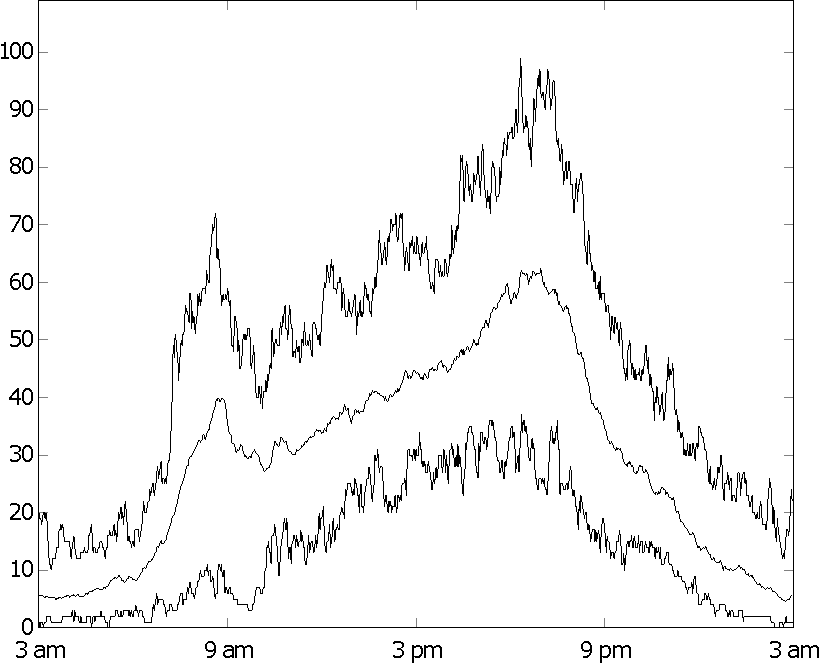
\includegraphics[width=\textwidth]{graphic/Trip_Distribution}
	\caption{Distribution of trips (\cite[p.~62]{Kaiser}, \cite[p.~62]{Knoll})}
	\label{fig:trip_distribution}
\end{figure}

We aim to receive customers with several alternative routes. All routes of the same customer lie in a similar time window. Therefore we first create a set of customers. For each customer we determine a start and end position and a start time. The distribution of the customers' start times is similar to the distribution of the trips in \Cref{fig:trip_distribution}. We do not make the customers to be simple copies of the given trip set over a full instance. Instead we set the start and end positions randomly. We split the full instances into time periods of one hour, starting at each full hour. For each time period we create customers as follows:
\begin{enumerate}
	\item Determine the average number $k$ of trips starting in this time period by the given distribution.
	\item Take a sample of $k$ trips out of $\widehat{\mathcal{T}}$, use their start positions and times for the customers.
	\item Use the end positions of another sample of $k$ trips as end positions for the customers.
	\item Shift all start times by a full hour such that they start in the respective time period.
\end{enumerate}

With this procedure we create the customer set $\mathcal{C}$ with a preliminary start and end position and start time for each customer. Note that in general this preliminary start time does not coincide with $\zstart_c$ which is used in the mathematical models.

\paragraph{Route Creation} \parfill

For each customer we need a set of multimodal routes. Each route roughly starts at the preliminary start time of its customer. It further contains at least one car trip. For each customer there are routes with more than one car trip. In reality, such a route comprises a car trip, a public transport trip and then another car trip. Optionally, there are walking trips in-between. This is the only realistic possibility to gain routes with more than one car trip. Neither two car trips in a row nor a car trip between two public transport trips are a desirable option. The existence of routes with more than one car trip is crucial in order to test the developed solution approaches completely.

The multimodal routes are created with the open source software OpenTripPlanner (cf.~\cite{OTP}). The input for this software is a start and end position and a start time. For each input, it provides several alternative multimodal routes, that comprise car, public transport and walking trips. A great restriction of these route is that they contain only one car trip and this car trip is always at the beginning. In order to receive the required test instances, we have to think of appending a car trip to the existing routes in a realistic way. For this, we do a reverse search from the end point to the start point and identify the station at which the public transport trip starts. Then we search for a multimodal route to this station and append a car trip from this station to the end position. This gives us a multimodal route that starts and ends with a car trip.

For each customer, we are given a start and end position and a start time. We create the routes as follows:
\begin{enumerate}
	\item Request a reverse search from the end position to the start position. Restrict the search to 3 alternative routes. For each alternative, identify the station where the public transport trip starts.
	\item For each station, request a search from the start position to the station. Restrict the search to one alternative. Append a direct car trip from the station to the end position.
	\item Request a search from the start position to the station. Restrict the search to 3 alternatives.
	\item Create a route with a direct car trip from the start to the end position
\end{enumerate}

We use the customer start time as the start time for each search request. From each route, we extract the car trips. They are the only trips that are part of the problem input. With this procedure we create the multimodal route set~$\mathcal{M}$ and the trip set~$\mathcal{T}$ with up to 7 alternative routes and 10 trips for each customer.

\paragraph{Vehicles and Refuel Points} \parfill

Besides trips, a test instance contains vehicles and refuel points. Depending on the requested vehicle number, we take a sample of the previous vehicle set. If this does not suffice, \ie the requested vehicle number is greater than the vehicle set, we additionally create vehicles with the trips' end positions as starting positions of the vehicles. Since we do not have further information about the availability of the vehicles, we choose 2:00~am as the starting time of all vehicles. For the refuel point set, we use a sample of the existing refuel point set with the requested size.

\section{Fuel and Cost}

We need to determine the distances and times between two points for the fuel states and the costs. We compute these values with the open source software OpenSourceRoutingMachine (cf.~\cite{OSRM}). The input are start and end positions and it provides the time and distance between each pair of start and end positions. We request the distances~$d$ and the times~$t$ for
\begin{align*}
	& d_{s,t} && t_{s,t} && \text{for all } s\in\mathcal{V}\cupdot\mathcal{T}\cupdot\mathcal{R}, t\in\mathcal{T}\cupdot\mathcal{R} \\
	& d_t && t_t && \text{for all } t\in\mathcal{T}
\end{align*}

and set the end times ${\zend_t := \zstart_t + t_t}$ for ${t\in\mathcal{T}}$.

\paragraph{Fuel States} \parfill

We assume that the fuel consumption depends linearly on the driven distance of the electrically powered vehicles and the refuel rate depends linearly on the time the vehicle stays at the refuel point. The fuel state of a vehicle is always in the interval $[0,1]$. We introduce the constants $v^{\operatorname{range}}$ which describes the maximal range of a vehicle and $v^{\operatorname{refuel}}$ which describes the maximal refueling time. Therefore the fuel consumption is given by
\begin{align*}
	\fd_{s,t} := \frac{d_{s,t}}{v^{\operatorname{range}}} && \text{for } s\in\mathcal{V}\cupdot\mathcal{R}\cupdot\mathcal{T}, t\in\mathcal{R}\cupdot\mathcal{T} && && \ft_t := \frac{d_t}{v^{\operatorname{range}}} && \text{for } t\in\mathcal{T}
\end{align*}

The refuel rate is fiven by
\begin{align*}
	\ft_r := -\frac{\zstart_t - \zend_s - t_{s,r} - t_{r,t}}{v^{\operatorname{refuel}}} && \text{for all } r\in\Rst
\end{align*}

Since we do not have further information about the fuel states of the vehicles, we set
\begin{align*}
	f^0_v := 1 && \text{for all } v\in\mathcal{V}
\end{align*}

As realistic values we assume that the vehicle range is 135km and the refueling time is 8h. Therefore we set ${v^{\operatorname{range}} =}$~135,000 and ${v^{\operatorname{refuel}} =}$~28,800.

\paragraph{Costs} \parfill

The costs also depend linearly on the driven distance. The constant $c^{\operatorname{meter}}$ describes the cost for each meter a vehicle drives. Thus we set
\begin{align*}
	\cd_{s,t} := c^{\operatorname{meter}}\cdot d_{s,t} && \text{for } s\in\mathcal{V}\cupdot\mathcal{R}\cupdot\mathcal{T}, t\in\mathcal{R}\cupdot\mathcal{T} && && \ct_t := c^{\operatorname{meter}}\cdot d_t && \text{for } t\in\mathcal{T}
\end{align*}

We set the constants ${c^{\operatorname{meter}} =}$~1 and ${\cv =}$~50,000.

The only cost left is the route cost. As mentioned in \Cref{sec:problem_description}, we use the route cost in order to model a realistic customer behavior. It contains the cost for public transport and the user inconvenience that arises if the customer chooses this route. We approximate the public transport cost in comparison to cost for car sharing. The constant $c^{\operatorname{public}}$ describes the cost for using public transport. The main user inconveniences are the total travel time and the walking time. The constants $c^{\operatorname{time}}$ and $c^{\operatorname{walk}}$ describe the respective penalty costs.

Based on the charges of Car2Go (cf.~\cite{Car2Go}), we assume that a customer pays in average 0.50 euros per kilometer driving with a car. Due to the public transport provider in Stuttgart (cf.~\cite{VVS}), we assume that a customer pays in average 6 euros per hour using public transport. In order to compare the user inconveniences, we additionally charge 10 euros per hour for the total travel time and 10 euros per hour walking.

\paragraph{Example} \parfill

In order to illustrate the procedure that we have developed before, we show an example of a multimodal route.

\begin{example}

Consider that the route as described in \Cref{tab:exemplary_route} has been developed in \Cref{sec:trip_creation}. 

\begin{table}[htb]
	\centering
	\begin{tabular}{cccccc}
		Time & Mode & $d_t$ & $\ct$ & $\croute$ & Cost \\
		\hline
		8:00 - 8:12 & Car & 6km & 6000 & & 3.00 euros \\
		8:12 - 8:15 & Walk & & & 1000 & 0.50 euros \\
		8:15 - 8:25	& Subway & & & 2000 & 1.00 euros \\
		8:25 - 8:28 & Wait & & & & \\
		8:28 - 8:33 & Bus & & & 1000 & 0.50 euros \\
		8:33 - 8:39 & Walk & & & 2000 & 1.00 euros \\
		8:39 - 8:45 & Car & 3km & 3000 & & 1.50 euros
	\end{tabular}
	\caption{Exemplary route}
	\label{tab:exemplary_route}
\end{table}

Only the car trips of this route are part of the input. Thus we have $t_1,t_2\in\mathcal{T}$. We call the route ${m=\left(t_1,t_2\right)}$ and the associated customer $c\in\mathcal{C}$. The trips have the values:
\begin{align*}
	\zstart_{t_1} = \text{8:00pm} && \zend_{t_1} = \text{8:12pm} && \ct_{t_1} = 6000 && \ft_{t_1} = 0.044 \\
	\zstart_{t_2} = \text{8:39pm} && \zend_{t_2} = \text{8:45pm} && \ct_{t_2} = 3000 && \ft_{t_2} = 0.022
\end{align*}

The route cost comprises a penalty of 15,000 for the total travel time and in summary we have ${\croute_m =}$~21,000.

\end{example}

\section{Instance Sizes}




%----------------------------------------------------------------------------------------------------------------------------------------

%\section{Route Creation}
%
%We are not given the set of routes $\mathcal{M}$ in advance. For each customer $c\in\mathcal{C}$, we have start and end location $\pstart_c, \pend_c$ and a start and end time $\zstarto_c, \zendo_c$. All the trips of the customer lie in this interval, i.e.
%
%\begin{align*}
	%\zstarto_c \leq \zstart_m && \zend_m \leq \zendo_c && \text{for all } m\in C^{-1}(c).
%\end{align*}
%
%\paragraph{Basic Restrictions} \parfill
%
%To simplify the creation of the routes, we make some assumptions. For every route $m\in\mathcal{M}$ holds:
%
%\begin{itemize}
	%\item{There are not two car trips in a row.}
	%\item{There is no car trip between two public transport trips.}
	%\item{The number of public transport trips is restricted. Usually, one can reach every station with at most two changes.}
	%\item{We define a walking distance $d^{\operatorname{walk}}$. If the distance between the start position and the first station or between the last station and the end position, there is no car trip necessary.}
%\end{itemize}
%
%We assume that we have some oracle that provides the set of feasible public transport routes for customer $c\in\mathcal{C}$:
%
%\begin{align*}
	%M_c & = && \left\{\left(s_1,z_1,s_2,z_2\right)|s_1,s_2\in\mathcal{S}, \zstarto_c\leq t_1 < t_2 \leq \zendo_c, \text{ there is a public} \right. \\
	%&&& \left.\vphantom{\zstarto}\text{transport route from $s_1$ to $s_2$ with start time $z_1$ and end time $z_2$}\right\}
%\end{align*}
%
%The fact, whether the customer changes during his usage of public transport, has no effect on the model. Thus, we can consider each element in $M_c$ as a public transport trip.
%
%\paragraph{Route Creation} \parfill
%
%We create the set of multimodal routes $\mathcal{M}$. For this, we set a car trip before and after each public transport trip in order to bring the customer from his start to his destination, except when it is possible to walk the distance. We also have to consider the given time restrictions. Further, we create the pure car trips. How the set $\mathcal{M}$ is created in detail, is described in \Cref{alg:route_creation}.
%
%Until now, we do not consider any changing times between a car trip and a public transport trip.
%
%Further, we assume that the given customer start and and times are feasible, i.e. $\zstarto_c+t_{\pstart_c,\pend_c}\leq\zendo_c$ for all $c\in\mathcal{C}$.
%
%\begin{algorithm}
	%\SetAlgoLined
	%\KwIn{customer set $\mathcal{C}$; $\pstart_c, \pend_c, \zstarto_c, \zendo_c, M_c$ for all $c\in\mathcal{C}$}
	%\KwOut{set of routes $\mathcal{M}$, set of trips $\Tcar,\Tpub$}
	%$\Tcar\gets\emptyset$\;
	%$\Tpub\gets\emptyset$\;
	%$\mathcal{M}\gets\emptyset$\;
	%\ForEach{$c\in\mathcal{C}$}{
		%\ForEach{$\left(s_1,z_1,s_2,z_2\right)\in M_c$}{
			%create public transport trip $t$\;
			%$\pstart_t\gets s_1,\pend_t\gets s_2,\zstart_t\gets z_1,\zend_t\gets z_2$\;
			%create car trips $t_1,t_2$\;
			%$\pstart_{t_1}\gets\pstart_c,\pend_{t_1}\gets s_1,\zstart_{t_1}\gets z_1 - t_{\pstart_c,s_1},\zend_{t_1}\gets z_1$\;
			%$\pstart_{t_2}\gets s_2,\pend_{t_2}\gets\pend_c,\zstart_{t_2}\gets z_2,\zend_{t_2}\gets z_2 + t_{s_2,\pend_c}$\;
			%\If{$\zstarto_c\leq\zstart_{t_1} \land \zend_{t_2}\leq \zendo_c$}{
				%create multimodal route $m$\;
				%$\Tpub\gets\Tpub\cup \{t$\}\;
				%\lIf{$d_{\pstart_c,s_1}\geq d^{\operatorname{walk}}$}{$m\gets\left(t_1,t\right)$; $\Tcar\gets\Tcar\cup\left\{t_1\right\}$}
				%\lElse{$m\gets\left(t\right)$}
				%\lIf{$d_{s_2,\pend_c}\geq d^{\operatorname{walk}}$}{append $t_2$ to $m$; $\Tcar\gets\Tcar\cup\left\{t_2\right\}$}
				%$C(m)\gets c$\;
				%$\mathcal{M}\gets\mathcal{M}\cup\left\{m\right\}$\;
				%}
		%}
		%create car trips $t_1,t_2$\;
		%$\pstart_{t_1}\gets\pstart_c,\pend_{t_1}\gets\pend_c,\zstart_{t_1}\gets\zstarto_c,\zend_{t_1}\gets\zstarto_c + t_{\pstart_c,\pend_c}$\;
		%$\pstart_{t_2}\gets\pstart_c,\pend_{t_2}\gets\pend_c,\zstart_{t_2}\gets\zendo_c - t_{\pstart_c,\pend_c},\zend_{t_2}\gets\zendo_c$\;
		%create multimodal routes $m_1,m_2$\;
		%$m_1\gets\left(t_1\right), m_2\gets\left(t_2\right)$\;
		%$\Tcar\gets\Tcar\cup\left\{t_1,t_2\right\}, \mathcal{M}\gets\mathcal{M}\cup\left\{m_1,m_2\right\}$\;
	%}
	%\Return{$\mathcal{M},\Tcar,\Tpub$}
	%\caption{Creation of the routes \label{alg:route_creation}}
%\end{algorithm}
%
%\paragraph{Further Restrictions} \parfill
%
%If the routes are created as described in \Cref{alg:route_creation}, there are routes using every available station as long as it is feasible. Most of these routes are obviously bad for the customer since they cause a big detour. What is more, a large number of routes enlarge the problem size and leads to  a bad performance for solving it. Therefore, we try to restrict the set of alternatives to a reasonable size.
%
%\begin{example}
%
%Let $\mathcal{S}=\left\{s_1,\dots,s_n\right\}$ with a single public transport ride serving all stations. Let $\mathcal{C}=\left\{c_1,c_2\right\}$ with $\pend_{c_1}=s_n$ and $\pstart_{c_2}=s_k$ for a certain $k\in[n-1]$. The alternative routes are
%
%\begin{align*}
	%\mathcal{M} = \underbrace{\left\{\left(\left(\pstart_{c_1},s_i\right),\left(s_i,s_n\right)\right)|i\in[n-1]\right\}}_{\text{for }c_1}\cup\underbrace{\left\{\left(s_k,\pend_{c_2}\right)\right\}}_{\text{for }c_2}
%\end{align*}
%
%with $\left(\pstart_{c_1},s_k\right)\prec\left(s_k,\pend_{c_2}\right)$ and $\left(\pstart_{c_1},s_i\right)\not\prec\left(s_k,\pend_{c_2}\right)$ for all $i\in[n]\backslash\{k\}$. 
%
%We get the only solution, where only one car is needed, when $c_1$ drives to $s_k$, wherever the station $s_k$ is. Every route of $c_1$ can be the optimal route, considering the other customers. Therefore, an exact reduction of $\mathcal{M}$ is not possible without the the risk of cutting off the optimal solution.
	%
%\end{example}
%
%It is not practicable to consider all possible multimodal routes due to computation reasons. But it is also not possible to reduce the number of routes without risking to lose the optimal solution. Hence, we try to make reasonable restrictions which keep the problem size small.
%
%\paragraph{Pareto Optimality} \parfill
%
%The idea is to choose only Pareto optimal multimodal routes (cf. Kaiser/Knoll, cap. 3.2.2) in order to determine good routes.
%
%\begin{definition}[Pareto optimality]
%
%Let $V\subset\mathbb{R}^n$.
%
%\begin{enumerate}
	%\item{The partial order $\leq$ on $\mathbb{R}^n$ is given by
		%\begin{align*}
			%v\leq w && :\Leftrightarrow && v_i\leq w_i && \forall i\in[n] && \text{for all }v,w\in\mathbb{R}^n
		%\end{align*}}
	%\item{An element $w\in V$ is Pareto optimal in $V$ if it is minimal with respect to $\leq$ in $V$, i.e.
		%\begin{align*}
			%v\leq w && \Rightarrow && v=w && \text{for all } v\in V
		%\end{align*}}
	%\item{The Pareto frontier of $V$ with respect to $\leq$ is the set of Pareto optimal elements in $V$, i.e.
		%\begin{align*}
			%\operatorname{min}_{\leq} V := \left\{w\in V|\forall v\in V: v\leq w \Rightarrow v=w\right\}
		%\end{align*}}
%\end{enumerate}
%
%\end{definition}
%
%Let $m\in\mathcal{M}$ be a multimodal route. We define
%
%\begin{align*}
	%\varphi:\mathcal{M}\to\mathbb{R}^5 && m\mapsto\left(
	%\begin{array}{c}
		%\croute + \sum_{t\in m\cap\Tcar}\ct_t \\
		%\croute \\
		%|\Tcar\cap\{t\in m\}|\\
		%\sum_{t\in m\cap\Tcar} \zend_t - \zstart_t \\
		%\sum_{t\in m\cap\Tcar} \ft_t
	%\end{array} \right)
%\end{align*}
%
%The function $\varphi$ grades a route to their costs, their route costs, the number of cars needed, the time of a car needed and the fuel consumption.
%
%From now on, we will use the Pareto frontier of $\varphi\left(\mathcal{M}\right)$ as a restricted route set:
%
%\begin{align}
	%\hat{\mathcal{M}} := min_{\leq} \varphi\left(\mathcal{M}\right)
%\end{align}

\backmatter

\appendix

\section{Previous Formulations}

\subsection{MILP}

\begin{align}
	\min & \sum_{s\in\mathcal{V}} \sum_{t\in\Nout(s)\backslash\{d^{\operatorname{e}}\}} x_{s,t}c^{\operatorname{v}} \nonumber \\
	& \omit\rlap{$\displaystyle{ + \sum_{t\in\mathcal{T}} \sum_{s\in\Nin(t)} \left[x_{s,t}\left(c_{s,t}^{\operatorname{d}}+c_{t}^{\operatorname{t}}\right) + \sum_{r\in\Rst} z_{s,r,t}\left(c_{s,r}^{\operatorname{d}}+c_{r,t}^{\operatorname{d}}-c_{s,t}^{\operatorname{d}}\right)\right]}$} \tag{MILP} \label{eq:MILP} \\
	\text{s.t.} & \sum_{t\in\Nin(s)} x_{t,s} = \sum_{t\in\Nout(s)} x_{s,t} & & \text{for all } s\in V\backslash\left\{d^{\operatorname{s}},d^{\operatorname{e}}\right\} \tag{3.15} \\
	& \sum_{s\in\Nin(t)} x_{s,t} = 1 & & \text{for all } t\in\mathcal{V} \tag{3.16} \\
	& \sum_{t\in C^{-1}(c)} \sum_{s\in\Nin(t)} x_{s,t} = 1 & & \text{for all } c\in\mathcal{C} \tag{3.17} \label{eq:costumer} \\
	& \sum_{r\in\Rst} z_{s,r,t} \leq x_{s,t} & & \text{for all } t\in\mathcal{T}, s\in\Nin(t) \tag{3.18} \\
	& e_s \leq f_s^0 & & \text{for all } s\in\mathcal{V} \tag{3.19} \\
	& 0 \leq e_s - \sum_{r\in\Rst} z_{s,r,t}\fd_{s,r} & & \text{for all } t\in\mathcal{T}, s\in\Nin(t) \tag{3.12} \\
	& e_t \leq 1 - \ft_t - \sum_{r\in\Rst} z_{s,r,t}\fd_{r,t} & & \text{for all } t\in\mathcal{T}, s\in\Nin(t) \tag{3.13} \\
	& \omit\rlap{$\displaystyle{e_t \leq e_s - x_{s,t}\left(f_{s,t}^{\operatorname{d}}+f_t^{\operatorname{t}}\right) - \sum_{r\in\Rst} z_{s,r,t}\left(\fd_{s,r}+\ft_r+\fd_{r,t}-\fd_{s,t}\right) + \left(1-x_{s,t}\right)}$} \nonumber \\
	& & & \text{for all } t\in\mathcal{T}, s\in\Nin(t) \tag{3.14} \\
	& x_{s,t}\in\{0,1\} & & \text{for all } (s,t)\in A \tag{3.20} \\
	& z_{s,r,t}\in\{0,1\} & & \text{for all } t\in\mathcal{T},s\in\Nin(t),r\in\Rst \tag{3.21} \\
	& e_s\in[0,1] & & \text{for all } s\in V\backslash\left\{d^{\operatorname{s}},d^{\operatorname{e}}\right\} \tag{3.22}
\end{align}

\subsection{AMILP}

\begin{align}
	\min & \sum_{s\in\mathcal{V}} \sum_{t\in\Nout(s)\backslash\{d^{\operatorname{e}}\}} x_{s,t}c^{\operatorname{v}} \nonumber \\
	& \omit\rlap{$\displaystyle{ + \sum_{t\in\mathcal{T}} \sum_{s\in\Nin(t)} \left[x_{s,t}\left(c_{s,t}^{\operatorname{d}}+c_{t}^{\operatorname{t}}\right) + \sum_{r\in\Rst} z_{s,r,t}\left(c_{s,r}^{\operatorname{d}}+c_{r,t}^{\operatorname{d}}-c_{s,t}^{\operatorname{d}}\right)\right]}$} \tag{AMILP} \label{eq:AMILP} \\
	\text{s.t.} & \sum_{t\in\Nin(s)} x_{t,s} = \sum_{t\in\Nout(s)} x_{s,t} & & \text{for all } s\in V\backslash\left\{d^{\operatorname{s}},d^{\operatorname{e}}\right\} \tag{3.15} \\
	& \sum_{s\in\Nin(t)} x_{s,t} = 1 & & \text{for all } t\in\mathcal{T}\cup\mathcal{V} \tag{6.2} \\
	& \sum_{r\in\Rst} z_{s,r,t} \leq x_{s,t} & & \text{for all } t\in\mathcal{T}, s\in\Nin(t) \tag{3.18} \\
	& e_s \leq f_s^0 & & \text{for all } s\in\mathcal{V} \tag{3.19} \\
	& 0 \leq e_s - \sum_{r\in\Rst} z_{s,r,t}\fd_{s,r} & & \text{for all } t\in\mathcal{T}, s\in\Nin(t) \tag{3.12} \\
	& e_t \leq 1 - \ft_t - \sum_{r\in\Rst} z_{s,r,t}\fd_{r,t} & & \text{for all } t\in\mathcal{T}, s\in\Nin(t) \tag{3.13} \\
	& \omit\rlap{$\displaystyle{e_t \leq e_s - x_{s,t}\left(f_{s,t}^{\operatorname{d}}+f_t^{\operatorname{t}}\right) - \sum_{r\in\Rst} z_{s,r,t}\left(\fd_{s,r}+\ft_r+\fd_{r,t}-\fd_{s,t}\right) + \left(1-x_{s,t}\right)}$} \nonumber \\
	& & & \text{for all } t\in\mathcal{T}, s\in\Nin(t) \tag{3.14} \\
	& x_{s,t}\in\{0,1\} & & \text{for all } (s,t)\in A \tag{3.20}\\
	& z_{s,r,t}\in\{0,1\} & & \text{for all } t\in\mathcal{T},s\in\Nin(t),r\in\Rst \tag{3.21} \\
	& e_s\in[0,1] & & \text{for all } s\in V\backslash\left\{d^{\operatorname{s}},d^{\operatorname{e}}\right\} \tag{3.22}
\end{align}



\bibliography{Literatur}
\bibliographystyle{alpha}

\listoffixmes

\end{document}